	\documentclass[12pt,a4paper]{report}
\usepackage{amsmath}
\usepackage{amsfonts}
\usepackage{amssymb}
\usepackage[english]{babel} %type ngerman if you are using a PC of the university
\usepackage{babelbib}
\usepackage[T1]{fontenc}
\usepackage[sc]{mathpazo}
\usepackage[utf8]{inputenc}
\usepackage{graphicx}
\usepackage[width=150mm,top=25mm,bottom=25mm]{geometry}
%\usepackage{units}
\usepackage{fancyhdr}
\pagestyle{fancy}

\renewcommand{\chaptermark}[1]{\markboth{#1}{}}

%Chapter title on even header and section title in odd header
\fancyhf{} % clear the headers
\fancyhead[R]{%
   % We want italics
   \itshape
   % The chapter number only if it's greater than 0
   \ifnum\value{chapter}>0 \chaptername\ \thechapter. \fi
   % The chapter title
   \leftmark}
\fancyfoot[C]{\thepage}

\fancypagestyle{plain}{
  \renewcommand{\headrulewidth}{0pt}
  \fancyhf{}
  \fancyfoot[C]{\thepage}
}

\setlength{\headheight}{14.5pt}
\makeatletter
\setlength{\@fptop}{0pt}
\makeatother
%\usepackage{kantlipsum} % for the mock text
\usepackage{enumerate} % enumerados
\usepackage{float} % here for H placement parameter
\usepackage[section]{placeins}
\usepackage{colortbl}
\usepackage{xcolor}
\definecolor{mygray}{gray}{0.8}
\usepackage{xfrac}
\usepackage{booktabs} 
\usepackage{colortbl} 
\usepackage{color}   %May be necessary if you want to color links
\usepackage{hyperref}
\usepackage{setspace}
\usepackage{caption}
\usepackage{subcaption}
\usepackage{titlesec}
\usepackage{tikz}
\usepackage{amsmath}
\usetikzlibrary{calc,positioning,shadows.blur,decorations.pathreplacing}
\usepackage{etoolbox}
\usepackage{anyfontsize}
\usepackage[toc,page]{appendix}
%\titleformat{\chapter}{\normalfont\bfseries}{\thechapter}{1em}{\Huge}
\titleformat{\chapter}{\normalfont\bfseries}{\huge\thechapter}{1em}{\Huge}
\usepackage{nicefrac}
\onehalfspacing
\hypersetup{
    colorlinks=false, %set true if you want colored links
    linktoc=all,     %set to all if you want both sections and subsections linked
    linkcolor=blue,  %choose some color if you want links to stand out
	}
\author{Youssef El Mard Bouziani}
\title{Transversalimpulsverteilung geladener Teilchen in Proton-Proton-Kollisionen bei  $\sqrt{s} = 5.02$ TeV in ALICE}
\parindent 0ex



\begin{document}
%NEW COMMANDS
%https://texample.net/media/tikz/examples/PDF/periodic-table-of-chemical-elements.pdf
\newcommand{\Quark}[5]
{
  \begin{minipage}{0.cm}
    %\centering
      %{\scriptsize \text{#1}  \hfill  \footnotesize #2}%
      {\hfill \footnotesize \text{ #3} }
        % {\centering \footnotesize \textbf{#5}\\}
  \end{minipage}
 {\raisebox{40pt}{\makebox[1em][l]{\footnotesize \textbf{#1}}}%
 \hspace{2.3cm} \raisebox{40pt}{\makebox[3em][l]{\footnotesize \textbf{#2} }} \hspace{-3.1cm} 
 \parbox[t][1em]{3em}{\centering{\fontsize{40}{40}\selectfont  #4}	}\hspace*{1em}   %Amb \parbox[t][1em]{2em} es la carga electrica surt del requadre     
    \parbox[c][6em]{0em}{\vspace{1.4cm}\hspace{-2.7cm}\centering \footnotesize \textbf{#5}}   
}
}
  \tikzstyle{QuarkFill} = [fill=blue!15]
  \tikzstyle{LeptonFill} = [fill=red!15]
  \tikzstyle{BosonFill} = [fill=green!15]
  \tikzstyle{quark} = [draw=blue, very thick, rounded corners=2mm, QuarkFill,  minimum height={2.6cm+2pt}, minimum width=2.cm, node distance=2.cm ]
    \tikzstyle{lepton} = [draw=red, very thick, rounded corners=2mm, LeptonFill,  minimum height={2.6cm+2pt}, minimum width=1.5cm, node distance=2.cm ]
    \tikzstyle{boson} = [draw=green, very thick, rounded corners=2mm, BosonFill,  minimum height={2.6cm+2pt}, minimum width=1.5cm, node distance=2.cm ]
   
\newcommand{\pt}{$p_\text{T}$ }
\newcommand{\raa}{$R_\text{AA}$ }
\newcommand{\rled}{$R_\text{PbPb}$ }
\definecolor{headerBlue}{RGB}{104, 104, 255} %blue RICHTIG headerBlue
\definecolor{headerRed}{RGB}{126, 0, 33} %red
\definecolor{bodyBlue}{RGB}{228,232,244} %light blue

\begin{titlepage}
\begin{center}

\vspace*{4cm}  

\huge{\textbf{Nuclear Modification of charged-particles production at $\sqrt{s_\text{NN}} = 5.02$ TeV in ALICE}}\\[2cm]
\vfill
\Large{\textbf{Master thesis}}\\
Institut für Kernphysik Frankfurt\\
\vfill
%presented by\\[1cm]
by \Large{\textbf{Youssef El Mard Bouziani}}\\[1cm]
\vfill
Fachbereich Physik\\
der Goethe-Universität\\
Frankfurt am Main\\
\vspace*{1cm}
April 2021
\end{center}
\end{titlepage}


\vspace*{22cm}
\large{Erstgutachter: Prof. Dr. Henner Büsching}\\
\large{Zweitgutachter: Prof. Dr. Harald Appelshäuser}
\normalsize
\pagenumbering{roman}
\newpage
\tableofcontents
\newpage

\pagenumbering{arabic}
\setcounter{chapter}{-1}
\pagenumbering{arabic} 
\chapter{Abstract}
The insights gained in the field of particle physics during the 20th century set in motion a revolution in the view of the world that had prevailed up to that point. Various postulates about the structure of matter, which could later be proven experimentally, taught us that matter consists of a few elementary building blocks. The standard model of particle physics was developed to summarise all the findings about elementary particles and their interactions.\\
The quark gluon plasma (QGP) has occupied a prominent position in high-energy physics as the subject of current research for decades. This is reflected, among other things, in the fact that one of the four largest experiments at the currently most powerful particle accelerator in the world, the LHC, the ALICE experiment, is almost exclusively concerned with the study of this special state of matter. The presended thesis deals with one aspect of the study of the properties of the QGP, the analysis of the production of unidentified charged particles in the ALICE experiment.\\
The master's thesis investigates lead-lead collisions at a centre-of-mass energy per nucleon pair of $\sqrt{s_\text{NN}}$ = 5.02 TeV, which were recorded with the ALICE detector in 2017. According to the current state of knowledge, the experimental production of a QGP is only possible in heavy-ion collisions; however, other collision systems are also investigated as reference measurements, for example proton-proton collisions. A comparison of the results of both analyses then allows conclusions to be drawn about the differences in the respective production mechanisms and thus to be able to make statements about the properties of a QGP. In the ALICE experiment, electrically charged particles can be detected with very high accuracy using the experiment's track detectors. My work deals with the measurement of these particles produced in the collisions as a function of their momentum fraction orthogonal to the beam axis, the so-called transverse momentum pT. If a QGP is formed in the lead-lead collisions, the production of these particles should change significantly. From the comparison of the pT distribution of these particles with theoretical models, information about the properties of the QGP can then be obtained.\\
In my work, a variety of selection criteria are used that aim to ensure the best possible data quality for further analysis. More precisely, these selection criteria refer to properties of the tracks left by the particles in the detector. Thus, for example, only particles that originate directly from a collision, i.e. primary particles, can be selected. In contrast, particles that result from interaction with the detector material or from certain decay processes, the so-called secondary particles, are excluded from the analysis.\\
After applying these selection criteria, a transverse momentum distribution results, which is, however, still influenced by numerous detector effects: For example, a small fraction of secondary particles remains even after the track selection. In addition, not all particles are seen by the detectors; this must be corrected in the work by the so-called detection efficiency, the probability with which particles are recorded. In the thesis, the transverse momentum distribution is corrected for this using so-called Monte Carlo simulations. The investigation of these detector effects and the development of the necessary corrections are an important part of the analysis. In my work, I can draw on methods that have been developed for this purpose for years by the members of the ALICE working group. With the help of the corrections, the final transverse momentum distributions in proton-proton and in lead-lead collisions can then be extracted. In the work, the transverse momentum distributions for lead-lead collisions are divided into nine centrality intervals. As described in the PhD project, it is now suspected that the probability for the formation of a QGP is higher in central collisions than in peripheral collisions. 
The comparison between the particle production in proton-proton collisions with that in lead-lead collisions is done in the thesis by calculating the nuclear modification factor. This fundamental quantity is determined by forming the ratio of the measured transverse momentum distribution in a centrality range and the correspondingly scaled reference measurement in proton-proton collisions. The number of binary nucleon-nucleon collisions in lead-lead collisions is used as the scaling factor. A nuclear modification factor of one would then mean that a heavy ion collision behaves like a superposition of nucleon-nucleon collisions. However, nuclear modification factors smaller than one are observed, indicating the existence of a medium in lead-lead collisions that suppresses particle production and could correspond to the expected QGP. Furthermore, it can be shown that the nuclear modification factor increases for peripheral collisions. This confirms the above idea that the energy density increases with centrality.\\
Finally, the paper discusses the results by comparing them with published results from an analogous analysis of data recorded in 2015, which have lower statistics than the new data. The dataset studied in my work thus allows for finer granularity and increased coverage of the transverse momentum distributions as well as the nuclear modification factors. This allows significant progress to be made in the more detailed study of the properties of the QGP.
\chapter{Introduction}
\section{The Structure of Matter}
\label{sec:DasSMT}
Throughout the twentieth century, successive crucial advances in the field of particle physics led to a revolution of the world-view on the structure of matter and the fundamental forces that govern the universe. Following these developments, it became necessary to consolidate the acquired knowledge into a single theory: the Standard Model, which marked by the end of the 1970s the foundation of modern particle physics. This systematization provided from a theoretical point of view subsequently confirmed experimentally a comprehensive description of the nature of elementary particles and the fundamental interactions they mediate: the electromagnetic, the weak and the strong interaction. \\
All matter in the universe is composed of indivisible particles that lack spatial extent and substructure, the so-called elementary particles. The first particles to be proposed as elementary were the atoms. This picture changed in the early 20th century after it was proved that atoms are made up of a nucleus constituted by protons and neutrons, around which electrons orbit. In the subsequent decades, an extensive number of other subatomic particles were discovered, raising the question among physicists of whether all of them were in fact structureless. The Standard Model sorted out this confusion, historically known as particle zoo, describing the existence of a low number of elementary particles subdivided into two types named quarks and leptons that build all known particles, including protons and neutrons. In addition, the Standard Model clarified that the interactions between quarks and leptons occur by means of an exchange of force-carrier particles, also considered elementary. \\
In order to classify the elementary particles, it is required to consider the immutable and distinguishable physical properties each of them possess. In this regard, the most fundamental distinction between the building blocks of matter and the force-carrier particles lies in the intrinsic angular momentum, known generally as spin, all particles carry, whether or not they are elementary. Particles of half-integer spin in units of the Planck's constant $\hbar$ are named fermions and present an antisymmetric wave function, whereas those of integer spin are known as bosons and their wave function describes a symmetric behavior. In this context, quarks and leptons are considered elementary fermions since their spin is equal to $\nicefrac{\pm 1}{2}$, while the force-carriers, which have a spin $1$, are referred to as gauge bosons.\\
The Standard Model states the existence of six quarks and six leptons, summarized in Figure \ref{SM}. Both groups of elementary fermions are arranged according to the mass in three doublets named generations. Each pair of quarks or leptons have a mass one or two orders of magnitude lower than the pair of the next generation. Furthermore, the electrical charge is another feature used to sort elementary fermions. The triplets composed of elementary fermions from different generations have the same electrical charge, namely $\nicefrac{+2}{3}$ and $\nicefrac{-1}{3}$ for the case of the quarks and $0$ and $-1$ for the one of the leptons. The Standard Model predicts also the occurrence in Nature of antiquarks and antileptons, elementary fermions with identical mass as their counterparts but opposite electrical charge and spin.  \\
The six species or flavours of quarks known at the present day are up $u$, down $d$, charm $c$, strange $s$), top $t$ and bottom $b$. At this point, it should be emphasized that quarks could not yet be observed existing on their own, but only building bound states named hadrons. These composite particles, detected for the first time during the era of the particle zoo, come in two types: hadrons built from three different quarks are called baryons, while those constituted of a quark-antiquark pair mesons. For instance, the quark composition of protons and neutrons, respectively \textit{uud} and \textit{udd}, 
allows to identify them as baryons. All known hadrons, excluding the proton, decay after a given period of time. It should be also noted that since the spin is an additive property, baryons are considered fermionic particles and mesons, by contrast, bosonic particles. \\
The quark composition of a hadron determines intrinsic facets of the particle, which are associated with additive quantities named quark quantum numbers: the well-known electrical charge, a parametrization of the number of quarks called baryon number \textit{B} and other parametrization of the second- and third-generation flavours. However, the valence quarks, i.e. the quarks that determine the identity of a hadron, aren't the only components. In fact, a hadron should be understood as a more complex and dynamic structure that contains, aside from the valence quarks, an amalgam of quark-antiquark pairs named sea quarks in a constant process of creation and annihilation as well as a large number of gluons, the force-carrier of the strong interaction, which will be discussed later. This picture is consistent with the fact that the sum of the masses of the valence quarks of a given hadron doesn't coincide with the observed mass of the hadron, being this significantly larger.  \\
\begin{figure}
\begin{center}
\begin{tikzpicture}[font=\sffamily, x=1.5cm, y=2cm, scale = 0.35, every node/.style={scale=0.6}]
\centering 
\node[name=u, quark] {\Quark{3 MeV}{$\nicefrac{1}{2}$}{$\nicefrac{+2}{3}$}{$\boldsymbol u$}{up}};
 \node [name=c, right=0.1cm of u, quark] {\Quark{1.24 MeV}{$\nicefrac{1}{2}$}{$\nicefrac{+2}{3}$}{$\boldsymbol c$}{charm}};
  \node [name=t, right=0.1cm of c, quark] {\Quark{172.5 GeV}{$\nicefrac{1}{2}$}{$\nicefrac{+2}{3}$}{$\boldsymbol t$}{top}};
  \node [name=d, below=0.1cm of u, quark] {\Quark{6\text{ MeV}}{$\nicefrac{1}{2}$}{$\nicefrac{-1}{3}$}{$\boldsymbol d$}{down}};
  \node [name=s, below=0.1cm of c, quark] {\Quark{95\text{ MeV}}{$\nicefrac{1}{2}$}{$\nicefrac{-1}{3}$}{$\boldsymbol s$}{strange}};
   \node [name=b, below=0.1cm of t, quark] {\Quark{4.2\text{ GeV}}{$\nicefrac{1}{2}$}{$\nicefrac{-1}{3}$}{$\boldsymbol b$}{bottom}};
   
  \node [name=elneu,  below=0.2cm of d, lepton] {\Quark{<\text{2.2}\text{ eV}}{$\nicefrac{1}{2}$}{$0$}{$\boldsymbol  \nu_e$}{electron neutrino}};
  \node [name=elmuon, right=0.1cm of elneu, lepton] {\Quark{<\text{0.17}\text{ MeV}}{$\nicefrac{1}{2}$}{$0$}{$\boldsymbol  \nu_\mu$}{muon neutrino}};
    \node [name=eltau, right=0.1cm of elmuon, lepton] {\Quark{<\text{15.5}\text{ eV}}{$\nicefrac{1}{2}$}{$0$}{$\boldsymbol  \nu_\tau$}{tau neutrino}};
    
      \node [name=ele,  below=0.1cm of elneu, lepton] {\Quark{0.511\text{ MeV}}{$\nicefrac{1}{2}$}{$-1$}{$\boldsymbol e$}{electron}};
  \node [name=muon, right=0.1cm of ele, lepton] {\Quark{105.7\text{ MeV}}{$\nicefrac{1}{2}$}{$-1$}{$\boldsymbol \mu$}{muon}};
    \node [name=tau, right=0.1cm of muon, lepton] {\Quark{1.777\text{ GeV}}{$\nicefrac{1}{2}$}{$-1$}{$\boldsymbol\tau$}{tau}};
   
 \node [name=gluon,  right=0.2cm of t, boson] {\Quark{$0$}{$1$}{$0$}{$\boldsymbol  g$}{gluon}};
 \node [name=photon,  right=0.2cm of b, boson] {\Quark{$0$}{$1$}{$0$}{$\boldsymbol  \gamma$}{photon}};
 \node [name=gluon,  right=0.2cm of eltau, boson] {\Quark{91.19 GeV}{$1$}{$0$}{$\boldsymbol  Z$}{\textit{Z} boson}};
 \node [name=gluon,  right=0.2cm of tau, boson] {\Quark{80.39 GeV}{$1$}{$\pm$1}{$\boldsymbol  W$}{\textit{W} boson}};
\end{tikzpicture}
 \caption{Elementary particles of the Standard Model. Quarks, leptons and }
 \label{SM}
\end{center}
\end{figure}
\hspace{-0.53cm} As already mentioned, six flavours of leptons are known at this time: three electrically charged leptons, the electron $e$, the muon $\mu$ and the tau $\tau$, and the corresponding electrically neutral leptons that complete each generation, the electron neutrino $\upsilon_{e}$, the muon neutrino $\upsilon_{\mu}$ and the tau neutrino $\upsilon_{\tau}$. In contrast to quarks, leptons don't arrange themselves to form composite particles, with the big exception of the electron shell of an atom, and can exist on their own. \\
According to our actual understanding, all observed phenomenon at subatomic level, such as the formation of composite particles or the particle decays, manifest themselves by means of the existence of three fundamental interactions: the electromagnetic, the weak and the strong interaction. In modern particle physics, each of these interactions is explained as an exchange of quanta of elementary bosons between the elementary particles that exert the force. In order to experience a given fundamental force, an elementary particle must carry the corresponding charge. Particles are charged in different magnitudes, which determines the intensity with they create or undergo the force. \\
The force-carrier particle of the electromagnetic interaction is named photon $\gamma$, a massless boson that mediates the attraction and repulsion forces between all electrically charged particles. In the case of the weak interaction, which all elementary fermions can experience, there are three massive mediators: one electrically neutral, namely the $Z$ boson, and two electrically charged, the $W^{\pm}$ bosons. Finally, the strong interaction is mediated by the already introduced gluon $g$. The charge of the strong interaction is called color, but it should not be mistaken for the concept generally known and described by the optical physics. Quarks are the only elementary fermions that have color charge and therefore gluons can couple to them. In addition to quarks, gluons carry also color what allows them to couple to themselves, a particularity only present in the strong interaction. The basic processes of the strong interaction are described by a theory named quantum chromodynamics (QCD). Since some of these processes represent a key knowledge for the understanding of this thesis, this theory will be treated in the coming section more exhaustive.

\section{Quantum Chromodynamics}
%https://webhome.phy.duke.edu/~kolena/modern/color.html
%Und die drei Bücher
Historically, the concept of colors were introduced in order to remedy an apparent violation of the Pauli's exclusion principle, which states the antisymmetric nature of hadrons. During the early development of quark model, the wave function of hadrons appeared to be symmetric. This fact led to propose the existence of the color charge, a new quantum state, which allowed to explain the antisymmetric behavior of hadrons. In the QCD theory, three types of color charge, namely red ($r$), blue ($b$) and green ($g$), are defined. Quarks take one kind of color, while antiquarks are charged with the matching anticolors. In contrast to the electric charge, the color of quarks can be modified in fundamental processes of the strong interaction, where gluons play the role of mediators. To ensure the conservation of the color charge, gluons must carry a color-anticolor pair. According to the combinations predicted by the formalisms of the SU(3), the symmetry group of the QCD, eight distinct types of gluons exist in nature. \\


his fact indicates that each valence quark of a baryon is carrier of a distinct unit of color, while the quark-antiquark pair of a meson are charged with a color and anti-color respectively. The force that binds 

\section{Phase diagram and Quark-Gluon-Plasma}
\section{Physics of particle collisions (pp, A-A col.)}
%https://arxiv.org/pdf/1110.5530.pdf
\section{(charged particle) \pt spectra and nuclear modification factor}
In order to understand $R_{AA}$ 
explain pseudorapidity

\chapter{The ALICE Experiment at CERN}
%https://arxiv.org/pdf/1402.4476.pdf Performance of the ALICE Experiment at the CERN LHC
The European Organization for Nuclear Research (CERN) was founded in 1954 with the aim of investigating the structure of matter beyond the atomic nuclei and, by that, providing answers to the most fundamental questions about the universe. This world's leading research organization is based in Geneva, where it brings together 23 European countries and physicists from all over the globe to collaborate in the study of the nature of fundamental particles. To this end, the organization operates several experiments, among which there are four of largest importance: A Large Ion Collider Experiment (ALICE), A Toroidal LHC Apparatus (ATLAS), Compact Muon Solenoid (CMS) and Large Hadron Collider beauty (LHCb). All of them are located along the Large Hadron Collider (LHC), the most powerful accelerator in the world, in order to investigate the particle collisions that take place in it. \\
The data used in this work was taken with the detectors of the ALICE experiment, which is dedicated to the study of strong interactions between deconfined quarks and gluons. In this chapter, general aspects of the LHC will be discussed and then a detailed description of the ALICE detectors most relevant for this work. In the chapter, the reconstruction of trajectories or tracks of charged particles and the centrality estimation in heavy ion collisions are also explained. 
\section{The LHC}
%https://home.cern/science/accelerators/large-hadron-collider
%https://lhc-machine-outreach.web.cern.ch/
%https://home.cern/science/accelerators/accelerator-complex
%https://commons.wikimedia.org/wiki/File:LHC.svg 
Since the start of its operations in 2008, the LHC has remained the largest and most powerful accelerator ever built. Inside a 27-kilometre underground tunnel, beams of protons and heavy ions are accelerated by the LHC. The collisions systems studied so far in the LHC are proton-proton (pp), proton-lead (p-Pb), lead-lead (Pb-Pb) and xenon-xenon (Xe-Xe). All collision systems are characterized by the Lorentz invariant center-of-mass energy $\sqrt{s}$. In AA collisions, this quantity is often normalized with the number of nucleon pairs $\sqrt{s_\text{AA}}$. Since this observable is calculated by means of the particle beam energy, collider experiments, such as the LHC, operate with higher center-of-mass energies than fixed-target experiments given the same beam energy. During the first data taking period of the LHC (2009-2013), the LHC operated at a maximum of $\sqrt{s} = 8$ TeV (cite value) in pp collisions, which was a record value at the time. After an upgrade of the collider, the maximal centre-of-mass energy was increased to $\sqrt{s} = 13$ TeV in pp collisions during the econd data taking period (2015-2018).\\ 
The particle beams are accelerated gradually by the so-called CERN accelerator complex, which is a chain of accelerators and boosters, the LHC being the last step of the process. The proton source used for pp collisions is provided through the ionization of hydrogen gas with an electric field. The resulting protons are injected and boosted successively into the Linear accelerator 2 (Linac 2), the Proton Synchrotron Booster (PSB), the Proton Synchrotron (PS) and the  Super Proton Synchrotron (SPS). Here, the proton beams reach energies of 450 GeV before they are injected to the beam pipes of the LHC. In the case of lead ions, the source consists of vaporised lead. The produced lead ions are boosted first in the Linac 3 and the Low Energy Ion Ring (LEIR), before they are injected into the PS. In Figure \ref{LHC}, a schematic view of the accelerator complex is shown. \\
In the LHC, two particle beams are accelerated in opposite directions within two beam pipes at ultrahigh vacuum. A series of superconducting electromagnets produce a magnetic field capable to bend the particle beams through the accelerator. The magnets are connected to a liquid helium supply for cooling purposes. When the particle beams reach ultra-relativistic energies, they are brought to collision inside the four experiments introduced at the beginning of the chapter. As already mentioned, this work is based on data measured with the ALICE detectors, which are discussed in detail in the next section.

\begin{figure}[tb!]
\centering
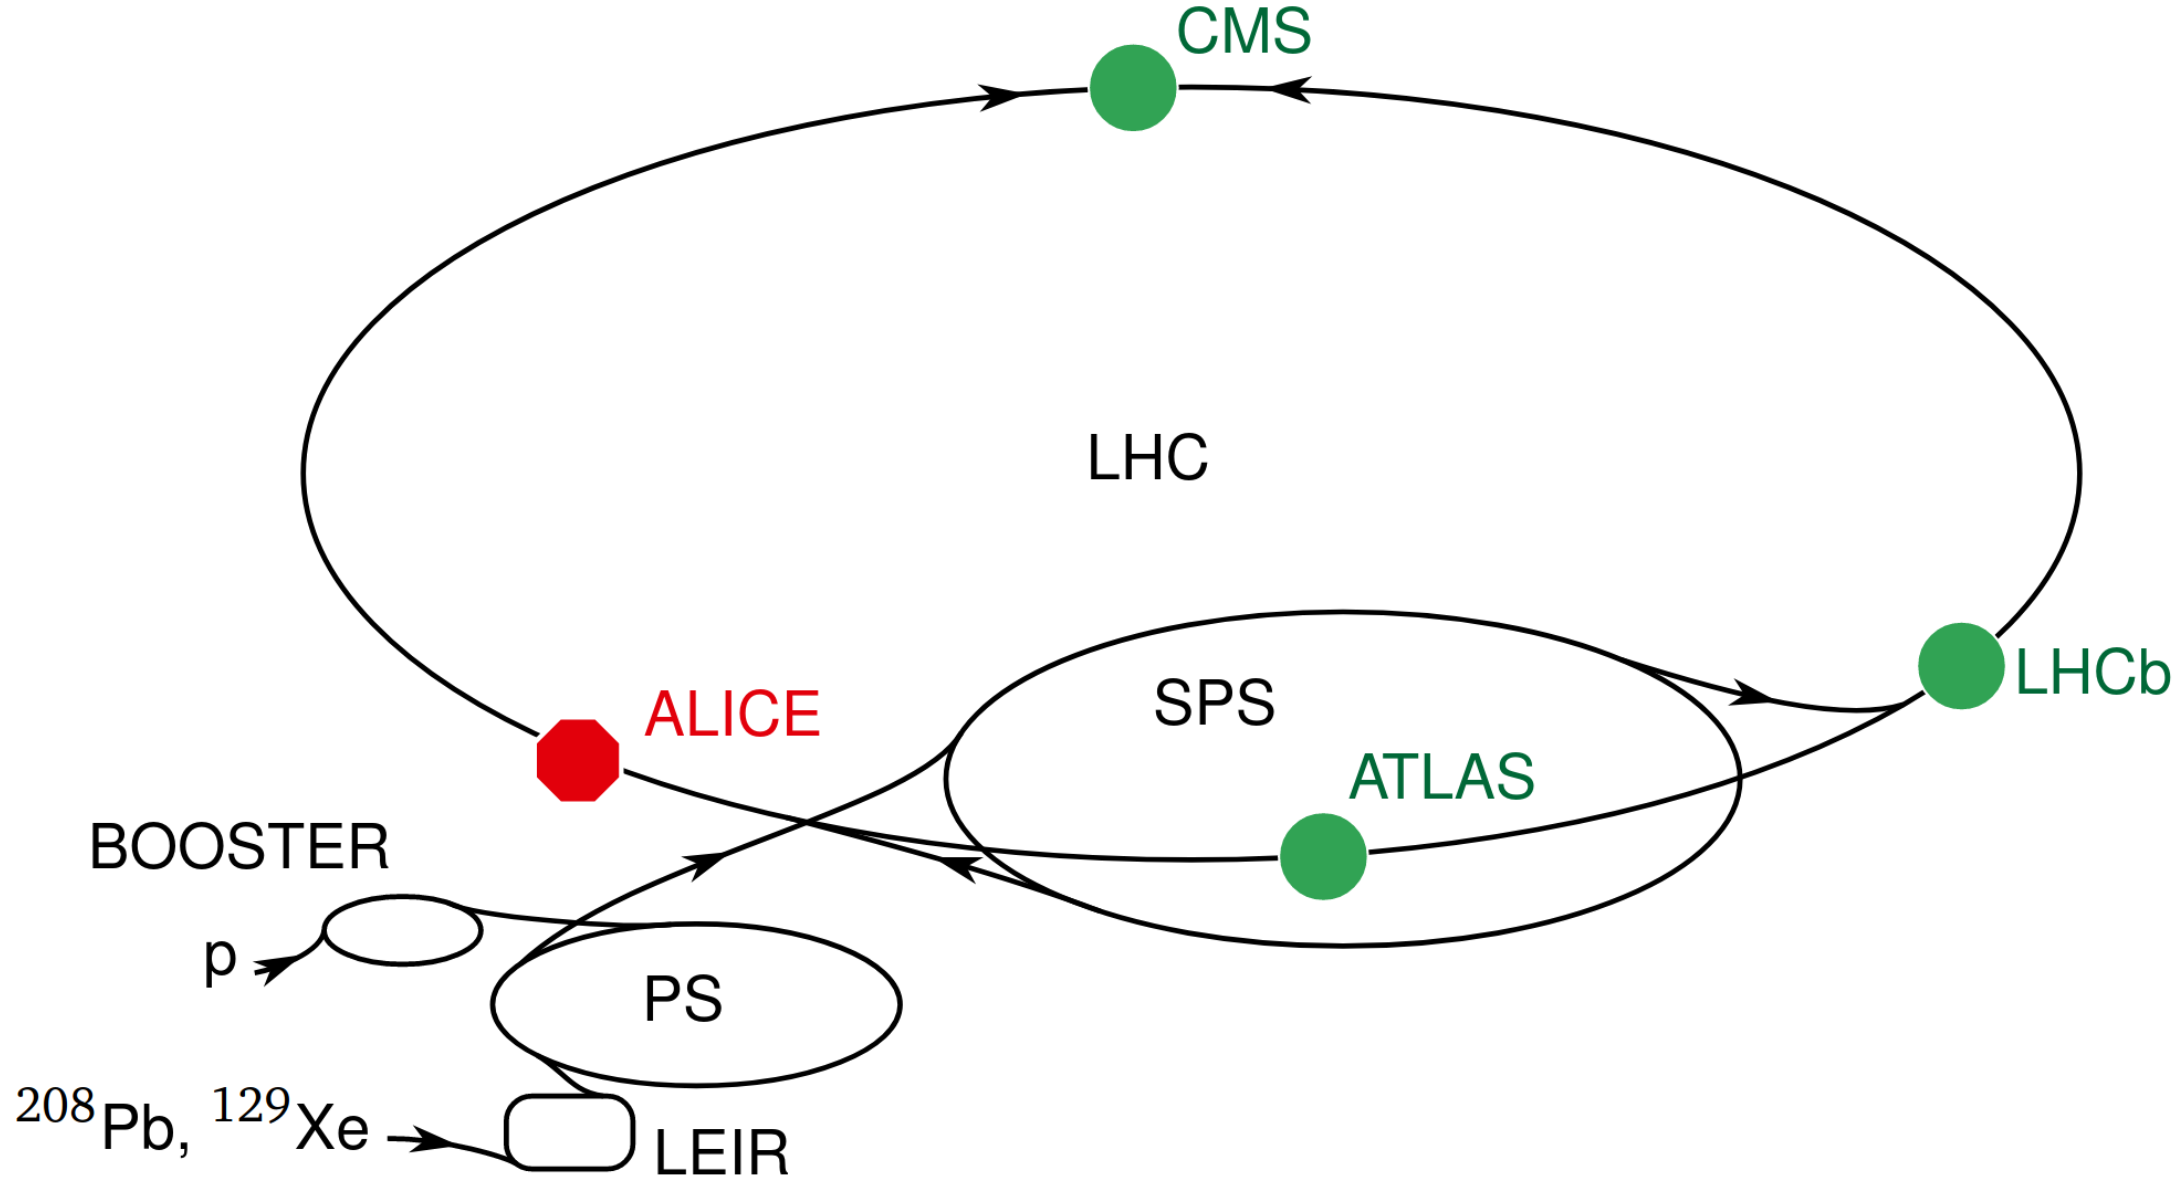
\includegraphics[width=12cm]{Plots/LHC.png}  
\caption{Schematic design of the CERN accelerator complex (cite here).}
\label{LHC}
\end{figure}
\section{ALICE}
%https://home.cern/science/experiments/alice
%"The CERN large hadron collider : accelerator and experiments"
ALICE is dedicated to the study of strong interacting matter at temperatures and densities high enough to presumably create a QGP. Hundreds of physicists from 30 different countries participate in the research of this extreme state of matter as part of the ALICE collaboration. The ALICE experiment is located in the vicinity of St Genis-Pouilly in France and lies 54 m under the ground. It is 26 m long, 16 m high and 16 m wide and consists of 18 different detectors installed in three distinct parts: the central barrel, which is the most relevant part for this work, the forward detectors and the muon spectrometer. \\
%For instance, heavy flavour production and jet fragmentation serve as probe for the parton energy loss in the QGP. Moreover, the geometry of the collision volume is provided by the multiplicity and the transverse or zero-degree energy flow. The equation of state of the QGP as well as transport properties can be studied by means of the elliptic flow, which gives information of the anisotropy of azimuthal momentum space of the particles produced in ultra-relativistic collisions. In addition, quarkonia production represent an important tool for the study of the deconfined state and the parton recombination. Prompt photons probe the thermal radiation of early stages of the collisions.\\
The central barrel is a cylindric structure built around the beam pipe and installed within the solenoid magnet L3, which produces a magnetic field that bends the trajectory of charged particles. The detectors that form the central barrel are, from the inside out, the Inner Tracking System (ITS), the Time Projection Chamber (TPC), the arrays of the Time-of-Flight (TOF) detector, the High Momentum Particle Identification Detector (HMPID), the Transition Radiation Detector (TRD) and three electromagnetic calorimeters (EMCAL, DCAL and PHOS). In Figure \ref{ALICE}, the schematic design of the ALICE experiment is shown. \\
The forward detectors are located at small angles along the beam pipe. The two arrays of the V0 detector are placed on both sides of the collision vertex and they are used mainly to trigger events and determine the centrality in heavy-ion collisions. Furthermore, the Forward Multiplicity Detector (FMD), next to the V0, and the Photon Multiplicity Detector (PMD), mounted on the L3 magnet door, estimate the multiplicities of charged particles and of photons respectively. Finally, on both ends of the beam pipe the Zero-Degree Calorimeters (ZDC) measure spectator nucleons in heavy-ion collisions. \\
In this work, \pt distributions of inclusive charged particles produced in pp collisions as well as in nine centrality Pb-Pb classes are calculated. For this reason, the ITS and the TPC, which are the detectors used for the reconstruction of charged-particles tracks, as well as the V0 detector, required for the centrality estimation, will be discussed in the next sections. 
\begin{figure}[tb!]
\centering
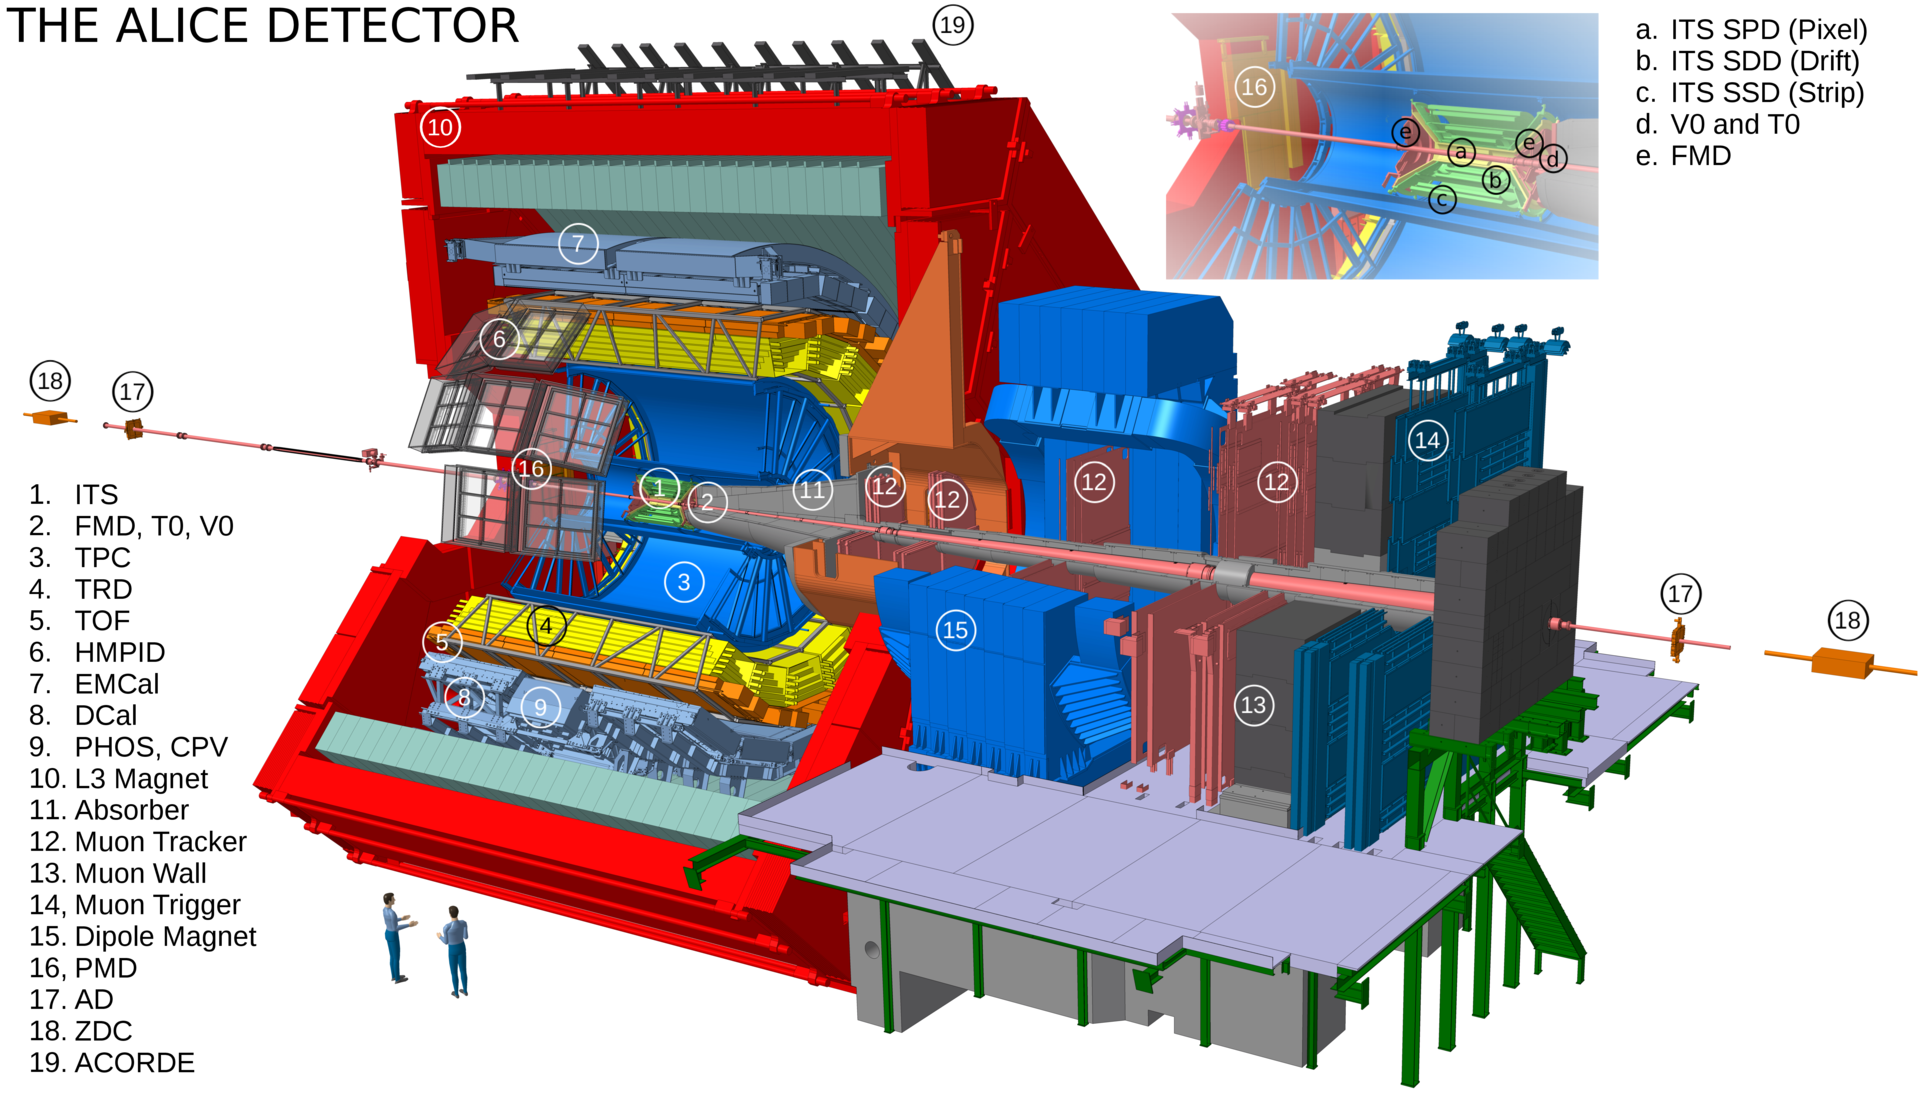
\includegraphics[width=15cm]{Plots/Alice.png}  
\caption{Schematic layout of the ALICE detector (cite Tauro).}
\label{ALICE}
\end{figure}
\subsection{ITS}
%https://cds.cern.ch/record/1071641/files/p143.pdf
The ITS is designed to cover a broad number of applications, making it into one of the most important and versatile detectors of the ALICE experiment. The detector is employed for the reconstruction of charged-particle tracks with low momentum and to particle identification. Moreover, the detector is also used for the primary vertex reconstruction and the location of secondary vertices from decays of hyperons and particles carrying heavy flavour. \\
The detector is located in the immediate surroundings of the beam pipe. The ITS has a pseudorapidity coverage of $|\eta| < 0.9 $ and an overall radius of 51 cm. It is equipped with six layers that built three different subdetectors with radii between 4 and 43 cm. From the inside out, the subdetectors are the Silicon Pixel Detector (SPD), the Silicon Drift Detector (SDD) and the Silicon Strip Detector (SSD).  \\
At LHC energies, the track density and the radiation near the nominal interaction point reach extreme levels. The technical design of the SPD, which corresponds to the two innermost layers of the ITS, is employed to measure the collision vertex in such conditions with high precision. In addition, the SPD can also be used for triggering. The data for the track reconstruction is collected measuring charged carriers that are created when a charged particle traverses the detector volume. \\
The next two layers correspond to the SDD. The layers are capable of measuring the free electrons caused by the ionization of the detector material when the charged particles traverse it. The electrons drift under the influence of an electric field towards the edges of the detector where they are detected. The layers are able to detect multiple tracks at a time. The SDD is also employed for the measurement of the deposited specific energy loss d$E/$d$x$, which is required for the particle identification.\\
The SSD, which comprises the two outer layers of the ITS, is located near to the TPC in order to match smoothly the track points from the respective detectors. The detector is able to provide tracking points in two dimensions as well as specific energy loss information for the identification of particles with low momentum.

\subsection{TPC}
%Unterkapitel, amplification value of 2e4 und MWPC.png: https://www.uni-frankfurt.de/46491136/Generic_46491136.pdf
%ALICETPC.png: "The ALICE TPC, a large 3-dimensional tracking device with fast readout for ultra-high multiplicity event"
The TPC is a hollow cylindric detector filled with a gas mixture (Ne-CO$_2$-N$_2$) and a pseudorapidity coverage of $|\eta| < 0.9 $  that serves as the main tracking device of the ALICE experiment. The detector focuses primarily on a three dimensional reconstruction of tracks, particle identification via specific energy loss and determination of collision vertices. It has an inner radius of around 0.85 m that surrounds the ITS and an outer radius of around 2.5 m, while the length is approximately 5 m along the beam direction. This corresponds to a detector volume of 88 m$^3$. In Figure \ref{ALICETPC}, a schematic representation of the ALICE TPC is shown. \\
When a charged particle traverses the gas mixture of the TPC, electron-ion pairs are created through ionization. The detector volume operates as a field cage which creates a uniform electrostatic field by means of a central high-voltage electrode and two readout chambers located at the opposite endcaps which are used as electrodes. As consequence of the electric field, the freed electrons drift towards the readout planes, into which a two dimensional representation of the track is projected. The measurement of the drift time of the electron provides a third coordinate given that the electrons drift with a constant velocity. This leads a reconstruction of the track in three dimensions. The magnetic field of the L3 magnet, which is parallel to the electric field, bends the trajectory of the tracks such that the momentum of the particle can be calculated by means of the Lorentz force.\\
The two endcaps of the TPC are equipped with multi-wire proportional chambers (MWPC), a type of gas detector which constitute the readout planes of the TPC. A pad plane at ground potential works as the cathode of the detector which is also used as the outer layer of the MWPC. Above the pad plane, three wire planes build the readout chambers. From the outside in, these are a grid of anode wires, a cathode wire plane and a gating grid. A sketch of a MWPC is given in Figure \ref{MWPC}. \\
The anode, at positive high voltage, and the cathode, at ground potential, contain the amplification region. Here, the drifted electrons originated in the TPC volume move under the influence of an electric field which increases with the distance from the anode wires. When the voltage surpasses a certain threshold, electrons carry sufficient energy to ionize atoms through collisions, which causes a cascade of more free electrons that in turn ionize more atoms. This leads to an avalanche effect that amplifies the initial signal by a factor of $2$x$10^4$ (cite commissioning TPC). The drift and amplification regions are separated by the gating grid. This instrument remains open after the triggering of an event and during the drift time that an electron needs over the full TPC length. The gating grid is closed otherwise to prevent ions from drifting to the TPC volume and by that causing field distortions.
\begin{figure}[tb!]
\centering
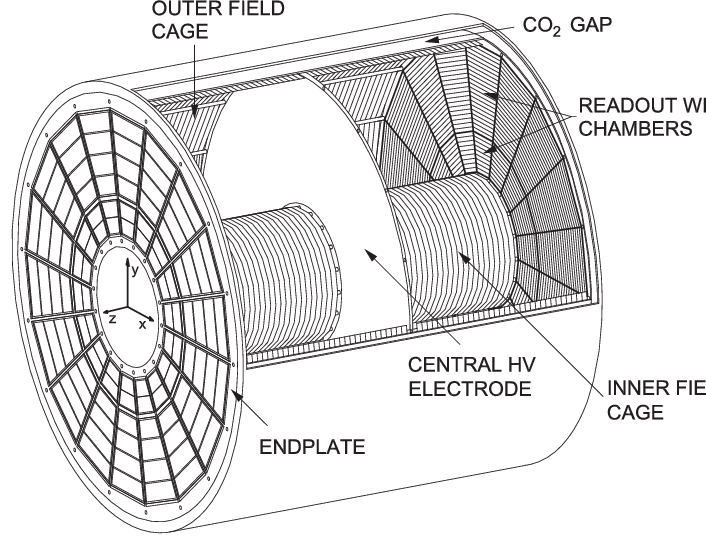
\includegraphics[width=11cm]{Plots/ALICETPC.png}  
\caption{Schematic design of the ALICE TPC (cite link).}
\label{ALICETPC}
\end{figure}
\begin{figure}[tb!]
\centering
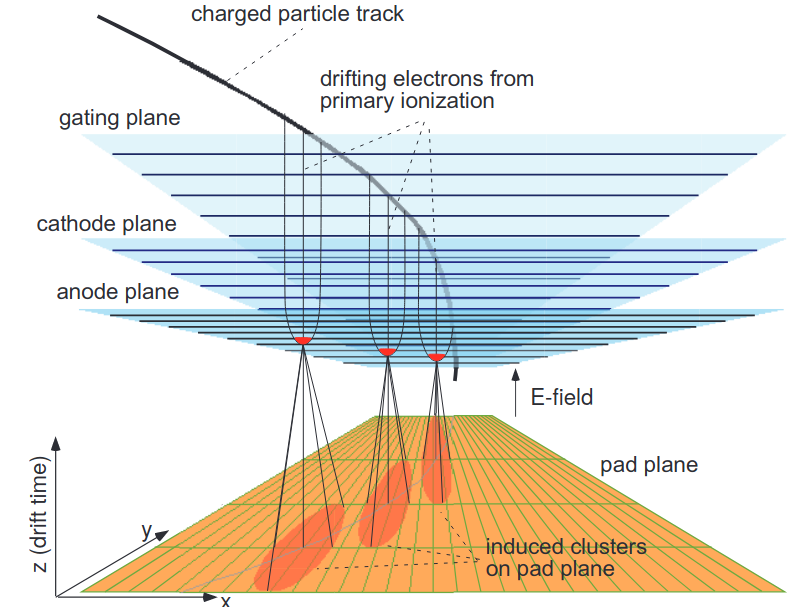
\includegraphics[width=9cm]{Plots/MWPC.png}  
\caption{Schematic design of a multiwire proportional chamber (cite Jens).}
\label{MWPC}
\end{figure}
\subsection{V0 detector}
The V0 detector is comprised of two circular arrays of scintillator counters, called V0A and V0C, which are located on both sides of the ALICE interaction point. The V0A array is installed at 3.29 m away from the collision point along the beam direction, while the V0A is placed at 0.88 m away in opposite direction. The arrays cover a rapidity of $2.8 < \eta < 5.1 $ and $-3.7 < \eta < -1.7 $, respectively. The V0 detector is mainly used for trigger the data taking and for the estimation of the centrality in heavy-ion collisions. Given the large trigger rate expected from undesired background signal in pp collisions, the V0 detector is designed to discriminate between collision and background events by means of the signal arrival time. For the data used in this work, the signals in both arrays must be in coincidence to fulfill the trigger condition. The process of the centrality determination will be described at the end of this chapter.
\subsection{Track reconstruction}
\label{trakcrecon}
%track variables per si ho necessites per algo, pero no lhas fet servir: %https://cds.cern.ch/record/2045797/files/Report.pdf
%https://arxiv.org/pdf/1402.4476.pdf
The detectors used for the tracking reconstruction are mainly the ITS and the TPC. The TRD is also employed for the tracking of particles with momenta above 1 GeV/$c$. All detectors involved are specially designed to be able to operate in environments with a high density of tracks such as in the ALICE experiment. The tracking algorithm can be divided in three phases, namely the localization space points, the track finding and the fitting of the trajectory.\\
The tracking procedure starts with the merging of the individual signals in each detector separately in order to form so-called clusters, which are characterized by several parameters such as the position, the signal amplitude, the signal time or the corresponding errors. After the clusterization, paths between pairs of clusters, each of them located in an SPD layer, are determined. The space point where most paths, also called tracklets, converge is designated as the preliminary interaction vertex. This process is iterated several times in order to reduce so-called pile-up events, which are events produced in a bunch crossing different from the one that triggered the data recording. In addition, multiple collisions occurring within the same bunch crossing are also considered pile-up, although this takes place much more rarely. By the iteration of the algorithm, an event is identified as pile-up and removed from the data sample when multiple primary vertices are reconstructed. In case of a missing converging point, this is substituted by the maximum along the beam axis of points of closest approach of tracklets.\\
\begin{figure}[tb!]
\centering
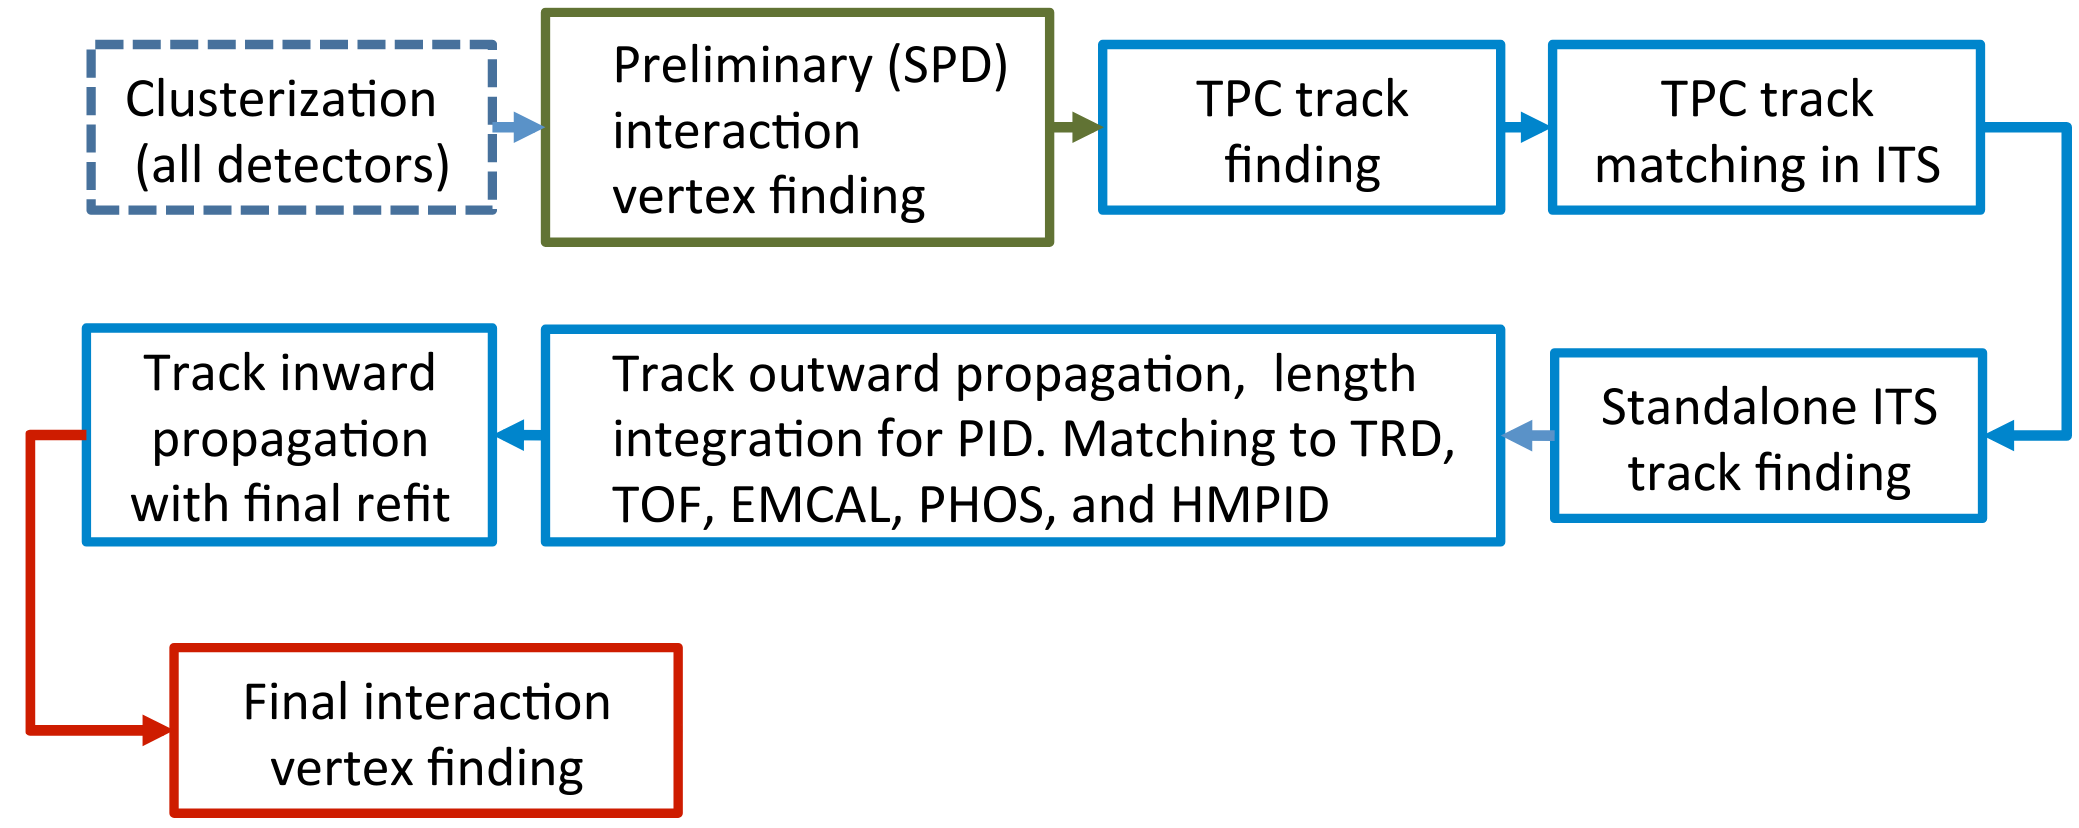
\includegraphics[width=14cm]{Plots/EventRecFlow.png}  
\caption{Schema of the workflow for the track reconstruction algorithm for charged particles in ALICE. (cite performance in ALICE) }
\label{eventflow}
\end{figure}
The track reconstruction is performed in three phases, namely first towards the nominal point in radial direction, then outwards and finally inwards again. In Figure \ref{eventflow}, a schematic representation of the workflow for the track finding is shown. The procedure starts by determining the path through two TPC clusters, beginning with those located at large radii, and the preliminary primary vertex. An analog search is performed using three TPC clusters and without considering the primary vertex. The resulting paths represent the track candidates or seeds. These are propagated inwards to the innermost TPC radii including progressively the clusters along the way that fulfill a proximity criterion, which takes into account the positions and errors. To prevent the algorithm from reconstructing the same tracks several times, a limit for the fraction of shared clusters between pairs of tracks is established (see Section \ref{TrackSelection}).\\
Next, the tracking continues in the SSD using as starting point the TPC seeds. Analogous to the reconstruction in the TPC in two steps, the seeds are propagated inwards to the SPD ITS updating the seed with clusters at each ITS layer that fullfill the proximity criterion. If no clusters are found, the track is flagged with the test statistic $\chi^2$ for poor quality. This is considered later in the track selection (see Section \ref{TrackSelection}). \\
In the process, each TPC seed produces in the ITS a tree of potential tracks. If shared clusters are found among the candidates with the highest quality based on the $\chi^2$, other candidates are selected in the corresponding trees. Tracks with low momenta are occasionally absorbed by the detector material before entering the TPC, which results in a low reconstruction efficiency in this range. As result, some TPC tracks can not be connected with ITS clusters. To solve this, tracks with such a momentum are determined in a standalone ITS reconstruction with clusters from the three innermost ITS layers and the preliminary primary vertex. These seeds are propagated outwards taking into account the proximity cut. Finally, the resulting track candidates are refitted using a technique called Kalman filter (cite here.Hallo Mario, was geht ab. Dieser letzte Teil ist für tracks mit einem \pt von max. 80MeV. Brauche ich das zu erwähnen der Vollständigkeits halber?)\\
After the standalone ITS track finding, an extrapolation of all tracks is performed to their point of closest approach to the preliminary primary vertex. Then, the tracks are refitted by means of the Kalman filter outwards up to the utmost radii of the TPC. At each cluster, track parameters are updated and stored for the later particle identification with TOF. The tracks are propagated through the rest of the detectors of the central barrel in an attempt to match the signals. The extracted information is not used to modify the track parameters, but for particle identification. Finally, the resulting tracks are propagated and refitted once again starting from the outer radii of the TPC up to the SPD. In this process, the final track parameters, such as the track position or the inverse of the radius among others, and the corresponding errors are stored. Once the reconstruction is completed, global tracks are used to optimize the position of the primary vertex determined before with SPD tracklets. This is achieved with an extrapolation of the tracks to the point of closest approach along the beam axis. By that, an important track variable, the so-called distance of closest approach (DCA), is calculated as the distance of the primary vertex to the nearest track point. 
\subsection{Transverse momentum and momentum resolution}
\label{ptandmomreso}
The trajectory of a charged particle traveling through the TPC is characterized by a helical form caused by the prevailing magnetic field. This is caused by the Lorentz force which relates the radius $r$ of the track curvature with the transverse momentum \pt of the particle. Thus, the transverse momentum of a track can be calculated via:
\begin{equation}
p_\text{T} = r \cdot e\cdot B
\label{radius}
\end{equation}
where $B$ is the magnetic flux density perpendicular to the particle of charge $e$. In practice, the measurement of this radius is demanding since even particles with low transverse momenta present radii that far exceed the outer radius of the TPC. For this reason, the radius is substituted by another quantity which parametrizes the track curvature and which can be measured within the detector volume. This is the so-called sagitta (see Figure \ref{Sagitta}), an arc parameter which is inverse proportional to the radius of the track for the extreme case of a chord $L \ll r$ spanning the base of the arc (cite here):
\begin{equation}
s = \dfrac{l^2}{8r}
\end{equation}
Therefore, we obtain for $B$ given in T, $L$ in m and \pt in GeV/$c$ (cite here)
\begin{equation}
s = \dfrac{0.3e \cdot B \cdot l^2}{8p_\text{T}}
\end{equation}
\begin{figure}[tb!]
\centering
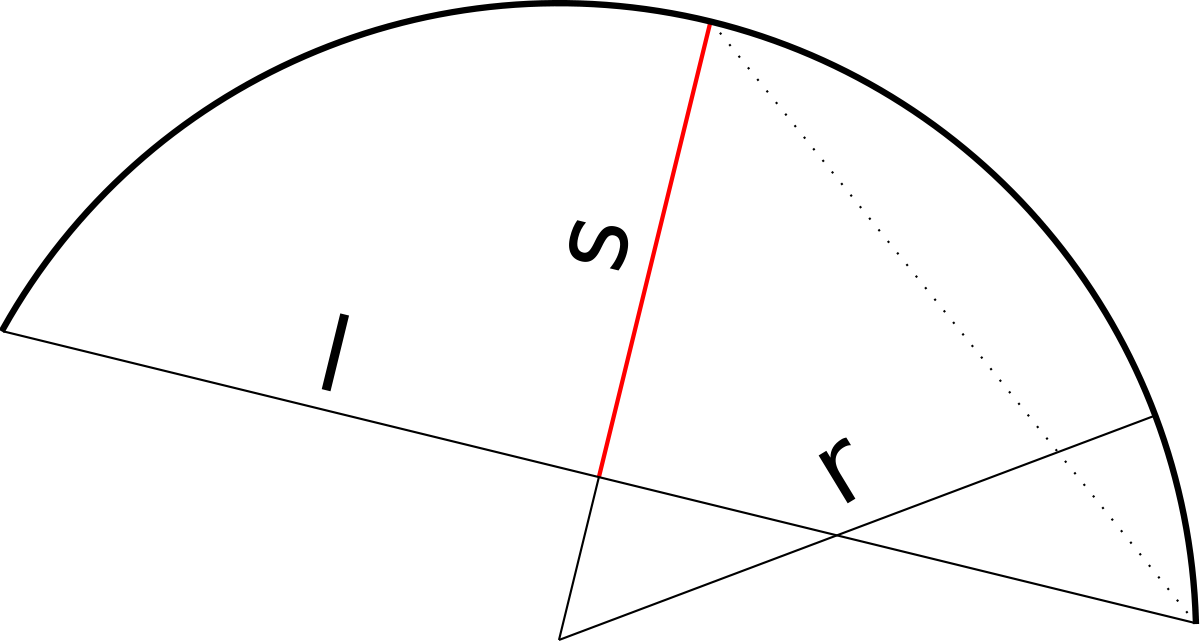
\includegraphics[width=7cm]{Plots/Sagitta.png}  
\caption{Visualisation of the radius $r$, the sagitta $s$ and the chord $l$ of a circular arc (cite wikipedia).}
\label{Sagitta}
\end{figure}
\hspace{-0.25cm} The sagitta is measured with an uncertainty due to the spatial resolution of the detectors which in turn implies that the resulting inverse of the transverse momentum is affected by an uncertainty $\sigma(1/p_\text{T})$. It can be then shown that the relative transverse momentum resolution $\sigma(p_\text{T})/p_\text{T}$ can be approximated by (cite knichel):
\begin{equation}
\dfrac{\sigma(p_\text{T})}{p_\text{T}} \approx p_\text{T} \cdot \sigma(1/p_\text{T})
\label{equationRelSigma}
\end{equation}
\subsection{Centrality estimation}
%https://arxiv.org/pdf/1301.4361.pdf
%Henner Skript
%BA Gabriel
\label{centEstim}
The volume of the interaction region in AA collisions depends on the distance perpendicular to the beam axis between the centers of the colliding nuclei, the so-called impact parameter $b$. This leads to the definition of an observable, the centrality, that characterizes the overlap between two nuclei in a collision event and, therefore,  which depends on the impact parameter. A distinction in centrality intervals or classes can be made taking into account the size of the overlap region. Thus, head-on collisions are referred to as central, while those collisions in which nuclei have a minimal contact are called peripheral. The inbetween centrality classes are denominated semi-central. The centrality is given as a percentage of the total geometric cross section, \\
In this context, nucleons of colliding nuclei are classified in participants or spectators depending on whether they take part in the collision or not. The number of participants $N_\text{part}$ in a collision determines the number of binary collisions $N_\text{coll}$. The relation between these geometrical quantities with the impact parameter is described by a technique called Glauber Model (cite here), in which colliding nuclear are presented as a superposition of binary nucleon-nucleon collisions. The nucleon density distribution is assumed to follow a Woods-Saxon potential (cite here). The model also defines a new observable, which quantifies the number of ancestors $N_\text{ancestors}$ in a collision, i.e. emitters of particles. This quantity is calculated with $N_\text{ancestors} = f \cdot N_\text{part} + (1 - f)\cdot N_\text{coll} $, where $f$ represents a free parameter. This is based on two-component models, which assumes that soft processes are responsible for the production of an average multiplicity proportional to $N_\text{part}$, while hard processes escalate with increasing $N_\text{coll}$. Since none of these observables can be measured experimentally, the estimation of the centrality must be based on another measurable quantity, namely the charged-particle multiplicity $N_\text{Ch}$, which is assumed to fall monotonically as function of the impact parameter.\\ % the energy $E_\text{ZDC}$ that particles deposit in the ZDC, which is inversely proportional to the number of spectators. 
The centrality is estimated using as input the multiplicity distribution measured with the deposited energy in the V0 detectors. The measured multiplicity is parametrized with a negative binomial distribution (NBD) (cite here), which is capable of reproducing it accurately. To this end, a Glauber Monte Carlo simulates $N_\text{part}$ and $N_\text{coll}$ values given an impact parameter $b$. The number of produced particles per interaction is calculated with a NBD that provides the probability $P_{\mu,k}(n)$ for the production of $n$ particles per ancestor, where $\mu$ is the mean multiplicity per ancestor and $k$ parametrizes the width of the $N_\text{ch}$ distribution. The Glauber Monte Carlo simulates collision events. From the corresponding geometries, $N_\text{part}$ and $N_\text{coll}$ values are inferred for each of events, which in turn, leads to the determination of $N_\text{ancestors}$. Next, a NBD is parametrized over all $N_\text{ancestors}$ in an event by adjusting the parameters $\mu$, $k$ and $f$ in order to minimize the test statistic $\chi^2$ of the fit. This allows to simulate the averaged V0 amplitude for the corresponding event. Figure \ref{V0Amplitude} shows as example the distribution of the amplitudes in the V0M array parametrized with a NBD-Glauber fit in Pb-Pb collisions at a centre-of-mass energy $\sqrt{s_\text{NN}}= 5.02$ TeV. In the figure, the centrality classes are also given, whose determination is explained below. The distribution presents a peak that corresponds to the peripheral collisions, while the plateau covers the region of semi-central collisions and the edge the interval of central collisions. The edge at maximum amplitude is explained by fluctuations of $N_\text{part}$ and d$N_\text{ch}$d$\eta$ and by the acceptance and resolution (cite paper).\\
It is worth mentioning that the V0 amplitude is contaminated with events from electromagnetic interactions due to the high cross section for these process at LHC energies. Such events are related to very small multiplicities, which results in a contamination of the V0 amplitude in this range. Other phenomena at such multiplicities as for example inaccuracies in the triggering or beam gas collisions also represent contributions to the contamination. Nevertheless, the Glauber Model is designed to describe exclusively hadronic interactions. This fact explains the better agreement of the NBD fit with data at mid and high multiplicities. In this context, the centrality classes are determined by defining an upper bound for the range in which the measurement is not biased, to which the estimation of the centrality classes is anchored. This is the so-called anchor point, which in case of ALICE is established at 90\%. The centrality classes are derived then taking into consideration the NBD parametrization.
\begin{figure}[tb!]
\centering
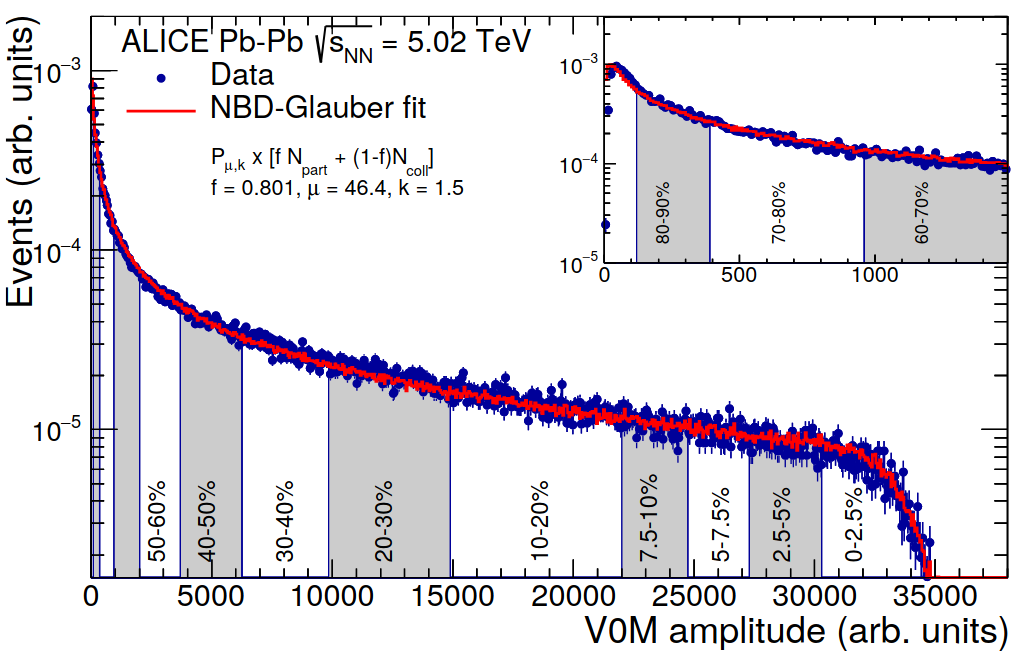
\includegraphics[width=12cm]{Plots/V0Amplitude.png}  
\caption{Multiplicity distribution measured with the V0M array and parametrized with a NBD-Glauber fit. Centrality percentiles are also represented.}
\label{V0Amplitude}
\end{figure}
\chapter{Analysis}
Since its theoretical proposal forty years ago, the QGP has been a subject of huge interest in the field of high-energy physics, given that it could offer answers to fundamental questions about the structure of matter. The ALICE experiment at the LHC is dedicated to the study of this exotic state of matter that is believed to form in ultra-relativistic heavy-ion collisions. \\
As discussed in the first chapter of this work, the physics of strongly interacting matter can be investigated by means of the nuclear modification factor $R_\text{AA}$ which compares the yield of inclusive charged particles in AA collisions and a corresponding reference measurement in pp collisions. In this chapter, an analysis of transverse momentum distributions in Pb-Pb and in pp collisions at a centre-of-mass energy $\sqrt{s_\text{NN}}= 5.02$ TeV measured with ALICE is presented. First, the selected data samples are detailed. Then, the procedures to correct for detector effects which have an impact on the \pt distributions are described. With these corrected \pt distributions the nuclear modification factors are calculated. The results are discussed and compared to previous ALICE measurements (cite paper here).
\section{Data sample}
\begin{table}[tb!]
\centering
\renewcommand{\arraystretch}{1.5}
\begin{tabular}{c|c|c|c}
\toprule
\rowcolor{headerBlue} \textbf{System} & \textbf{statistics}  \textbf{(M)} & \textbf{MC generator} &  \textbf{MC statistics } \\
\midrule
             & 560 (FAST) & & \\
\textbf{pp}	 &	 &   PYTHIA + GEANT3  & 25\%  	 \\
 &  318 (CENT)   &  	\\
\hline
\textbf{Pb-Pb} & 110 &  HIJING + GEANT3  & 2\% \\
				 &	   & 		 \\
\bottomrule
%pp FAST und PbPb values token from: https://twiki.cern.ch/twiki/bin/view/ALICE/AliDPGReconstructedDataTakingPeriodsSummary
%pp CENT token from Run Condition Table https://alimonitor.cern.ch/configuration/index.jsp?partition=LHC17p&pass=1&raw_run=&filling_scheme=&filling_config=&fillno=&energy=&intensity_per_bunch=&mu=&interacting_bunches=&noninteracting_bunches_beam_1=&noninteracting_bunches_beam_2=&interaction_trigger=&rate=&beam_empty_trigger=&empty_empty_trigger=&muon_trigger=&high_multiplicity_trigger=&emcal_trigger=&calibration_trigger=&quality=&muon_quality=&physics_selection_status=&comment=&field=&det_aco=&det_ad0=&det_emc=&det_fmd=&det_hlt=&det_hmp=&det_mch=&det_mtr=&det_phs=&det_pmd=&det_spd=&det_sdd=&det_ssd=&det_tof=&det_tpc=&det_trd=&det_t00=&det_v00=&det_zdc=&hlt_mode=&changedon=
\end{tabular}
\caption{Overview of the used data taking periods, the approximate number of events contained in them and the MC productions they are associated with including the percentage of simulated statistics.}
\label{tab:Periods}
\end{table} 
This thesis will make use of pp and Pb-Pb collisions at $\sqrt{s_\text{NN}}= 5.02$ TeV recorded by ALICE in the years 2017 and 2018 respectively. For the pp data takings, the interaction rate was 50 kHz, while in Pb-Pb it was 7.5 kHz. Furthermore, for each data taking period there is at least one MC production, which simulates the exact same conditions and technical specifications of the detector at the time of data taking, anchored to it. The particle collisions for the MC productions were generated by PYTHIA (cite here) in the case of pp collisions and by HIJING (cite here) for the Pb-Pb collisions, while the corresponding detector response was simulated by GEANT3 (cite here). The limited computing time available for these simulations allows to cover only a percentage of the total statistics present in data. An overview of the number of events contained in each data set is summarized in Table \ref{tab:Periods}. The number of events was measured after the event selection depicted in the following section of this chapter.\\
The examined pp data consists of two separated subsets that differ by their the readout configuration: the first data subset corresponds to collisions measured excluding the detector signal of the SDD layers, which in this thesis will be referred to as \textit{FAST} in accordance with ALICE convention. The exclusion of the signal occurs whenever the SDD is inoperable due to its dead time. In contrast, the collisions in the second data subset were reconstructed including the information of the SDD layers. These collisions are labeled as \textit{CENT}. Furthermore, the events of the \textit{CENT} subset were reconstructed also without the SDD information allowing to study the impact of the absence of the SDD layers during the tracking. This allows to compare any observable extracted from \textit{CENT} with SDD and from \textit{CENT} without SDD data. \\
As shown in Table \ref{tab:Periods}, the \textit{FAST} subset contains almost three times as many events as \textit{CENT}. In this work, these two data takings are combined in order to make use of all measured pp collisions. In the big picture, this increase of statistics will lead to an enhanced precision in the high \pt region and to an enlarged \pt reach of the charged-particle \pt spectrum in pp collisions. Such an improvement will in turn be reflected in the nuclear modification factors. 
%https://arxiv.org/pdf/1402.4476.pdf Performance of the ALICE Experiment at the CERN LHC
\section{Trigger and event selection}
\subsection{Trigger}
During the data taking, a trigger decides in real time whether a collision candidate is worth to be stored or not. The ALICE experiment focuses its research activities on the investigation of strongly interacting matter and therefore inelastic collisions are of particular interest. Moreover, the trigger is also designed to reject undesired beam-gas interactions. \\
The trigger configuration which imposes the smallest bias and thus accepts the majority of the overall inelastic cross section is called minimum bias (MB) trigger. For the data sets used in this thesis, a MB trigger that requires signals both in the V0A and V0C detectors in coincidence with the bunch crossing (V0$_\text{and}$) (cite "Performance of ALICE", s. 22) is used.
\subsection{Selection of events}
\begin{figure}[tb!]
\centering
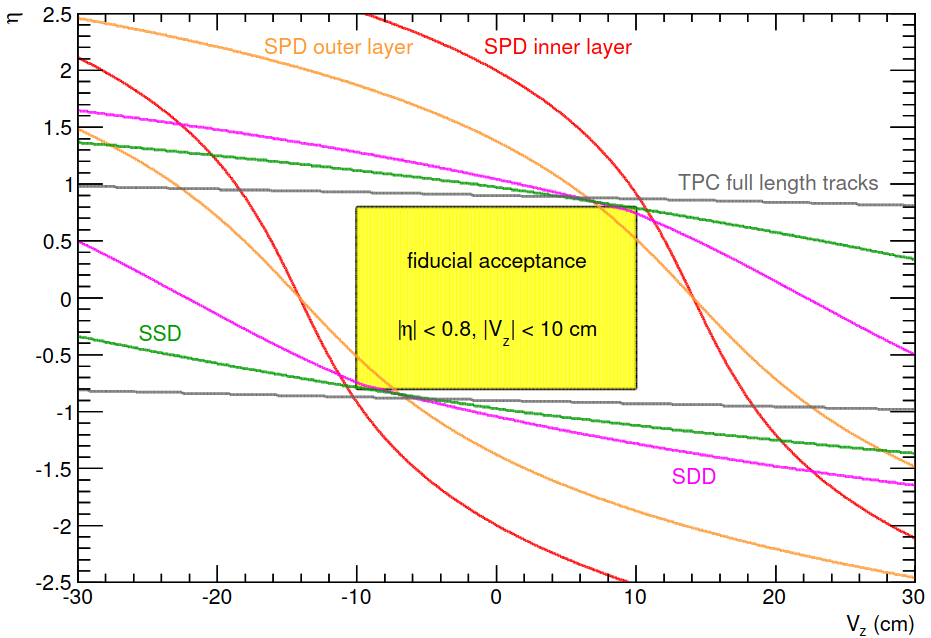
\includegraphics[width=12cm]{Plots/fiducialAcc.png}  
\caption{Pseudorapidity acceptance of the SPD, the SDD, the SSD and the TPC shown as function of the position of the primary vertex along the $z$-axis. The fiducial acceptance represents the region where most tracks can be reconstructed (cite mknichel).}
\label{fiducialAcc}
\end{figure}
In an offline stage of the event selection, collision candidates that satisfy the trigger condition undergo a selection process in order to reduce the contamination with poor quality events. A part of this contamination corresponds to a background signal originated from interactions of the beams with the machine. This beam background is discriminated mainly by means of the signal arrival time of the events in the V0 modules. The arrival time of background events is shorter than the one of a collision produced in the nominal interaction point. This difference is exploited to exclude background events from the data sample. \\
The pseudorapidity acceptance of the ALICE tracking detectors depends on the position of the primary vertex $\text{V}_z$ along the beam axis $z$ as illustrated in Figure \ref{fiducialAcc} for the ITS subdetectors and the TPC. To ensure a symmetric pseudorapidity coverage of $|\eta| < 0.8$, the vertex position was restricted to $|V_z| < 10$ cm.
%https://arxiv.org/pdf/1402.4476.pdf
%https://arxiv.org/pdf/1110.5530.pdf
%https://indico.cern.ch/event/752367/contributions/3116617/attachments/1704565/2858687/DPG_AnalysisTutorial_20181129.pdf
\section{Track selection}
\label{TrackSelection}
\begin{table}[tb!]
\renewcommand{\arraystretch}{1.5}
%\rowcolor{bodyBlue}
\centering
\begin{tabular}{l c}
\toprule
\rowcolor{headerBlue}  \textbf{Track variable} &  \textbf{Condition} \\
\midrule
\multicolumn{2}{c}{\textbf{Selection of primaries}} \\
\midrule
$\text{DCA}_{z}$ & $\leq 2 $ cm\\
$\text{DCA}_{xy}$ & $\leq 7\sigma$ \\
\midrule
\multicolumn{2}{c}{\textbf{ITS selection}} \\
\midrule
at least one hit in the SPD & required \\
ITS refit &  required\\
$\chi^2$ per ITS cluster  & $< 36$ \\
\midrule
\multicolumn{2}{c}{\textbf{TPC selection}} \\
\midrule
TPC refit &  required\\
$\chi^2$ per TPC cluster (pp collisions) & $< 4$ \\
$\chi^2$ per TPC cluster (Pb-Pb collisions) & $< 2.5$ \\
fraction of shared  TPC clusters&  $<  0.4$\\
ratio of crossed rows over findable clusters  & $> 0.8$ \\
geometric length (TPC dead zone) & $3$ cm  \\
geometric length (track length) & $130$ cm \\
\midrule
\multicolumn{2}{c}{\textbf{TPC-ITS selection}} \\
\midrule
$\chi^2$ TPC constrained track vs. global track  & $\leq 36$ \\
\bottomrule
\end{tabular}
\caption{Standard track selection criteria used for analysis of primary charged particles in ALICE.}
\label{tab:Cuts}
\end{table}
Primary charged particles traverse the TPC-ITS detector system describing a trajectory or track which can be reconstructed by means of the procedure detailed in Section \ref{trakcrecon}. These tracks must fulfil several requirements which aim to select good resolution tracks and reduce the contamination from secondary particles present in the data sample. Over the years, the track selection criteria or track cuts have been refined by several analyses on the charged-particle production in ALICE, such as (cite theses), and, as result, the standard track selection listed in Table \ref{tab:Cuts} was established. The same track cuts are implemented in both collision systems pp and Pb-Pb for tracks measured in the kinematic range $p_\text{T} > 0.15\text{ GeV}/c$ and $|\eta| < 0.8$, in data as well as in in the corresponding MC productions. 
\iffalse
\subsection{Selection of primaries}
\label{sec:SelOfPrim}
The distance-of-closest approach (DCA) of a track to the primary vertex, introduced in Section \ref{trakcrecon}, becomes a valuable variable in the supression of secondary particles, which by definition tend to have much larger values than primary particles. For this reason, secondary particles can be removed by setting boundaries to the DCA. In this regard, the standard track selection limits the DCA in beam direction to $2$ cm.\\
With a more aggressive cut, the DCA is also restricted in radial direction by requiring seven standard deviations of the impact parameter resolution, which represents the uncertainty on the DCA to the beam line: %https://indico.cern.ch/event/96989/contributions/2124495/attachments/1114189/1589705/WellsTracking.pdf https://s3.cern.ch/inspire-prod-files-6/6d5c8f5045f30cb63ff7d99fe1a0c79f
\begin{align}
\begin{split}
\text{DCA}_{xy} &\leq 7 \cdot \left(26 + \dfrac{50}{(p_{T}[\text{GeV}/c])^{1.01}}\right) \mu \text{m} \\
& = 7\cdot \sigma
\end{split}
\end{align}
Here, it can be observed that the DCA$_{\text{xy}}$ cut gets more limited the larger the transverse momentum. 
\subsection{ITS selection}
Both mentioned DCA cuts and therefore the selection of primaries are accomplished by virtue of the good DCA resolution achieved by imposing that particles must hit at least one time in the SPD, the innermost layers of the ITS, in order to be selected. Additionally, the ITS refit criterion provides that at least one hit more takes place in one of the ITS layers. \\
A part from that, the ITS track selection has to take also into account the statistical deviation between the reconstructed global track and the fit resulting from reference points from the ITS. This deviation points out that some clusters are assigned to the track incorrectly, which causes a  deterioration of the \pt resolution at high $p_\text{T}$. To prevent that, a statistical variable that evaluates the extent of the deviation named, chi-square, will be limited to $\chi^2$/cluster $< 36$.
\subsection{TPC selection}
Track requirements regarding a refit and a $\chi^2$/cluster cut are also applied in the TPC selection. The TPC refit is implemented using the track reconstruction algorithm twice: from the inside out and in reverse. Further, the $\chi^2$ per TPC cluster is required to stay below a threshold of $4$. \\
The TPC selection focuses also on the detection of fake tracks and tracks that are unintentionally reconstructed multiple times by studying the number of clusters shared by apparently more than one track. These contaminated tracks are excluded adjusting a maximum value for the ratio of shared clusters to all clusters to $0.4$.\\
As already discussed, the clusterization allows the track reconstruction. Since some rows are unable to detect a track due to detector efficiency effects, the number of crossed rows differs frequently from the number of clusters. To correct that, the number of crossed rows includes also those pad rows whose adjacent sides do detect it. Moreover, pad rows that are classified as possible clusters on the basis of the geometry of the track are called findable clusters, a variable more comprehensive than the number of clusters. In this analysis, the ratio of crossed rows over findable clusters must exceed a value of $0.8$. \\
The TPC selection makes a requirement also in relation to the geometric length of the track $L(p_\text{T})$ which is given expressed in cm by:
\begin{equation}
L(p_\text{T}) \geq A - p_\text{T}^{-b}
\end{equation}
where $A=130 \text{ cm}$ corresponds to the minimum length in the active volume of the TPC, $p_\text{T}$ the transverse momentum of the track given in units of $\text{GeV}/c$ and $b=-1.5$ the slope dependency. This calculation excludes the pads situated approximately $3\text{ cm}$ from the sector edges. Furthermore, the geometric track length provides the requirements for the minimum number of crossed rows and of clusters, respectively $0.85\cdot L(p_\text{T})$ rows and $0.7\cdot L(p_\text{T})$ clusters.
\subsection{TPC-ITS selection}
It has been observed that ITS clusters are assigned on occasions improperly to tracks. In further, some tracks can scatter with detector material between the ITS and the TPC. These two effects can result in distortions of the yield	at high $p_\text{T}$. This is prevented through a statistical evaluation between the global track and the constrained track resulting from the TPC information and the primary vertex. The inclusion of the primary vertex can also contribute to a mitigation of the contamination by secondary particles. The statistical evaluation is conducted by means of the $\chi^2_\text{TPC-ITS}$ obtained from the track parameters and their respective uncertainties. Thereby, tracks that exhibit $\chi^2_\text{TPC-ITS}>36$ are rejected.
\fi
\section{Corrections}
After implementing the event and track selections, the uncorrected \pt dependent distributions of the produced charged particles in pp and Pb-Pb collisions can be calculated as shown in Figure \ref{uncorrSpec}. In the case of heavy-ion collisions, the \pt distributions are divided into nine centrality classes. The vertical error bars represent the statistical uncertainties.\\
These \pt distributions are influenced by several detector effects that must be corrected. To this end, most of the corrections are implemented using information provided by MC simulations. In addition, data-driven approaches are used to correct for imperfections of these simulations. \\
\begin{figure}[htb!]
\centering
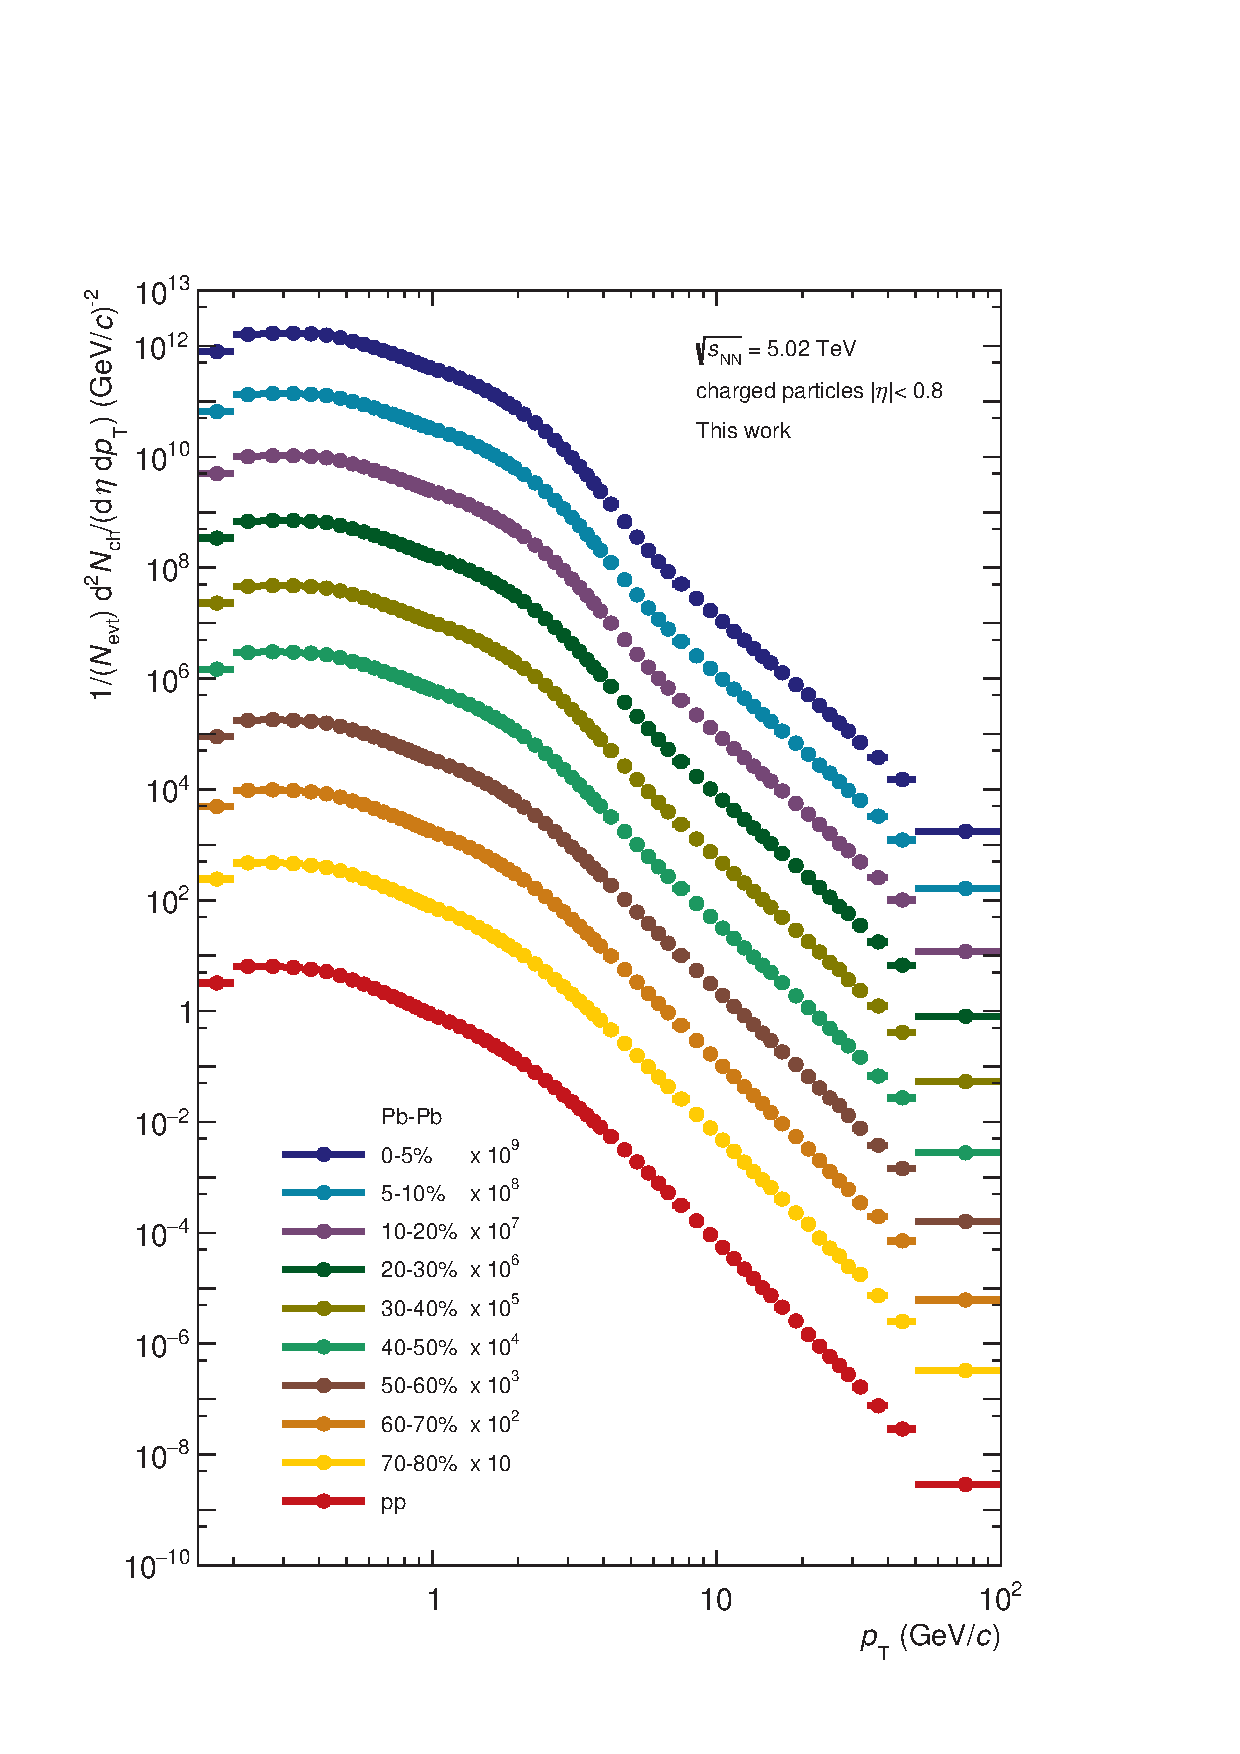
\includegraphics[width=13cm]{Plots/uncorrectedSpectra.pdf}  
\caption{Uncorrected transverse momentum distributions of primary charged particles produced in pp and Pb-Pb collisions at $\sqrt{s_\text{NN}} = 5.02$ TeV. The latter are divided into nine centrality classes. The \pt spectra of Pb-Pb collisions are scaled with a logarithmic factor for a better visibility.}
\label{uncorrSpec}
\end{figure}
Two groups of corrections can be defined according to the level at which they operate, namely event-level corrections, which affect the shift of the spectrum, and track-level corrections, which are \pt dependent and condition consequently the shape of the spectrum. In the following sections, the source of the effects that distort the \pt distributions as well as the corrections applied will be discussed.
\subsection{Overall normalisation}
\label{Norm}
\begin{table}[H]
\centering
\renewcommand{\arraystretch}{1.5}
\begin{tabular}{|c|c|}
\toprule
\rowcolor{headerBlue}  \textbf{Trigger} $\boldsymbol \epsilon_\text{Trig}$ &  \textbf{Vertex reconstruction} $\boldsymbol \epsilon_\text{Vz}$\\
\hline
75.25\%	&	98.48\%		 \\
\bottomrule
\end{tabular}
\caption{Trigger and event vertex reconstruction efficiencies for pp collisions at $\sqrt{s} = 5.02$ TeV recorded with ALICE in 2017.}
\label{tab:effs}
\end{table} 
The number of events $N_\text{ev}^\text{rec}$ that passed the selection criteria and which is used for the normalisation of the \pt distributions does not include some inelastic events that were not triggered or reconstructed. These two phenomena are corrected by means of the so-called trigger efficiency $\epsilon_\text{Trig}$ and the vertex reconstruction efficiency $\epsilon_\text{Vz}$:
\begin{equation}
N_\text{ev}^\text{rec} = N_\text{INEL}\cdot \epsilon_\text{Trig} \cdot \epsilon_\text{Vz}
\end{equation}
where $N_\text{INEL}$ represents the true number of inelastic events. In heavy-ion collisions, both trigger and vertex reconstruction efficiency have been observed to be unity in the studied centrality interval of 0-80\% (Pb-Pb paper). However, the bias has a notable influence in pp collisions. The determination of the respective efficiencies in pp collisions is described below.
\subsubsection{Trigger efficiency}
%cite ALICE 2017 luminosity determination for pp collisions at
%cite vdM:http://cds.cern.ch/record/296752/files/196800064.pdf
%cite value vis. cross section: https://twiki.cern.ch/twiki/bin/viewauth/ALICE/Eventnormalization
%cite MC glauber predictions: https://arxiv.org/pdf/1710.07098.pdf
The MB condition of the ALICE trigger system is able to measure a significant percentage of the total inelastic cross section, yet this measurement is limited due to the efficiency of the trigger $\epsilon_\text{Trig}$. This efficiency connects the visible and the total inelastic cross section as follows:
\begin{equation}
\epsilon_\text{Trig}  =  \dfrac{\sigma_\text{vis}}{\sigma_\text{INEL}} 
\label{effTrig}
\end{equation}
For each data taking period, the visible cross section is measured by determining the luminosity of the experiment, a quantity that evaluates the number of particle collisions and which is measured in events per time per area. To this purpose, a technique called van-der-Meer scan is used, in which the two particle beams are displaced with respect to each other in the transverse directions and the rate of interactions is monitored as a function of this displacement. The ratio of the head-on rate to the luminosity then corresponds to the visible cross section (cite S. vdM). In the studied pp collisions collected in 2017 at $\sqrt{s} = 5.02$ TeV, the visible cross section amounts to $\sigma_\text{vis} = 50.87 \pm 1.07$ mb (cite value). \\
The total inelastic cross section $\sigma_\text{INEL}$ has not been measured in pp collisions at $\sqrt{s} = 5.02$ TeV. However, a Monte Carlo Glauber model is able to predict it by means of a data-driven parametrization the value of $\sigma_\text{INEL}$ as function of the centre-of-mass energy 	(cite MC Glauber paper). Here, experimental values from several collaborations are utilized as input. According to the prediction, the total inelastic cross section at $\sqrt{s} = 5.02$ TeV is $\sigma_\text{INEL} = 67.6 \pm 0.6$ mb (cite value). The resulting trigger efficiency is shown in Table \ref{tab:effs}.
\subsubsection{Vertex reconstruction efficiency}
The vertex reconstruction efficiency $\epsilon_\text{Vz}$ can be defined as follows:
\begin{equation}
\epsilon_\text{Vz} = \dfrac{N_\text{Vtx}}{N_\text{Trig}} 
\end{equation}
where $N_\text{Vtx}$ is the number of events for which a vertex was reconstructed and $N_\text{Trig}$ is the total number of triggered events. Both values were determined before the event selection. The resulting efficiency can be found once again in Table \ref{tab:effs}.
\subsubsection{Signal loss correction}
\begin{figure}[tb!]
\centering
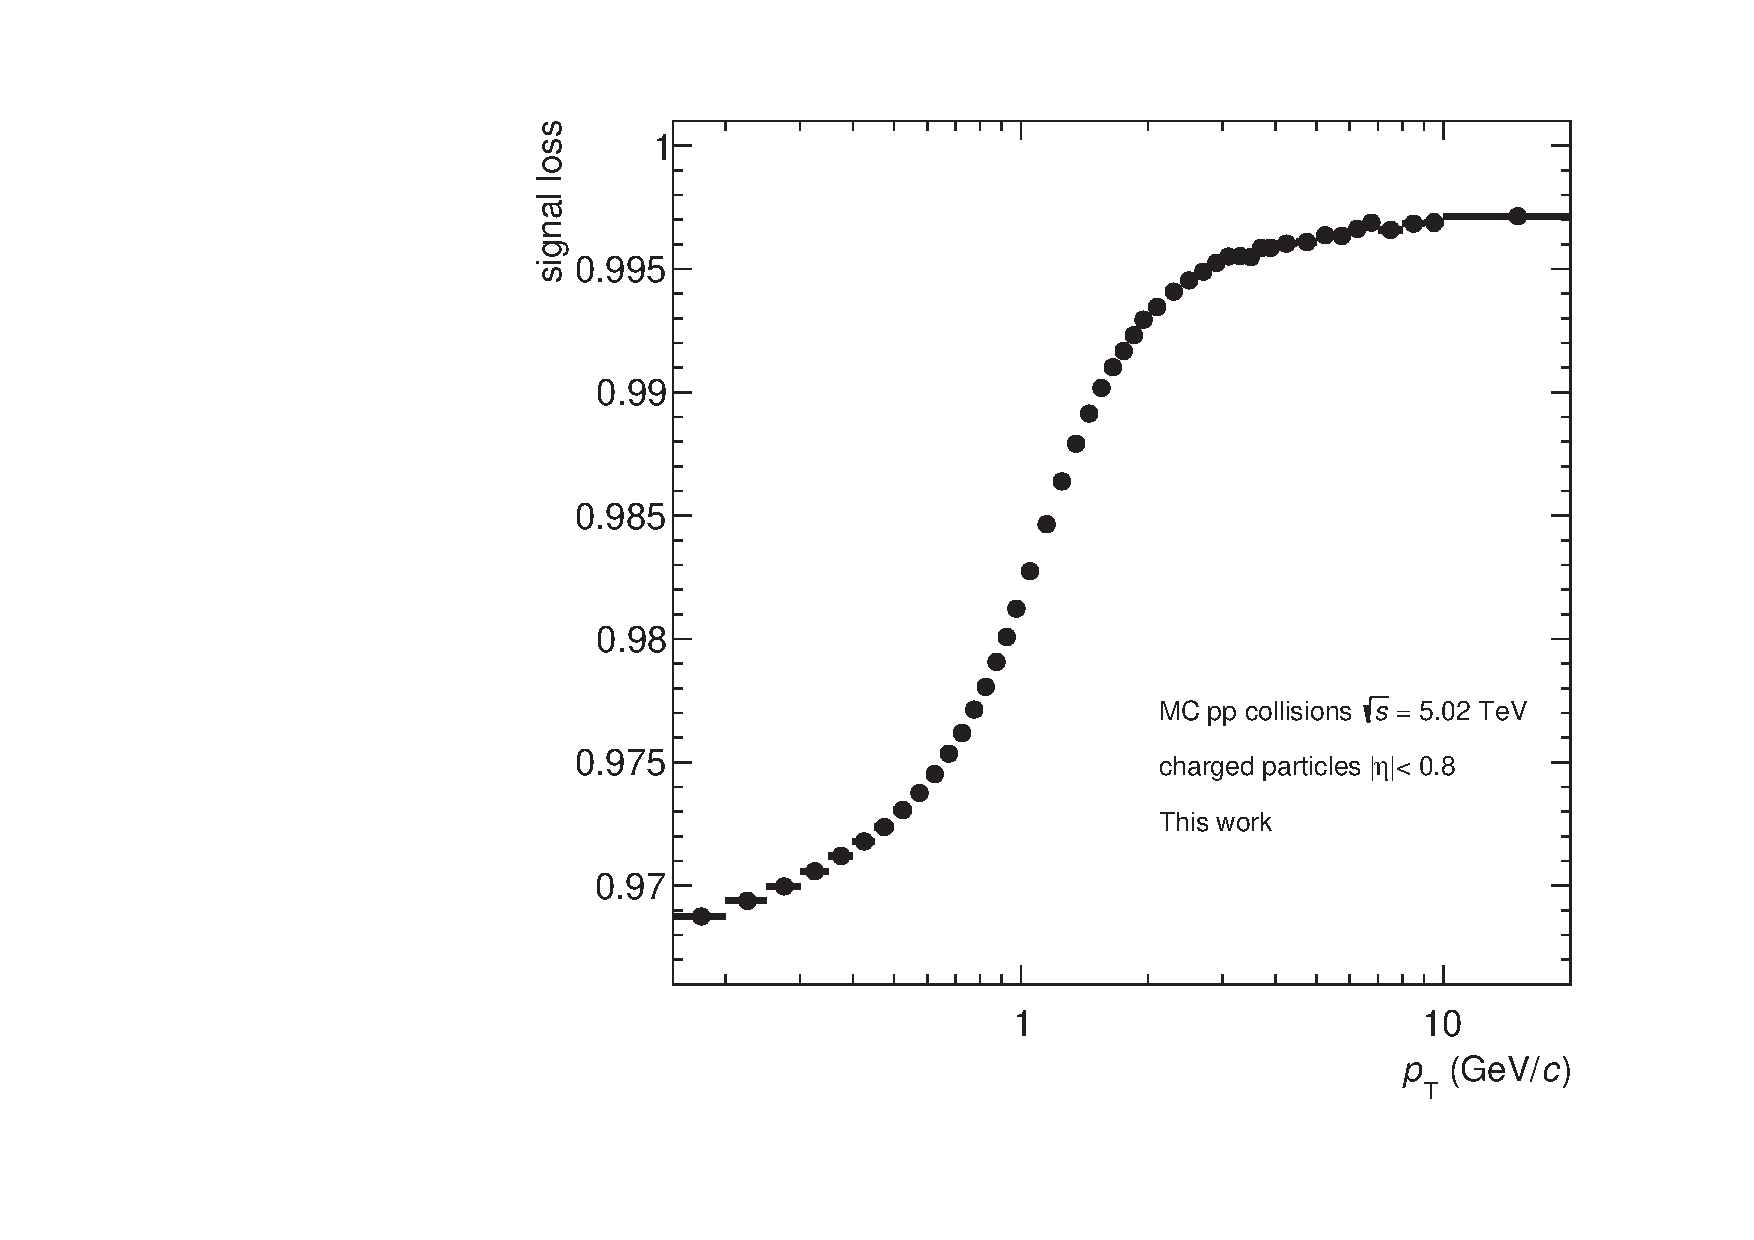
\includegraphics[width=12cm]{Plots/signalLoss.pdf}  
\caption{Signal loss as function of the transverse momentum for pp collisions.}
\label{sigLoss}
\end{figure}
%find reference  
A fraction of the inelastic events is missing due to the trigger and vertex reconstruction efficiency. In order to regain the tracks from missing events, a complementary correction at track-level is required. This is achieved using the MC production to compare the distribution of primary tracks generated from inelastic events within the vertex cut $|V_z| < 10$ cm before and after they undergo the event selection:
\begin{equation}
\chi_\text{s.l.}(p_\text{T}) = \dfrac{(\text{d}N/\text{d}p_\text{T})_\text{Generated}^\text{After event selection}}{(\text{d}N/\text{d}p_\text{T})_\text{Generated}^\text{True INEL, |Vz|<10 cm}}
\end{equation}
As result, the \pt dependent distribution of the signal loss $\chi_\text{s.l.}(p_\text{T})$ is shown in Figure \ref{sigLoss}. The effect is more pronounced at low $p_\text{T}$, where it amounts to about 3\%. The signal loss decreases, becoming negligible above 10 GeV/$c$. The required correction is implemented by scaling the \pt spectrum in each \pt interval with the inverse of the corresponding value of the signal loss.
\subsection{Tracking efficiency and acceptance}
\begin{figure}[tb!]
\centering
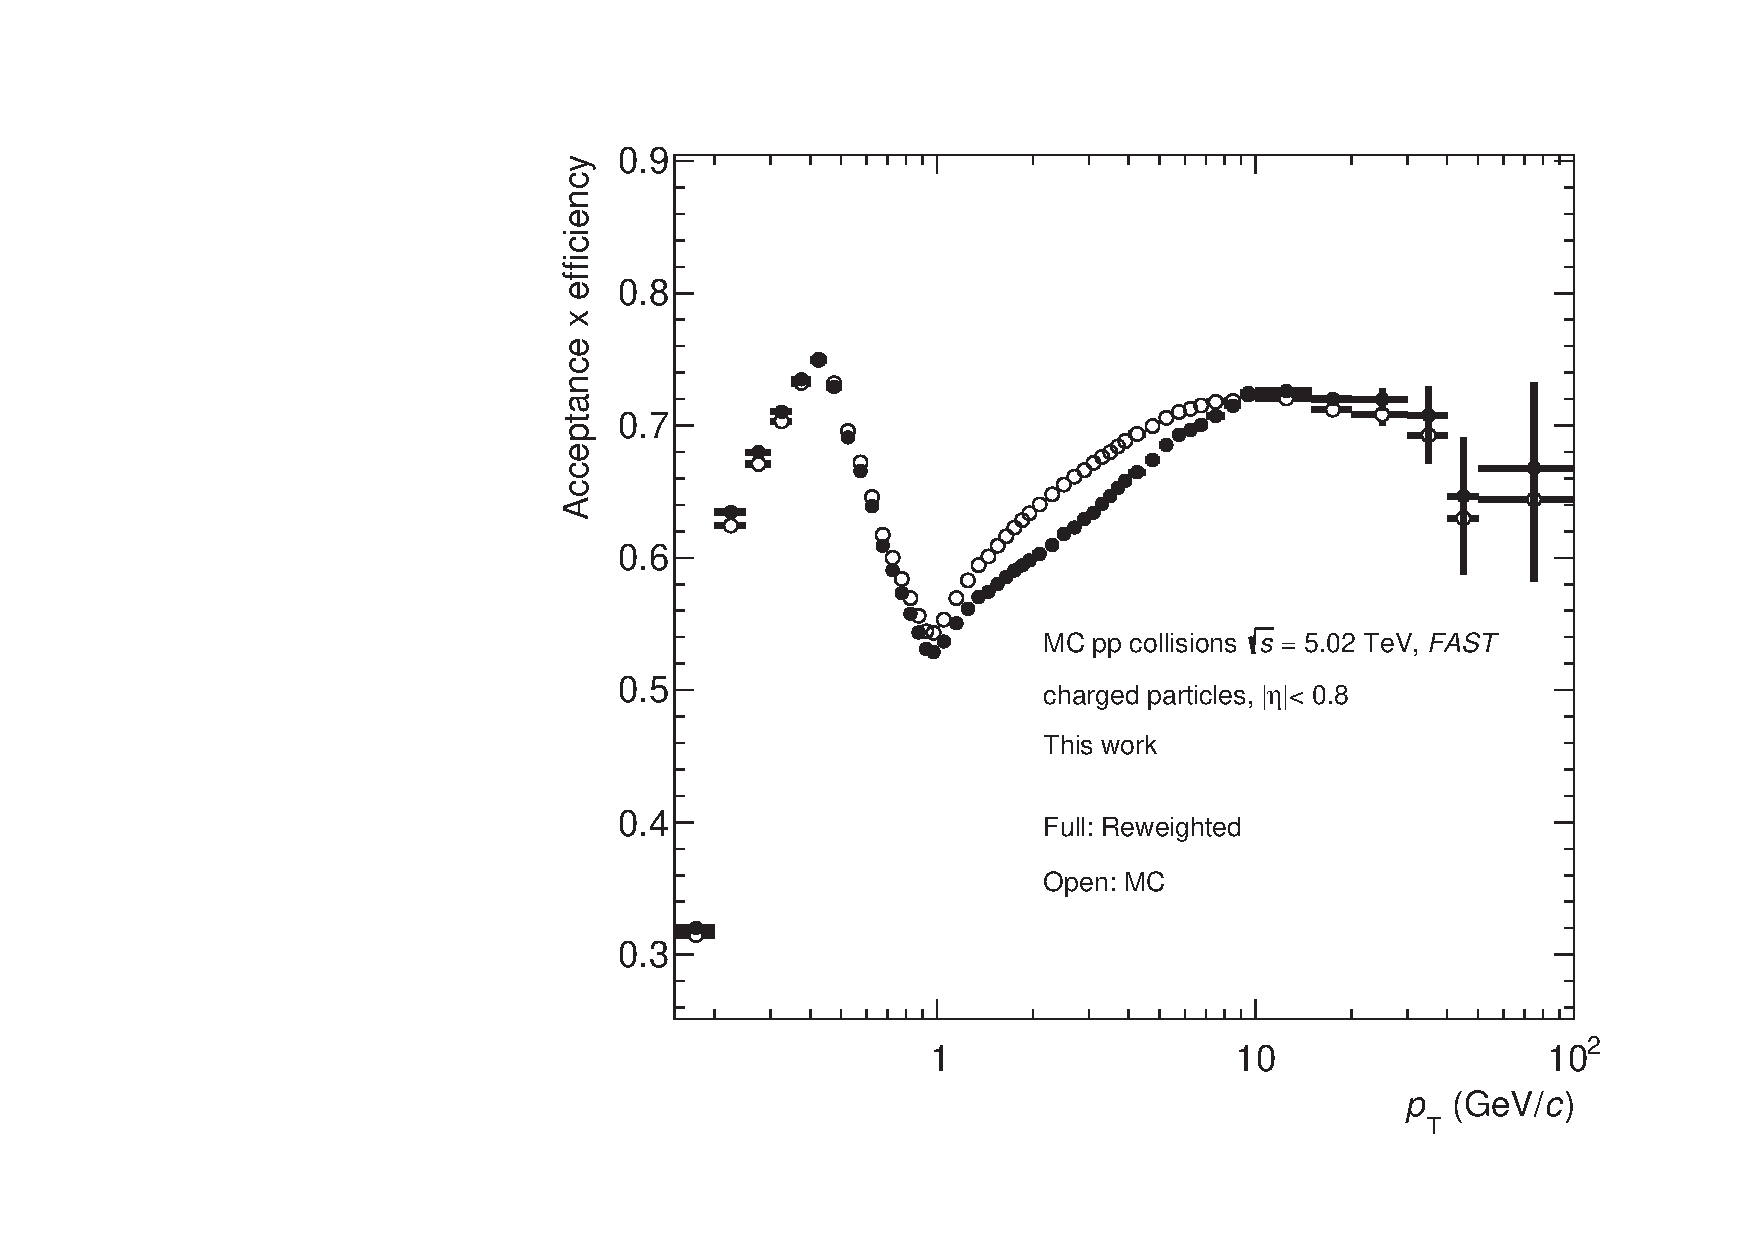
\includegraphics[width=12cm]{Plots/trckEffpp.pdf}  
\caption{Acceptance and tracking efficiency as function of the transverse momentum for pp collisions determined with MC simulations. The overall efficiencies obtained before and after the reweighting are represented with open and full markers, respectively.}
\label{trckEffpp}
\end{figure}
The TPC-ITS detector system is able to measure most of the tracks that cross the detector volume. However, the reconstruction algorithm is sometimes unable to detect a track or to reconstruct it correctly which as consequence results in its discard due to the track selection. Limitations of the geometrical acceptance can affect likewise the track reconstruction and they should be therefore also taken into account. \\
The tracking efficiency and acceptance can be summarized in an overall detection efficiency $\epsilon$ for the reconstruction of tracks which depends on transverse momentum \pt. The implementation of the corresponding correction will thus affect the shape of the \pt distributions. The \pt dependent efficiency is calculated using the MC simulations as the ratio of reconstructed primary charged-particle tracks that survive the track selection $N_\text{prim,rec}^\text{MC}$ to generated primary charged particles $N_\text{prim,gen}^\text{MC}$: 
\begin{equation}
\epsilon(p_\text{T}) = \dfrac{N_\text{prim,rec}^\text{MC}(p_\text{T})}{N_\text{prim,gen}^\text{MC}(p_\text{T})} 
\label{trckEffEq}
\end{equation}
For the correction, the inverse of the overall efficiency is applied as a multiplicative factor in each \pt interval of the \pt spectra.\\
The overall efficiency also depends on the particle type. This requires a complementary correction, explained later on, which scales the overall efficiency by means of the relative abundance of each particle species (cite Patricks thesis).\\
\begin{figure}[tb!]
\centering
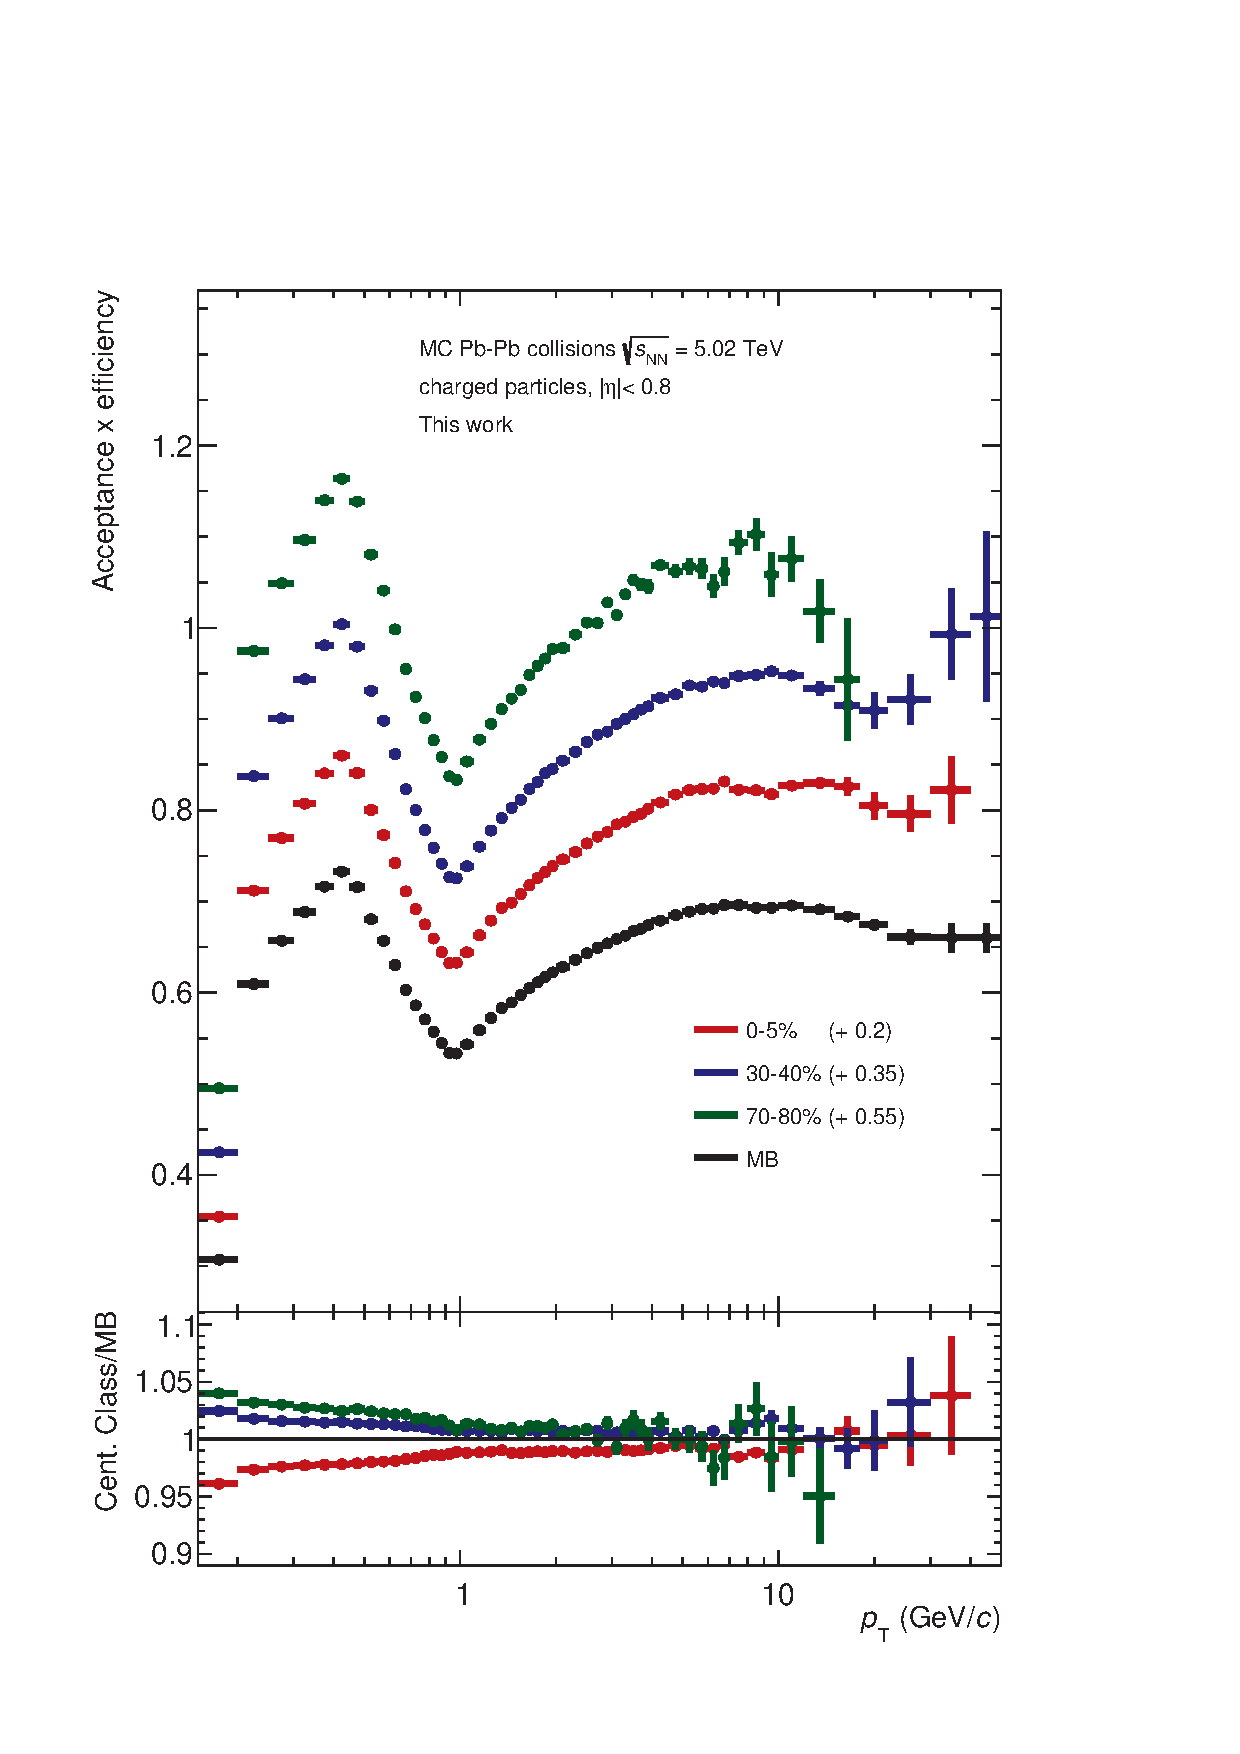
\includegraphics[width=12cm]{Plots/trckEffPbPb1.pdf}  
\caption{Tracking efficiency as function of the transverse momentum for MB, central, semi-central and peripheral Pb-Pb collisions obtained from MC simulations. An offset value is added to the efficiencies for a better visibility. In the bottom panel, the ratio of the individual efficiencies to the MB efficiency is shown.}
\label{trckEffPbPb1}
\end{figure}
\hspace{-0.3cm} In Figure \ref{trckEffpp}, the overall efficiency as function of \pt is shown for pp collisions. Here, the efficiency amounts to a value between 54\% and 75\% over the entire \pt range. At low $p_\text{T}$, below 0.4 GeV/$c$, there is a rapid growth of the efficiency which can be explained by the increasing radii of the particle trajectories making it more likely for the track to fulfil the strict selection criteria. After reaching the maximum, the curve drops quickly and hits its minimum around 1 GeV/$c$. This slump is caused mainly by the track length cut listed in Table \ref{tab:Cuts} which aims for a selection of tracks that fulfil a minimal geometric length within the fiducial detector volume. The tracks in the $p_\text{T}$-range of the slump tend to cross the TPC boundaries so that they are less likely to be selected. Following this, the distribution increases asymptotically due to the acceptance restrictions of the detector up to reaching a plateau (cite paper). At even higher $p_\text{T}$, the trend hint at a declining efficiency. Nevertheless, the overall efficiency is assumed to be constant for $p_\text{T} \geq 40$ GeV/$c$ in order to reduce statistical fluctuations. 
\begin{table}[tb!]
\centering
\renewcommand{\arraystretch}{1.5}
\begin{tabular}{|c|c|}
\toprule
\rowcolor{headerBlue} \textbf{Centrality class} &  \textbf{Scaling factor}\\
\midrule
0-5\%	&	0.980	 \\
5-10\%	&	0.989	 \\
10-20\%	&	1.000	 \\
20-30\%	&	1.010	 \\
30-40\%	&	1.014	 \\
40-50\%	&	1.018	 \\
50-60\%	&	1.021	 \\
60-70\%	&	1.023	 \\
70-80\%	&	1.024	 \\
\bottomrule
\end{tabular}
\caption{Scaling factors obtained from the parametrization of the ratios in Figure \ref{trckEffPbPb1}.}
\label{tab:ScalingFactors}
\end{table}
\begin{figure}[tb!]
\centering
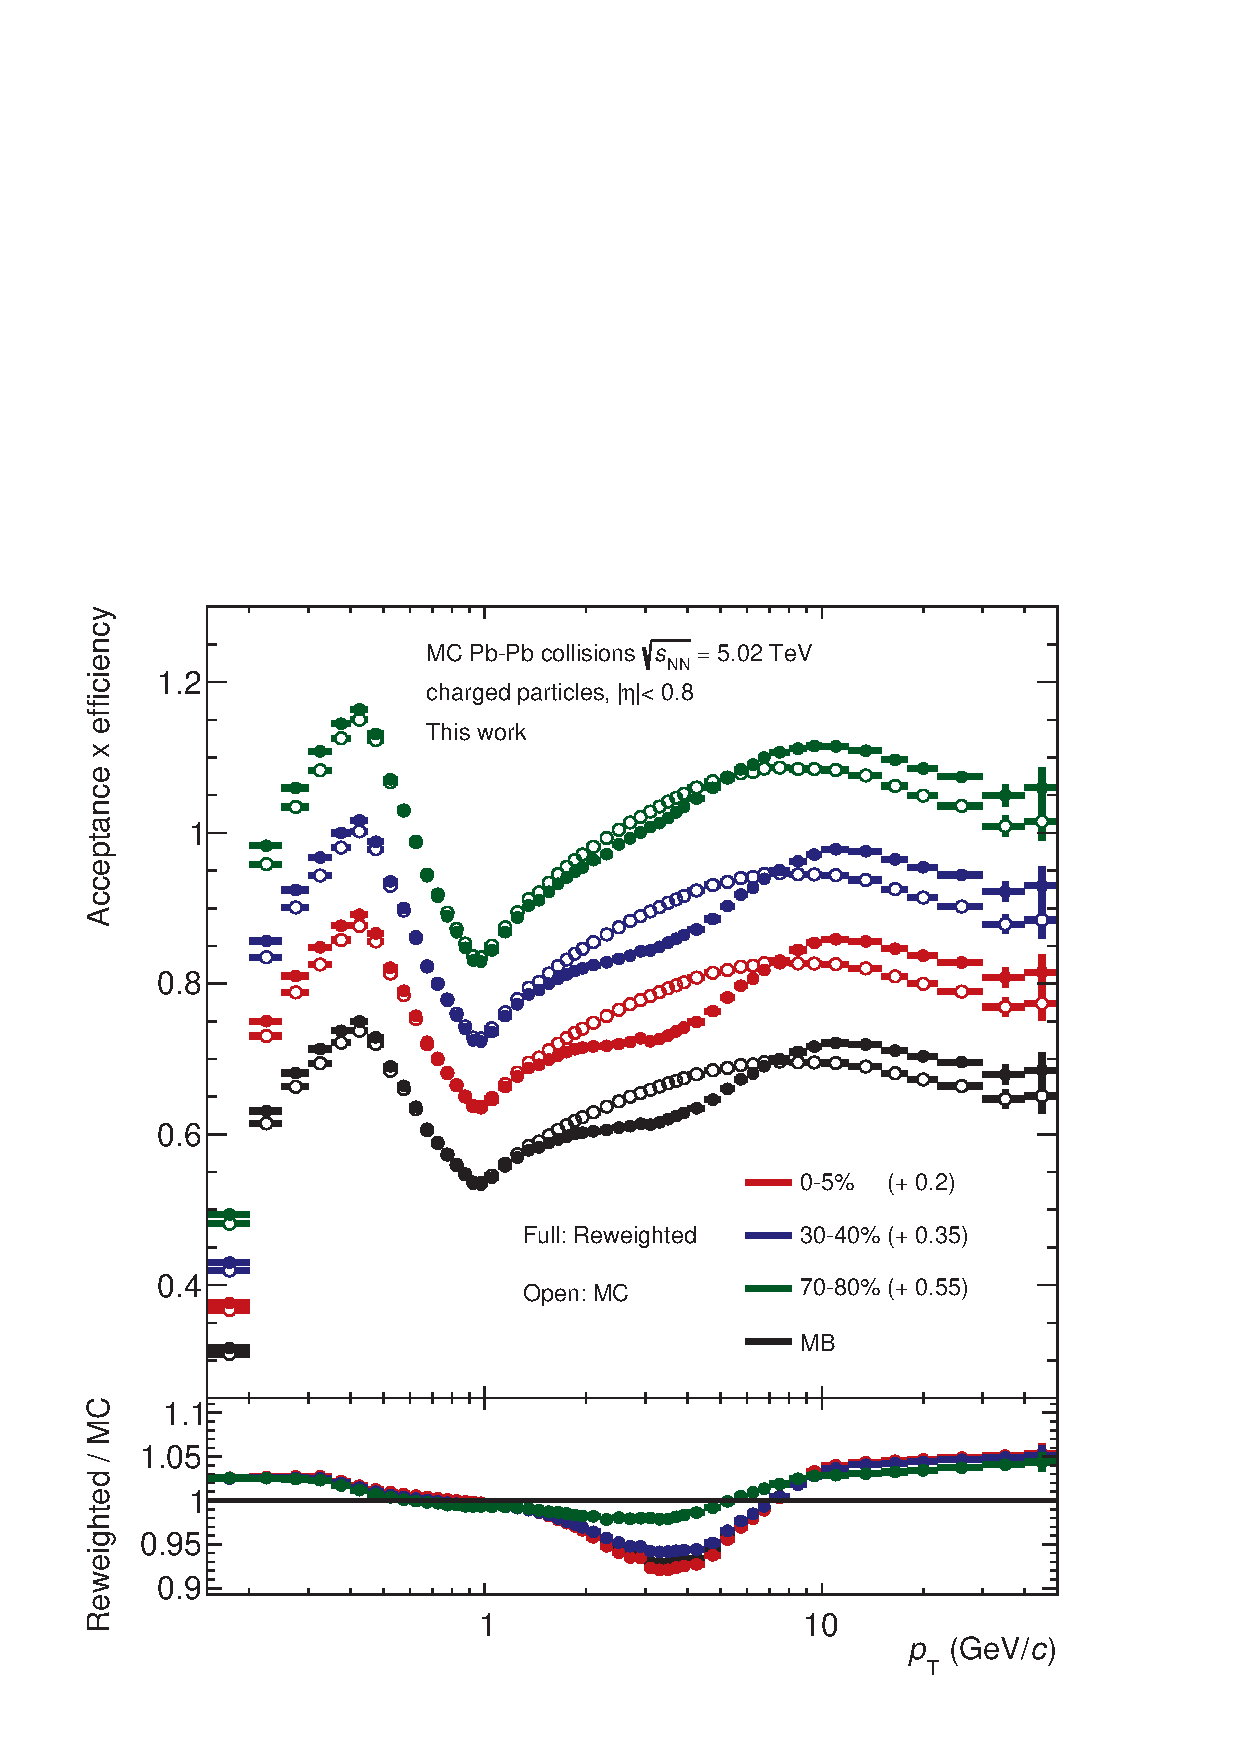
\includegraphics[width=12cm]{Plots/trckEffPbPb2.pdf}  
\caption{Tracking efficiency as function of the transverse momentum for MB, central, semi-central and peripheral Pb-Pb collisions obtained from the scaling of the distributions in Figure \ref{trckEffPbPb1} using the values listed in Table \ref{tab:ScalingFactors}. The overall efficiencies obtained before and after the reweighting are represented with open and full markers, respectively. An offset value is added to the efficiencies for a better visibility.}
\label{trckEffPbPb2}
\end{figure}
\hspace{-0.3cm} This same trend of the efficiency is also observed for the Pb-Pb collisions analysed in this thesis as illustrated in Figure \ref{trckEffPbPb1}, which shows the efficiency as function of \pt for MB, central ($0-5$\%), semi-central ($30-40$\%) and peripheral ($70-80$\%) collisions. Here, it is observed that the efficiency decreases with centrality. Towards peripheral collisions, the high \pt range of the centrality-dependent efficiencies is dominated by increasing statistical fluctuations. To avoid the propagation of these fluctuations to the corrected \pt spectra, the ratios of the individual efficiencies to the MB efficiency, illustrated in the bottom panel, are parametrized in the range 1.5 GeV/$c$ < \pt < 10 GeV/$c$ with a constant function. The obtained factors, summarized in Table \ref{tab:ScalingFactors}, are used to scale the MB tracking efficiency for \pt > 1.5 GeV/$c$, while the original efficiencies are used below this range. As result, the distributions obtained using this approach are represented in Figure \ref{trckEffPbPb2} with open markers. 
\subsubsection{Particle composition correction}
%https://pdg.lbl.gov/2020/citation.html
\begin{figure}[tb!]
\centering
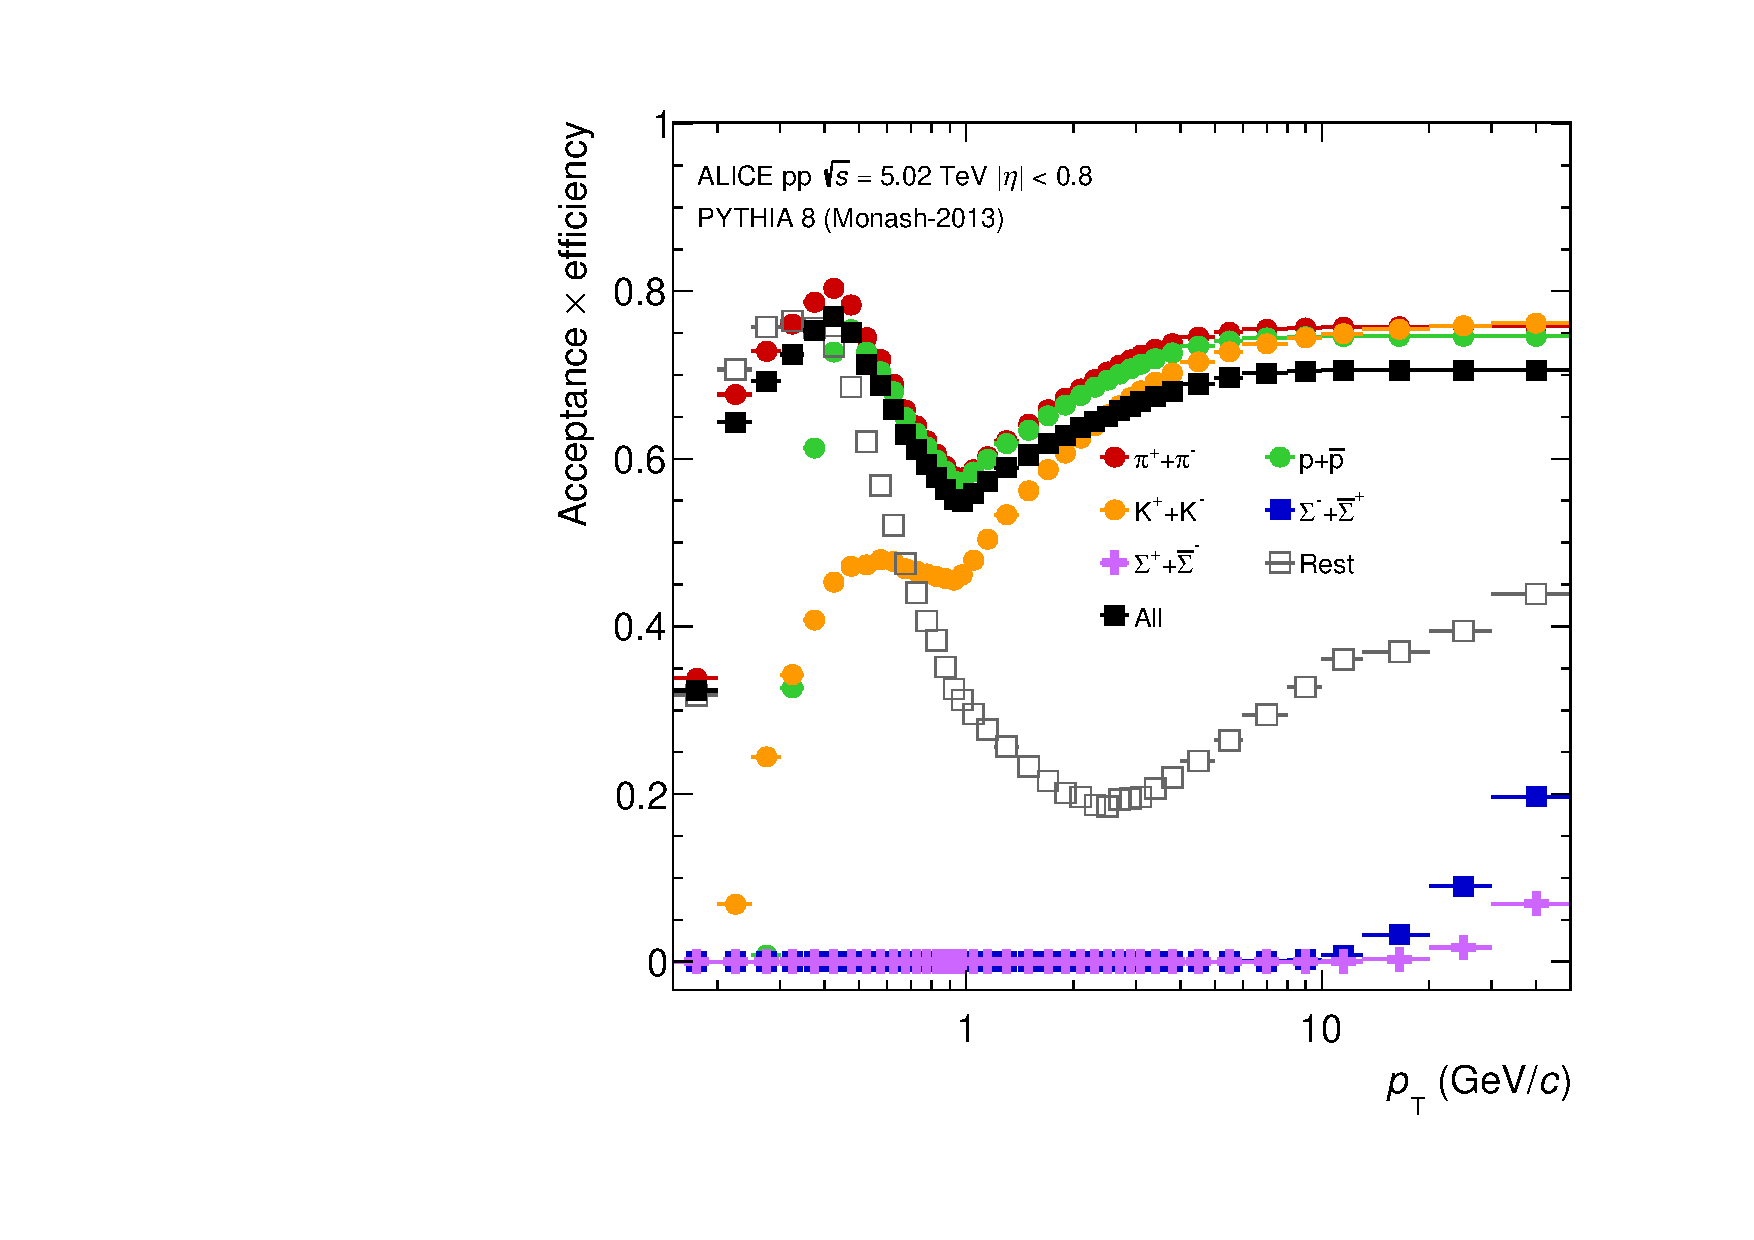
\includegraphics[width=0.495\textwidth]{Plots/5TeVMonash13_TrkEff_without-91972.pdf}  
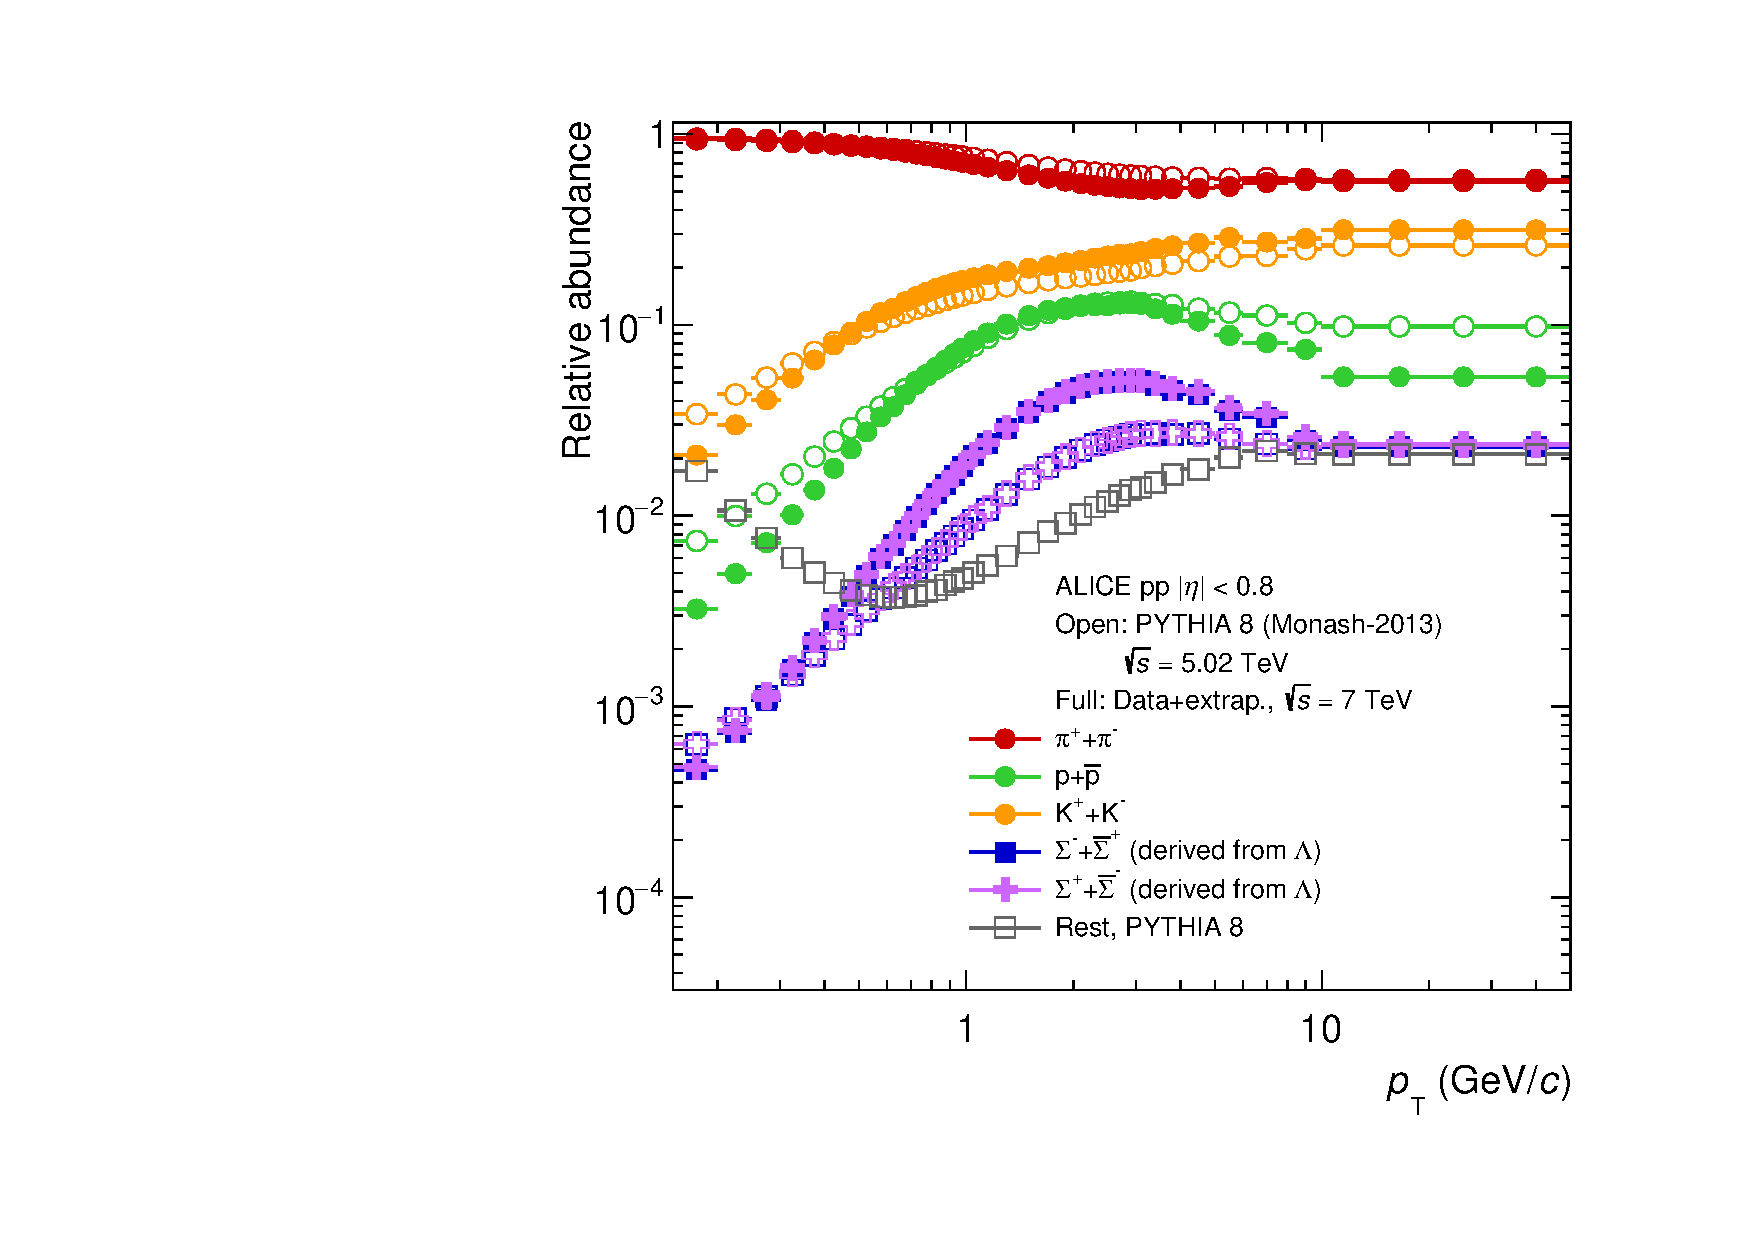
\includegraphics[width=0.495\textwidth]{Plots/5TeVMonash13_Abundances-91973.pdf}  
\caption{\textbf{Left: }Tracking efficiencies as function of the transverse momentum for different particle species obtained with a PYTHIA (Monash 13) simulation of pp collisions at $\sqrt{s} = 5.02$ TeV. \textbf{Right:} Relative particle abundances as function of the transverse momentum in data (full symbols,  $\sqrt{s} = 7$ TeV) and in MC (open symbols,  $\sqrt{s} = 5.02$ TeV) (cite paper).}
\label{trckEffParticles}
\end{figure}
Primary charged particles present a wide disparity in terms of lifetime. For instance, the pions ($\pi^{\pm}$), the most frequent particle type produced in particle collisions, can travel on average $7.8\text{ m}$ within their lifetime, whereas the sigma baryons ($\Sigma^{\pm}$) have a decay length of only $2.4\text{ cm}$ (cite pdg booklet). As consequence, some particles are more likely to be rejected by the track length requirement than others, which results in the tracking efficiency depending on the particle type. \\
The use of MC event generators, such as PYTHIA or HIJING, allows to obtain the tracking efficiencies for different particle species as shown in the left panel of Figure \ref{trckEffParticles}. Here, results from  an analysis of the particle dependent efficiency for pp collisions at $\sqrt{s} = 5.02$ TeV are presented (cite paper). As shown in the Figure, the dependence of the efficiency on the particle type is strong, especially below $1$ GeV/$c$. In Pb-Pb collisions, similar effects are observed as can be seen in Appendix \ref{TrkEffApp}. Because of these similarities, the correction procedure is only shown for pp collisions, although an analogous procedure is also implemented for Pb-Pb collisions.\\
Considering the particle type dependence of the efficiency, the abundance of each particle plays an important role for the particle type inclusive efficiency and must therefore be reflected in the correction. However, MC event generators can not entirely reproduce the production of strange particles (cite 38,39 paper). As consequence, the efficiency is considerably affected by an underestimation of this production and a correction by means of a reweighting of the efficiency with the relative abundance of each particle type is implemented. The right plot of Figure \ref{trckEffParticles} shows the relative abundances measured in pp collisions recorded by ALICE at $\sqrt{s} = 7$ TeV. This centre-of-mass energy is used since no significant energy dependence has been observed experimentally and because of the lack of experimental data at the energy studied in this work (cite Patrick). The relative abundances used in this thesis were calculated by the cited analysis using a data-driven procedure and correspond to the same distributions used in the previous ALICE measurement of nuclear modification factors (cite paper).\\
In summary, the tracking efficiency for inclusive particles should be understood as a weighted superposition of the individual efficiencies for each particle type with the relative particle abundances. Based on this, a \pt dependent correction for the efficiencies was determined in this analysis (cite Patrick). After applying the reweighting on the distributions represented in Figures \ref{trckEffpp} and \ref{trckEffPbPb2} with open symbols, the corrected tracking efficiencies for inclusive charged particles are obtained and shown with full markers. In the bottom panel, the ratio of the reweighted efficiency to the efficiency from pure MC is shown. This reflects the effect of the particle composition correction. The reweighted efficiencies are utilized ultimately to correct the \pt distributions. 
\subsection{Contamination by secondary particles}
The selection procedure described in Section \ref{TrackSelection} aims to reduce the contamination of the measured track sample with secondary particles. Nevertheless, a small amount of these particles persists in it. This remnant originates from weak decays of kaons, $\Lambda$ baryons and muons as well as from interactions with the detector material. The remaining fraction of secondary particles has to be subtracted from the raw \pt distributions to ensure the purity of the data.\\
The contamination by secondaries is estimated using the MC productions anchored to the analysed data periods. In Figure \ref{SecCont}, the secondary contamination from pure MC is shown with open markers for pp collisions as well as for central ($0-5$\%), semi-central ($30-40$\%) and peripheral ($70-80$\%) Pb-Pb collisions. In general, the contamination reaches a percentage value of around  $10\%$ in the first \pt interval. The distributions then fall monotonously with increasing \pt below $1\%$ in the high \pt region. These observations are consistent with the assumption that secondaries are inclined to carry small momenta since they correspond essentially to fractions of the momenta of the mother particles or are created in interactions with the detector material. In Pb-Pb collisions, the contamination depends on the centrality. At low $p_\text{T}$, the contamination in central collisions ($0-5$\%) amounts to almost twice as much as the contamination in the most peripheral ($70-80$\%) collisions. This is a result of an enhancement of the yield of strange particles observed in systems with high energy densities (cite here). The centrality dependence becomes less pronounced in the high $p_\text{T}$ range.
\begin{figure}[tb!]
\centering
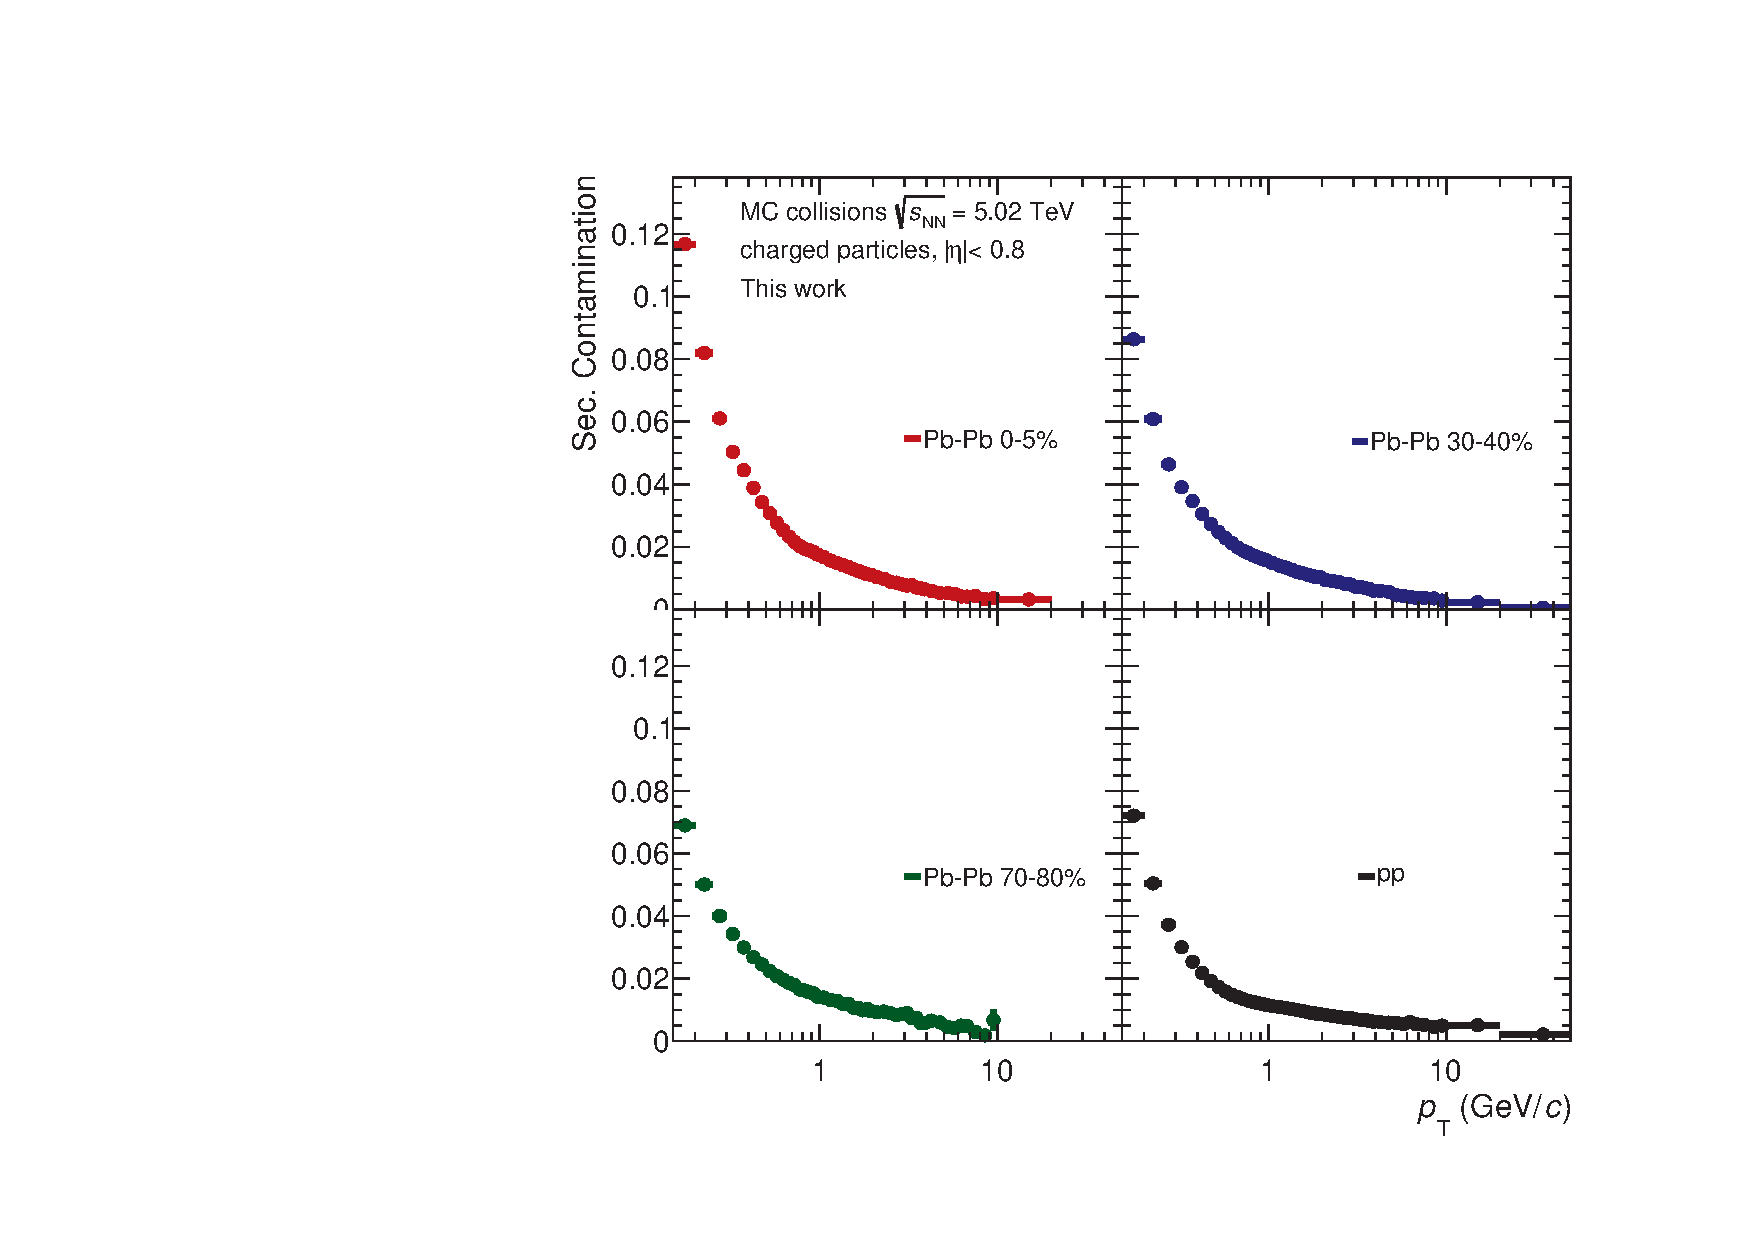
\includegraphics[width=12cm]{Plots/secCont.pdf}  
\caption{Contamination with secondary particles as function of the transverse momentum obtained from MC simulations for pp collisions as well as central, semi-central and peripheral Pb-Pb collisions. Open markers represent the secondary contamination obtained from pure MC, while the full ones correspond to the  corrected contamination.}
\label{SecCont}
\end{figure}
\subsubsection{Secondary scaling}
%cite TFractionFitter A la HMCMLL, see R. Barlow and C. Beeston, Comp. Phys. Comm. 77 (1993) 219-228, and http://www.hep.man.ac.uk/~roger/hfrac.f
\begin{figure}[tb!]
\centering
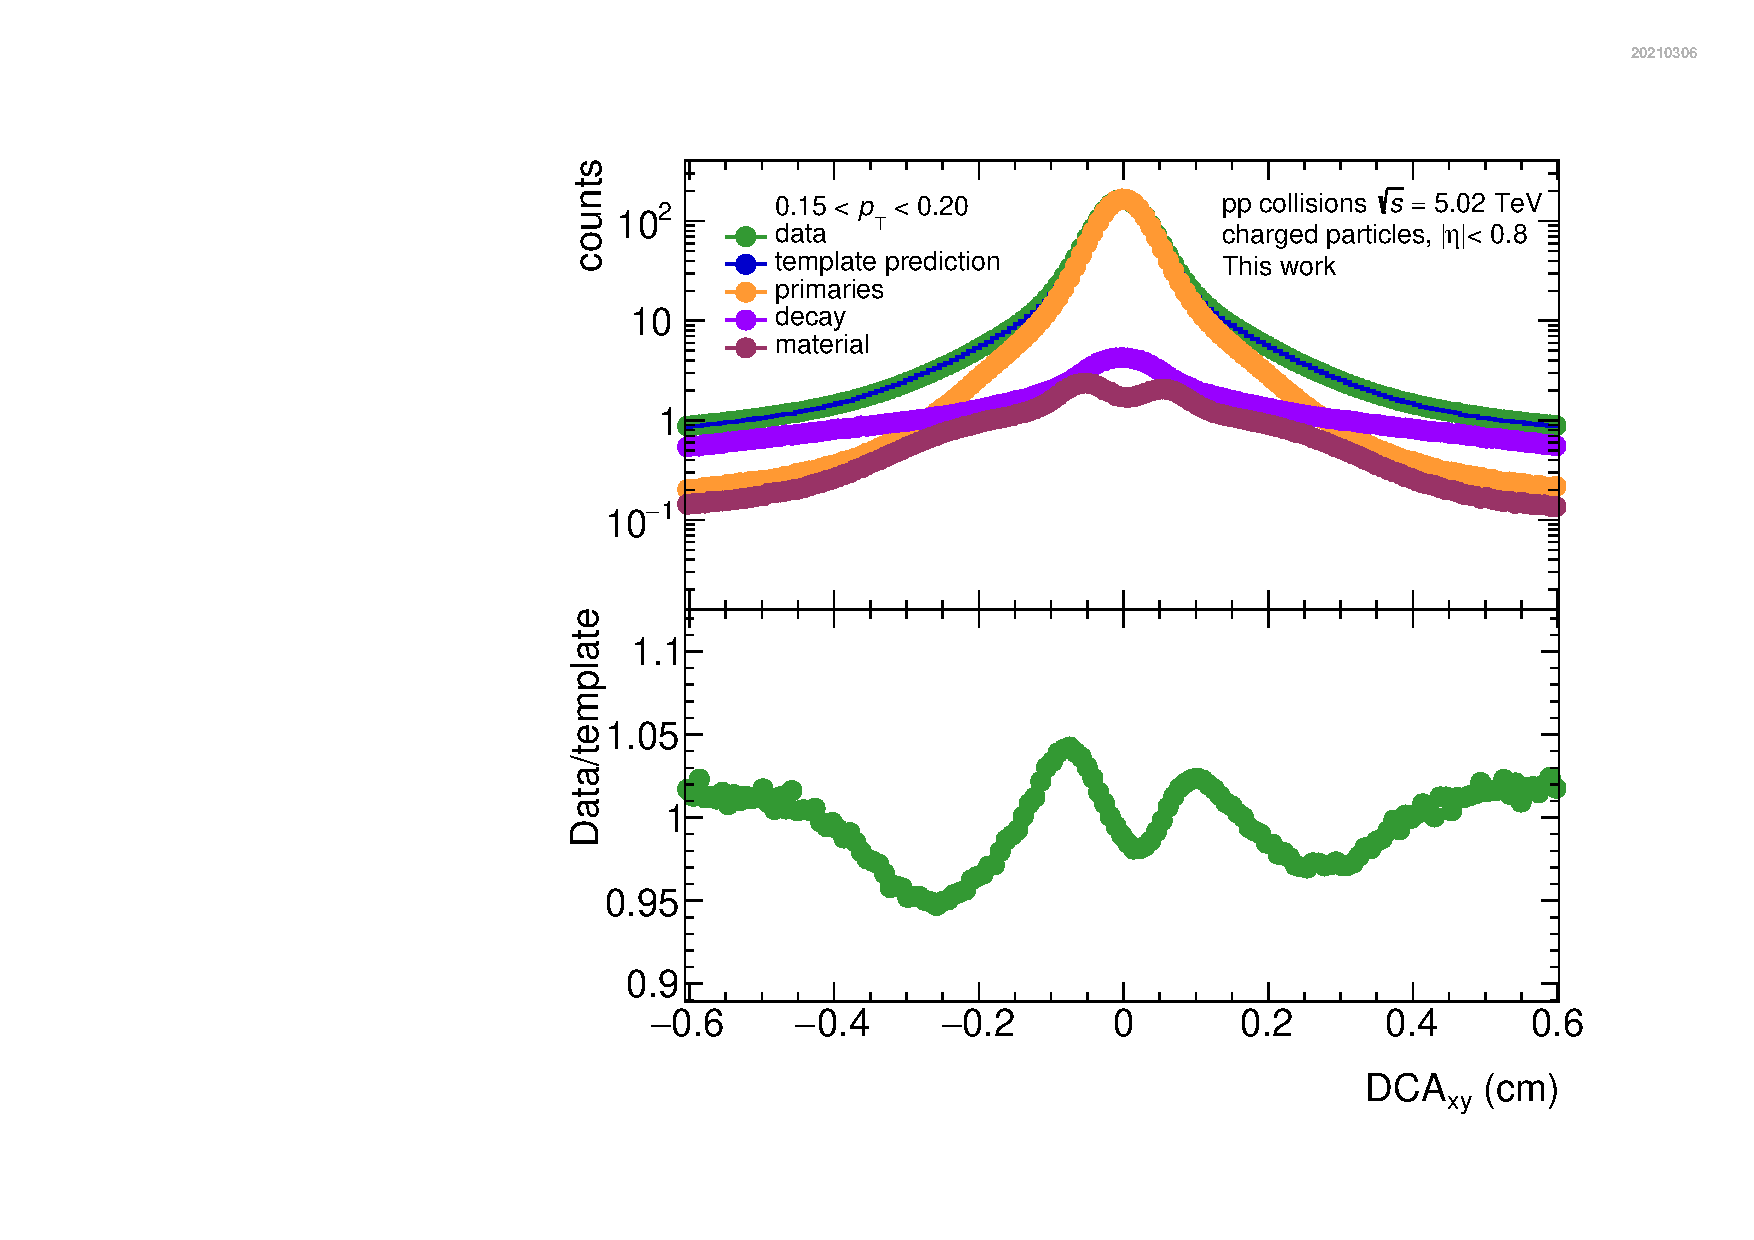
\includegraphics[width=12cm]{Plots/DCAdistributions.pdf}  
\caption{DCA$_\text{xy}$ distributions for data and MC simulations for pp collisions at $\sqrt{s} = 5.02$ TeV for the \pt range $0.15 \leq $ \pt $< 0.19$ GeV/$c$. The MC predictions correspond to primaries, secondaries from decay and secondaries from interactions in the detector material. In the bottom panel, the ratio of distribution for data to the fit resulting from the MC templates is shown.}
\label{secScaling}
\end{figure}
As stated in the previous section, MC productions underestimate the yield of strange particles. Since the decay products of strange particles are highly prevalent among secondaries, the distributions shown in Figures \ref{SecCont} do not reflect entirely the true secondary contamination. To correct for this effect, first the relative abundance of secondaries in data $\rho_\text{Data}$ is determined in each \pt interval using the approach explained below. Then, a scaling factor is calculated as:
\begin{equation}
c_\text{sec. sca.} = \dfrac{\rho_\text{Data}}{\rho_\text{MC}}
\end{equation}
where $\rho_\text{MC}$ represents the fraction of secondaries in the MC sample. The secondary contamination from pure MC is then reweighted in each \pt interval with the corresponding scaling factor.\\
The distance of closest approach (DCA) is used as baseline to discriminate between primaries and secondaries in the data sample. By that, the required fraction $\rho_\text{Data}$ can be determined. Since secondaries are originated at a later stage than primaries, the respective DCA$_{\text{xy}}$ distributions present distinct shapes. The differences should arise particularly in the region of the tails, where the largest DCA$_{\text{xy}}$ values are located. In this regard, the track selection must be modified in order to obtain a statistically significant result. In particular, the new track selection dispenses with the cuts on the DCA$_\text{xy}$ and on the  $\chi^2_\text{TPC-ITS}$, both of which suppress the yield of secondaries. This modification of the track selection allows to measure an amount of secondaries sufficiently large to extract scaling factors for a few intervals at low $p_\text{T}$ in the range $0.15 \leq p_\text{T} < 1.5 $ GeV/$c$.\\
In the upper panel of Figure \ref{secScaling}, the DCA$_{\text{xy}}$ distribution for pp collisions recorded by ALICE is illustrated for the \pt interval $0.15 \leq p_\text{T} < 0.2 $ GeV/$c$. In the same figure, the corresponding MC predictions of the DCA$_{\text{xy}}$ in pp collisions for primaries, secondaries from decays and secondaries originating from interactions in the detector material are represented. Primaries present a shape with a prominent peak at $0$ cm that far exceeds the small peaks that characterize both distributions of secondaries. Differences are also noticeable towards larger DCA$_{\text{xy}}$, where secondaries, as expected, exhibit much broader tails. The data distribution clearly resembles the shape for primary particles since these dominate the particle production. These observations also apply for all $p_\text{T}$ intervals and also for the case of Pb-Pb collisions as it can be seen in the corresponding figures in the Appendix (cite here). \\
Next, the DCA$_{\text{xy}}$ distribution in data is fitted with a linear combination of the MC templates (cite TFractionFitter). This method takes into consideration statistical uncertainties both from data and MC for a more accurate template fit. The resulting template fit provides as result the wanted fraction $\rho_\text{Data}$, which allows for the calculation of the scaling factor $c_\text{sec. sca.}$.The lower panel of Figure \ref{secScaling} shows the ratio of the distribution for data to the result of the template fit. \\
The intervals of the DCA$_{\text{xy}}$ distributions as well as the \pt intervals for which the fit is performed are adjusted by minimizing the deviation of the data points from the fit as function of the DCA$_{\text{xy}}$ as shown in Figure \ref{Pulls}. Here, it can be seen that the template fit is in good agreement with the data points in the tails, the region of interest in this approach.\\
To ensure the goodness of the fit, a Pearson's chi-squared test was performed with a significance level of $0.05$ (cite Karl Pearson paper). In this approach, the test statistic ratio $\chi^2$ is computed as follows:
\begin{equation}
\chi^2 = \sum_{\text{i}} \dfrac{(\text{DCA}_\text{data,i} - \text{DCA}_\text{fit,i})^2}{\text{DCA}_\text{fit,i}}
\end{equation}
Following this, the critical $\chi^2$ value is calculated by means of the chi-squared probability distribution function determined by the the number of degrees of freedom in the fit and the significance level. According to the chi-squared test, the evaluated fit is rejected whenever the test statistic $\chi^2$ exceeds the critical $\chi^2$ value. All fits used for the calculation of the scaling factors are statistically significant according to this test. \\
\begin{figure}[tb!]
\centering
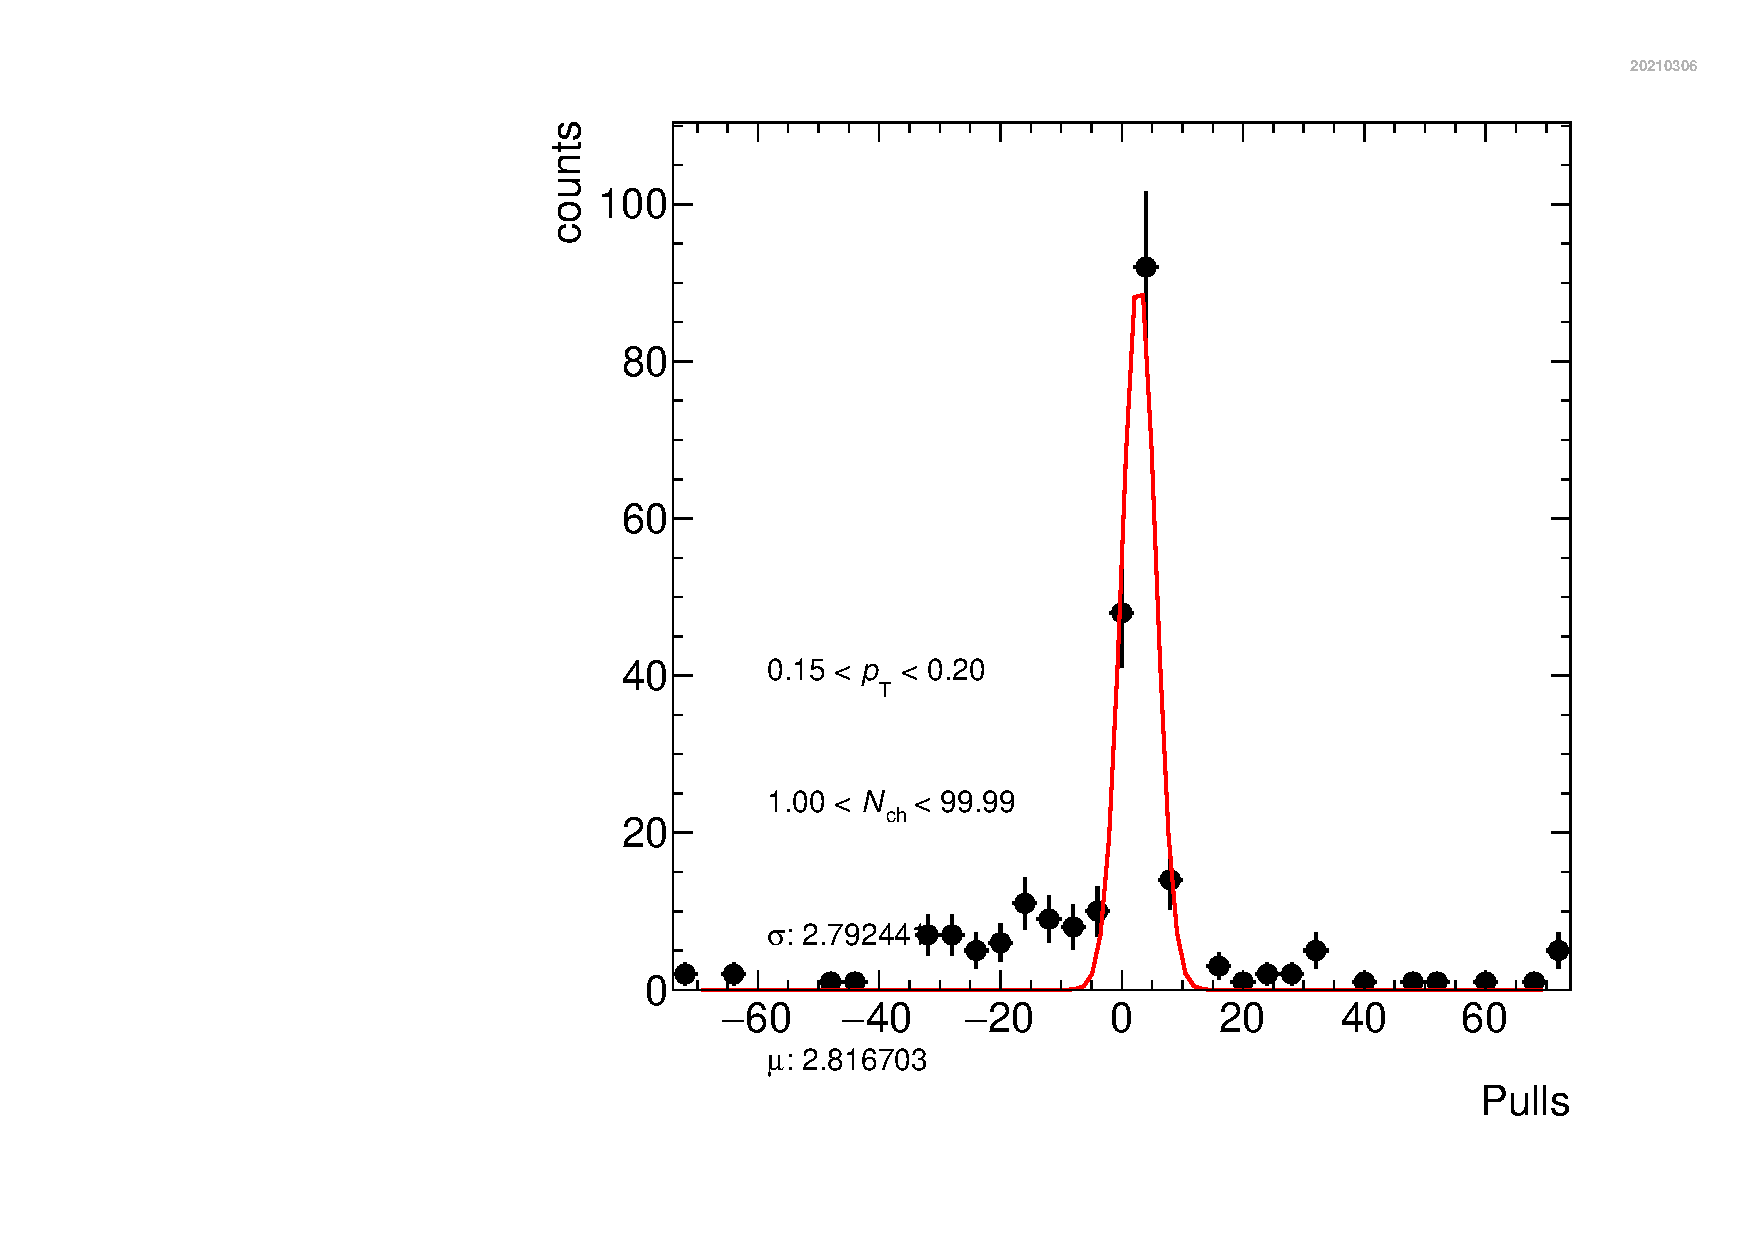
\includegraphics[width=11cm]{Plots/Pulls_Pt0_Mult0.pdf}  
\caption{Deviation of the template fit from the data points as function of the DCA in pp collisions for the \pt interval $0.15 \leq$ \pt $0.19$ GeV/$c$.}
\label{Pulls}
\end{figure}
\hspace{-0.6cm} In Figure \ref{scalefactors}, the resulting scaling factors in pp collisions are shown in the considered \pt intervals with red open markers. In Pb-Pb collisions, the same approach is used. Given that the \pt spectra are represented with a much finer granularity in \pt, the scaling factors are reconstructed through a linear interpolation as shown in this same figure with blue full markers. For \pt $> 1.5$ GeV/$c$, the scaling factor of the last \pt interval is used since the amount of secondaries barely varies beyond this range. The corrected contaminations by secondaries are shown in Figure \ref{SecCont} with full markers.
\begin{figure}[tb!]
\centering
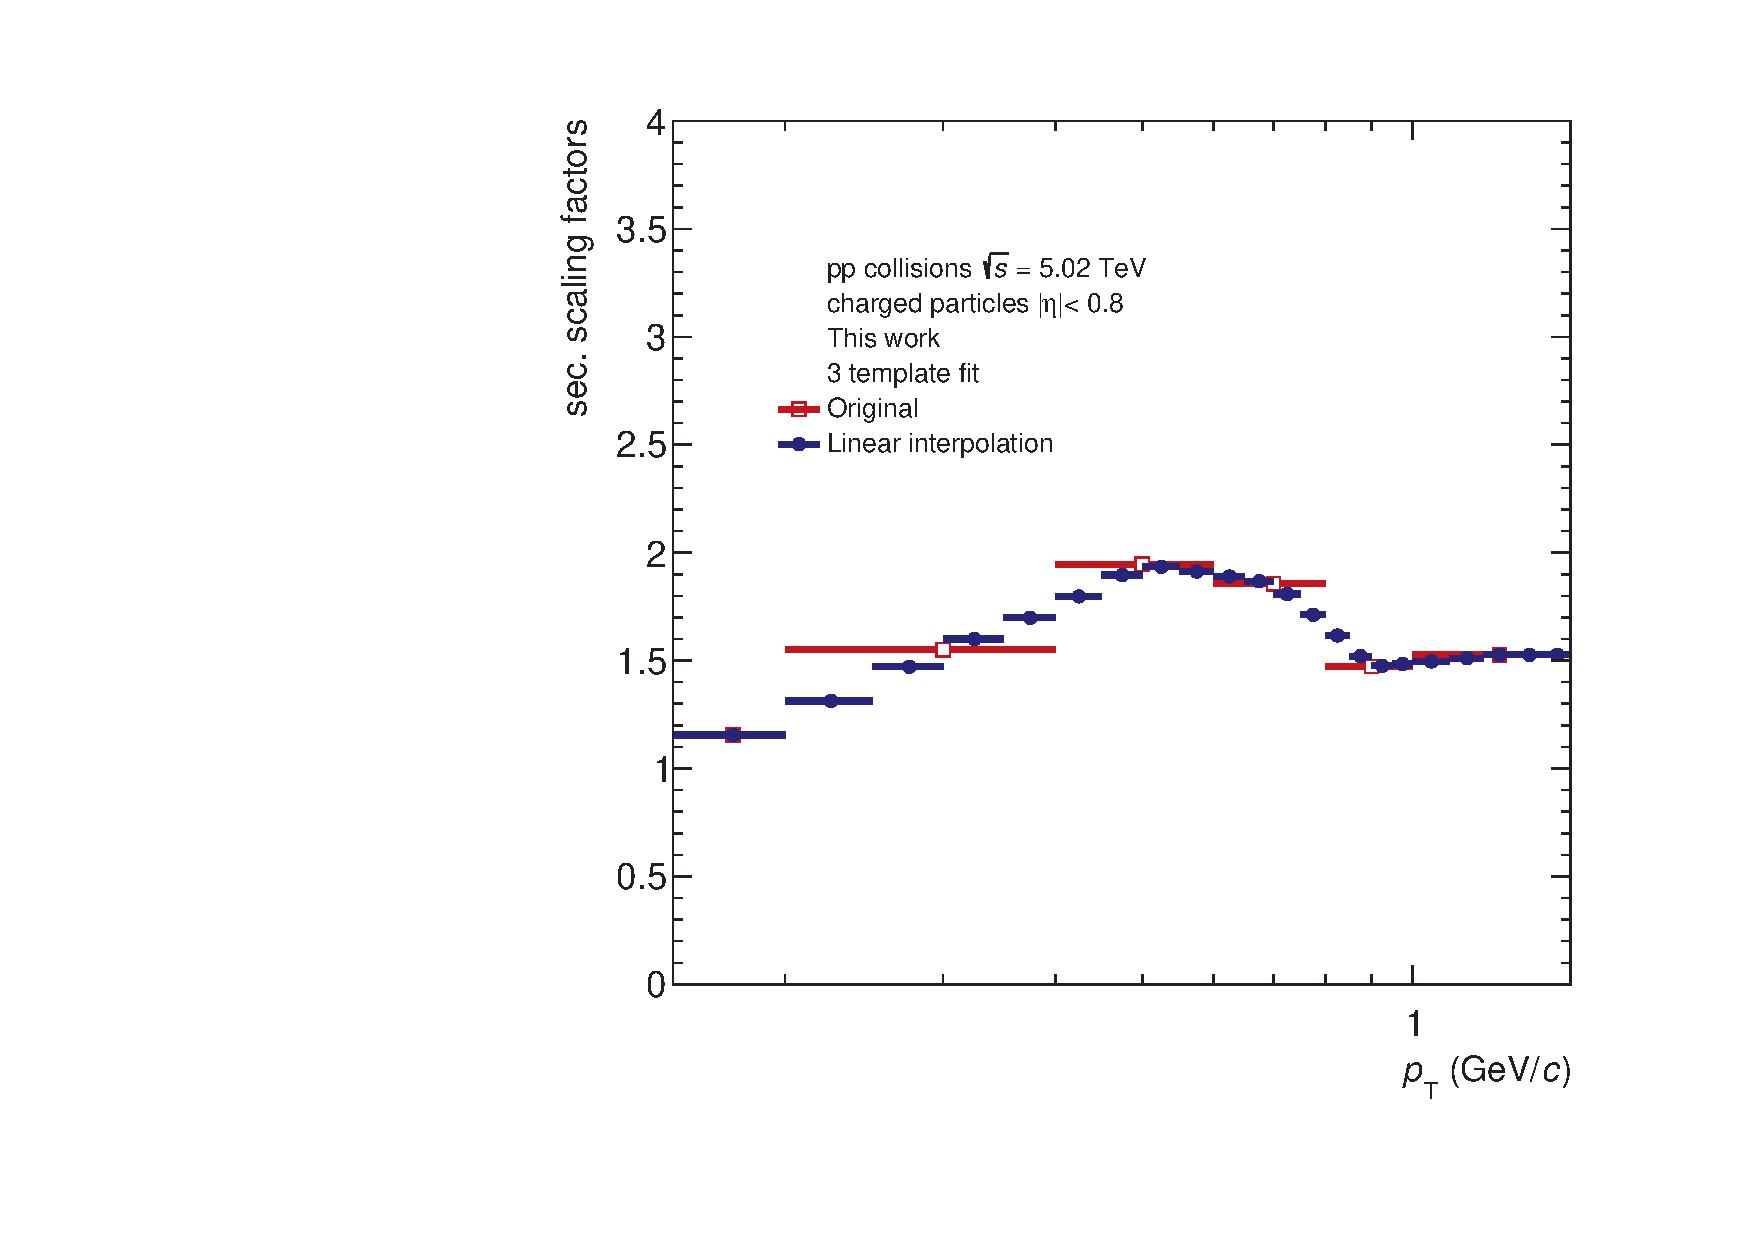
\includegraphics[width=11cm]{Plots/secscalingfactors.pdf}  
\caption{Scaling factors used in pp collisions for the correction of the secondary contamination before and after a linear interpolation.}
\label{scalefactors} 
\end{figure}
\subsection{Transverse momentum resolution}
%cite https://www.physi.uni-heidelberg.de/~fschney/detektoren/detector6.pdf
\begin{figure}[tb!]
\centering
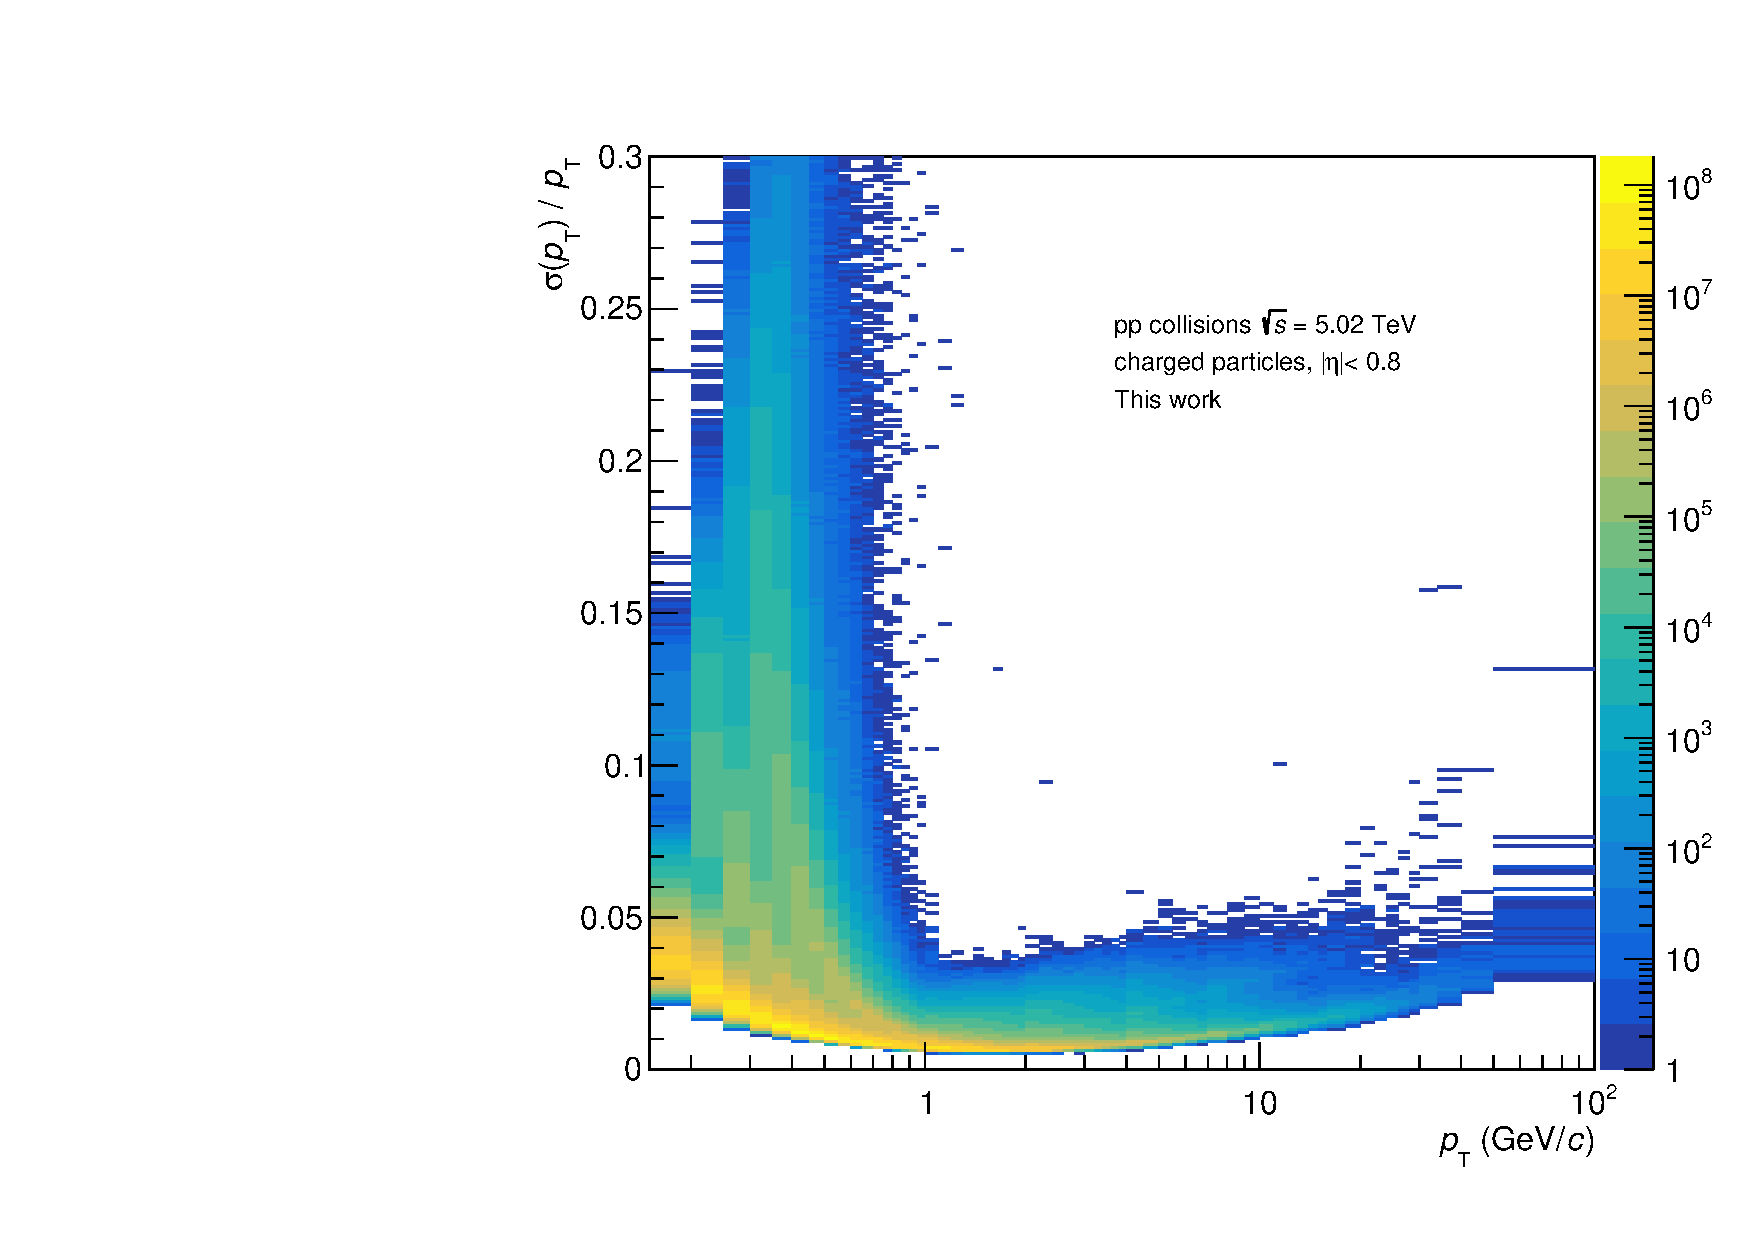
\includegraphics[width=12cm]{Plots/ptReso2D.pdf}  
\caption{Transverse momentum resolution as function of the transverse momentum for pp collisions at $\sqrt{s} = 5.02$ TeV recorded in ALICE in 2017.}
\label{ptReso2D}
\end{figure}
\begin{figure}[tb!]
\centering
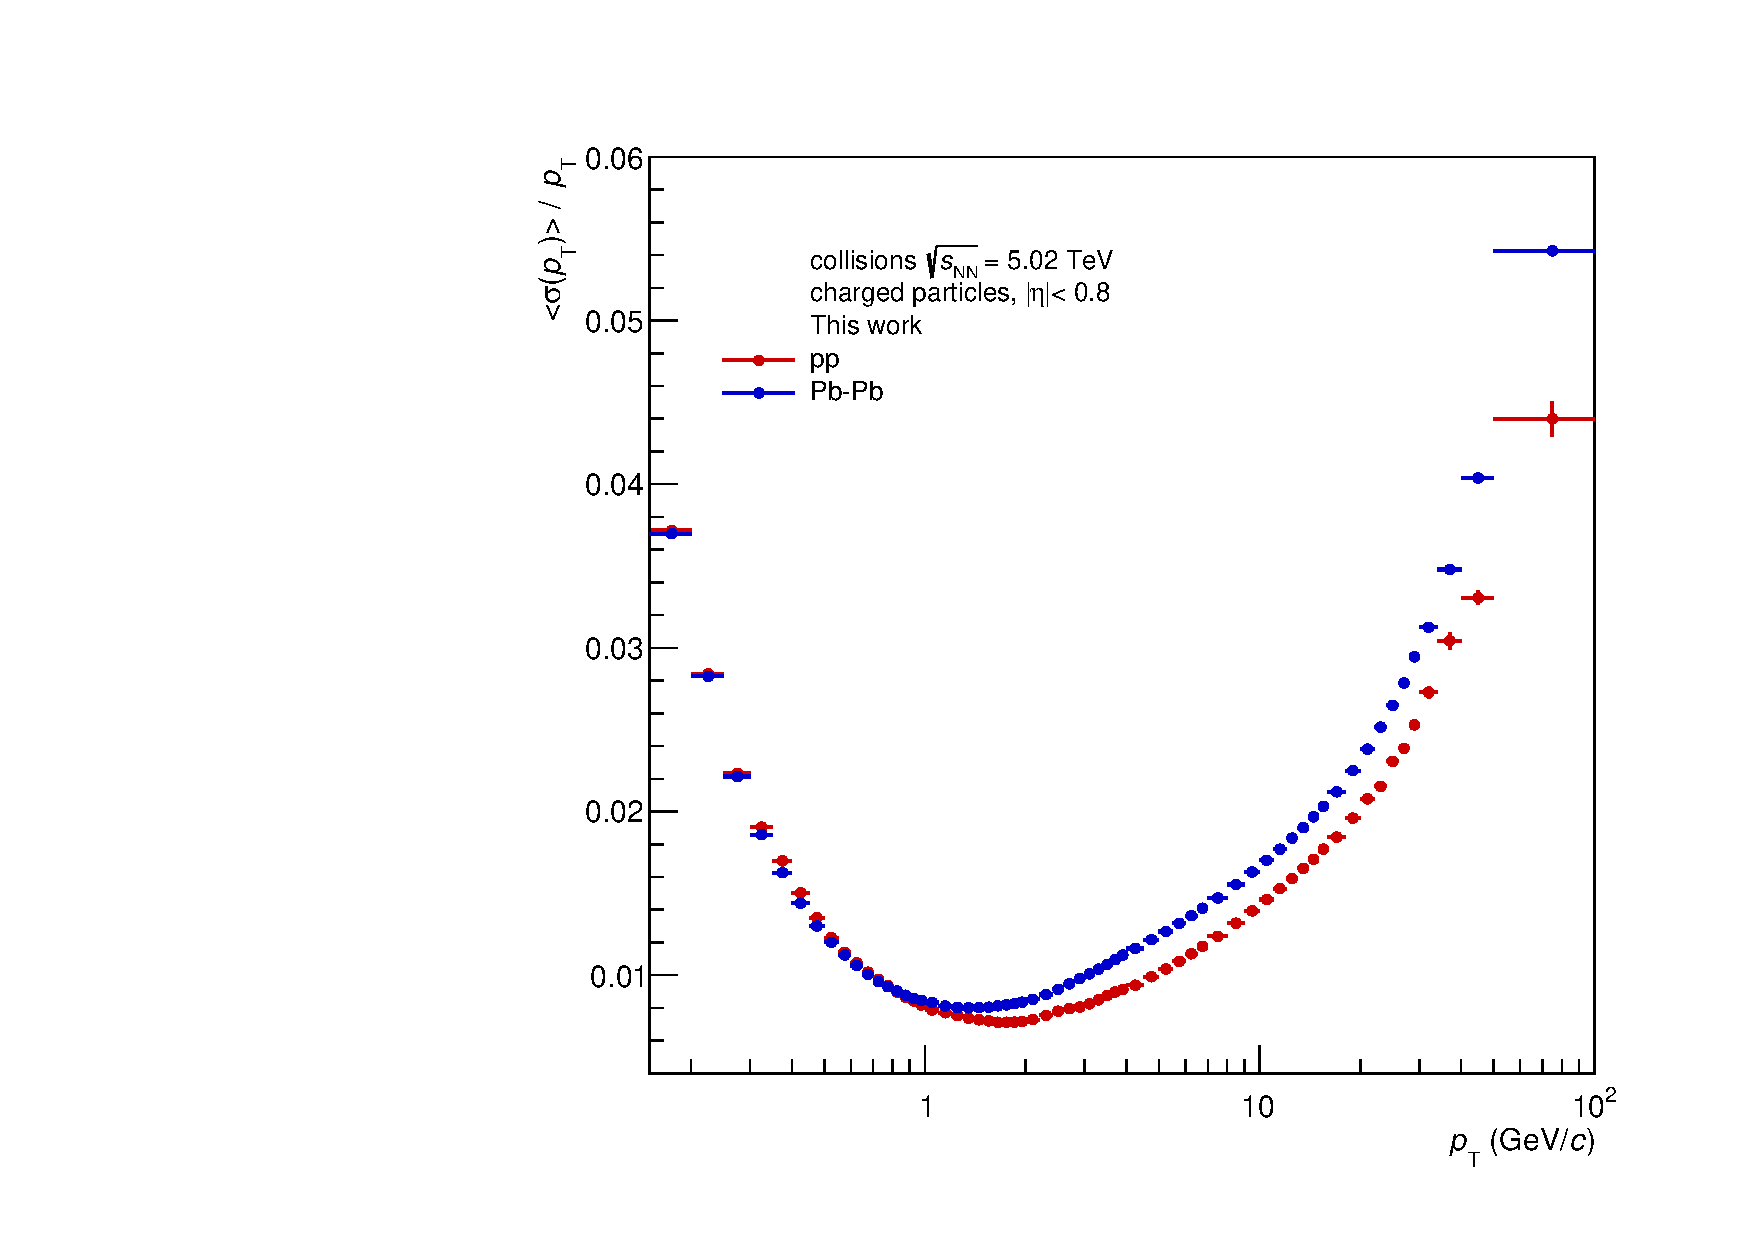
\includegraphics[width=12cm]{Plots/ptReso1D.pdf}  
\caption{The mean relative transverse momentum resolutions are obtained as function of the transverse momentum for pp and MB Pb-Pb collisions.}
\label{ptReso1D}
\end{figure}
\hspace{-0.3cm} As discussed in Section \ref{ptandmomreso}, the determination of the inverse of the transverse momentum is affected by a measurement uncertainty. Both track parameters are stored during the tracking procedure and can be used to determine the relative momentum resolution by means of Equation \ref{ptandmomreso}. In Figure \ref{ptReso2D}, the distribution of $\sigma(p_\text{T})/p_\text{T}$ is shown as function of \pt for the analysed pp collisions. The three visible structures at low \pt can be explained by the interaction of charged particles with the detector material of the ITS. When a particle crosses the detector, it undergoes multiple scattering and its trajectory is consequently deflected by small angles affecting thereby the track parameters determination. Such an effect is dependent on the particle mass and the observed distinct trends of the resolution correspond, in decreasing order of uncertainty, to protons, kaons and pions. For a more clear representation, the mean value $\langle\sigma(p_\text{T})/p_\text{T}\rangle$ of this distribution is calculated in each \pt interval. As result, the mean relative \pt resolution as function of $p_\text{T}$ is obtained as shown in Figure \ref{ptReso1D}. At low $p_\text{T}$, the relative $p_\text{T}$-resolutions are influenced mainly by the multiple scattering of the charged particles in the detector material. In this region, the results in pp and Pb-Pb as well as among the different centrality classes resemble each other as proved in (cit mknichel). At $p_\text{T} = 0.15$ GeV/$c$, the resolution is on average around 3.7\%.\\
The effect of the multiple scattering dissipates gradually until the distribution hits the minimum around 1.5 GeV/$c$ with a \pt resolution of approximately 0.7\% in pp and 0.8\% in Pb-Pb. At high $p_\text{T}$, charged particles experience a less pronounced curvature according to Equation \ref{radius}, which causes a deterioration of the spatial resolution. As consequence, the uncertainty grows linearly reaching values of 4.4\% in pp and 5.4\% in Pb-Pb.\\
Since the measurement of \pt is smeared due to the resolution, the \pt spectra must be corrected accordingly. While the smearing has a minor effect on the \pt spectra at low \pt given the smooth slope of the distributions, it becomes more pronounced in the high \pt region, where the \pt spectra describe a steeply falling shape. The corresponding correction is thus applied in the range $7 \leq p_\text{T} \leq 100$ GeV/$c$ by means of a $p_\text{T}$-dependent factor $c_\text{reso}$ calculated as follows: 
\begin{equation}
c_\text{reso}(p_\text{T}) = \dfrac{(\text{d}N/\text{d}p_\text{T})_\text{smeared}}{(\text{d}N/\text{d}p_\text{T})_\text{true}}
\label{ptresfactor}
\end{equation}
where the numerator corresponds to the measured \pt distribution, while the denominator is a \pt distribution free of smearing. As starting point, the \pt distributions from the previous ALICE publication, depicted in Section (cite theo. section), are used  given that they offer a good approximation of the true \pt distributions. For the calculation of $c_\text{reso}(p_\text{T})$, these \pt distributions are smeared using a simulation to emulate the effect of the \pt resolution on the \pt distributions. The details of this procedure are outlined in the following.
\subsubsection{Calculation of the correction factor}
\begin{figure}[tb!]
\centering
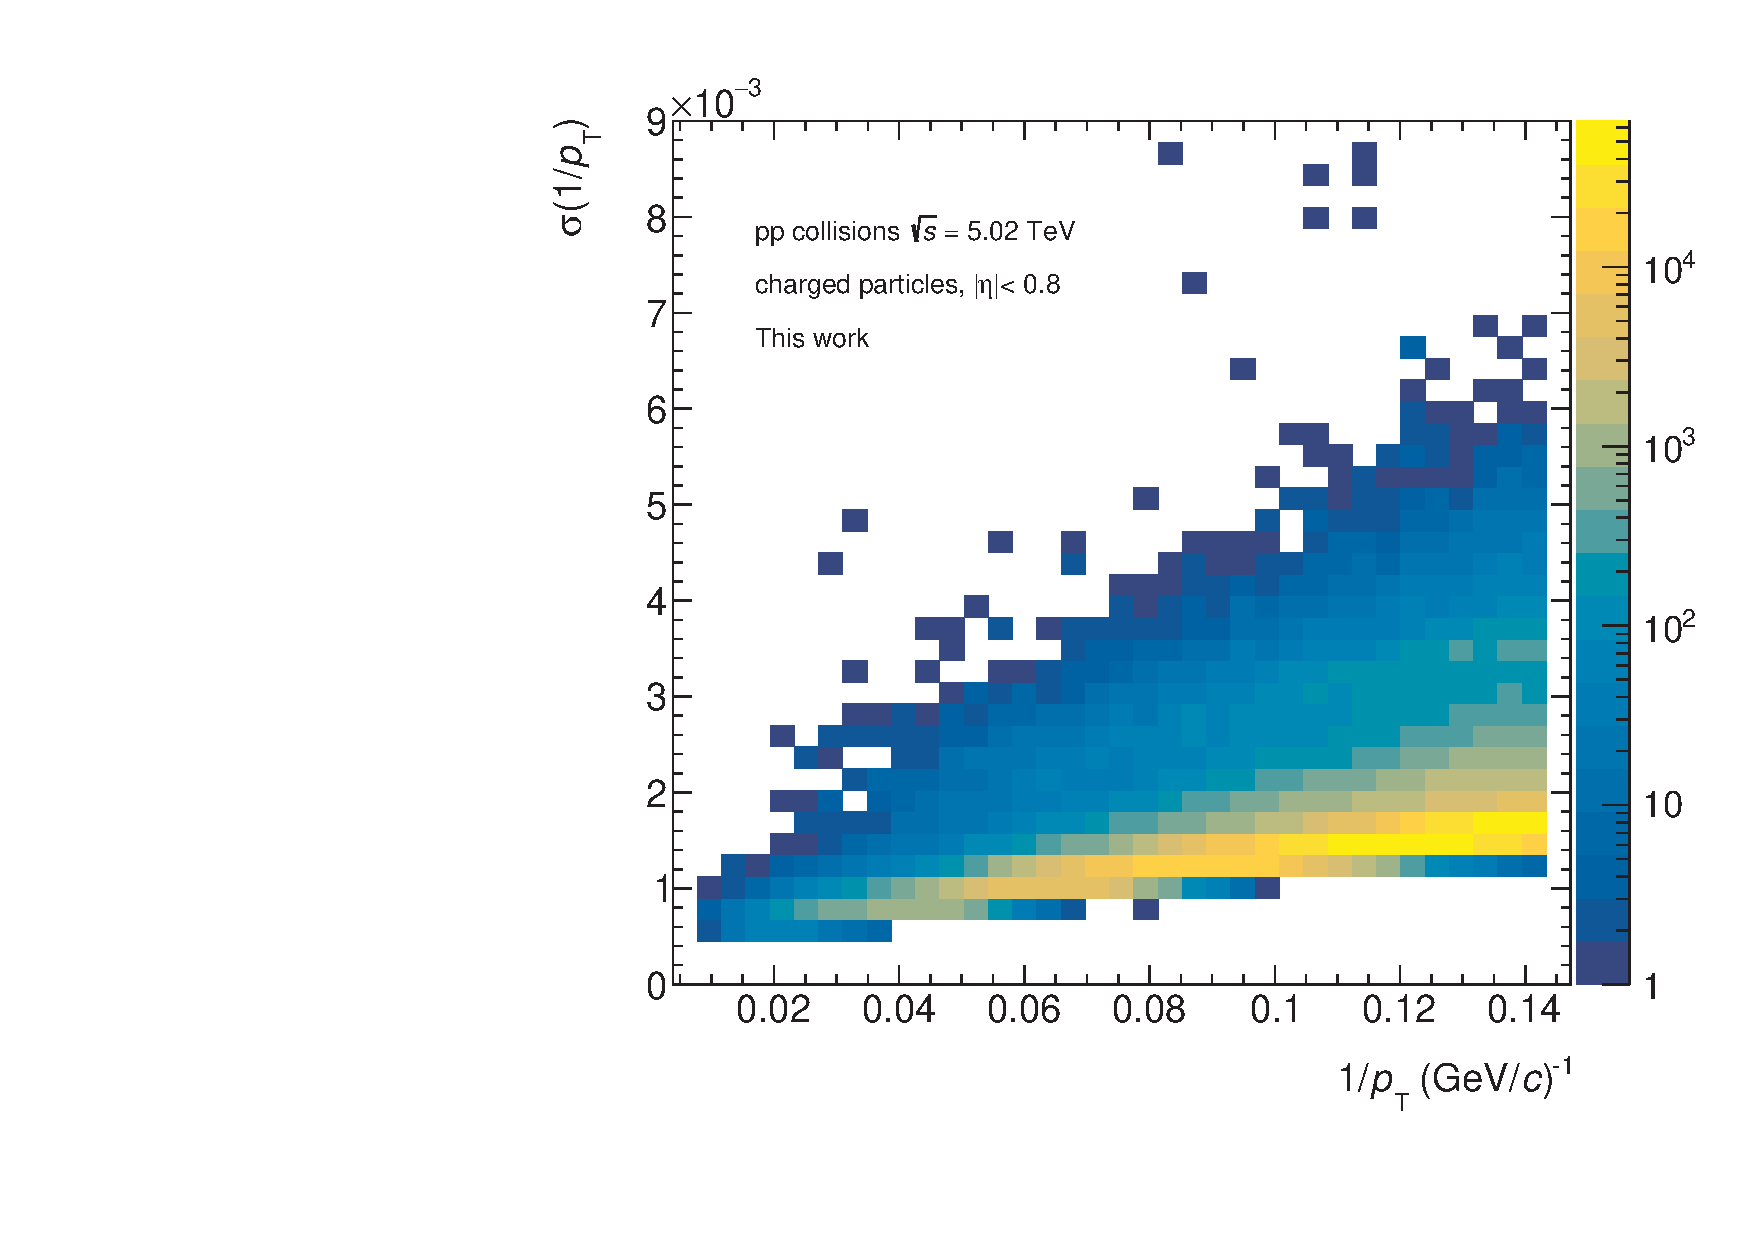
\includegraphics[width=0.495\textwidth]{Plots/reso2dim.pdf}  
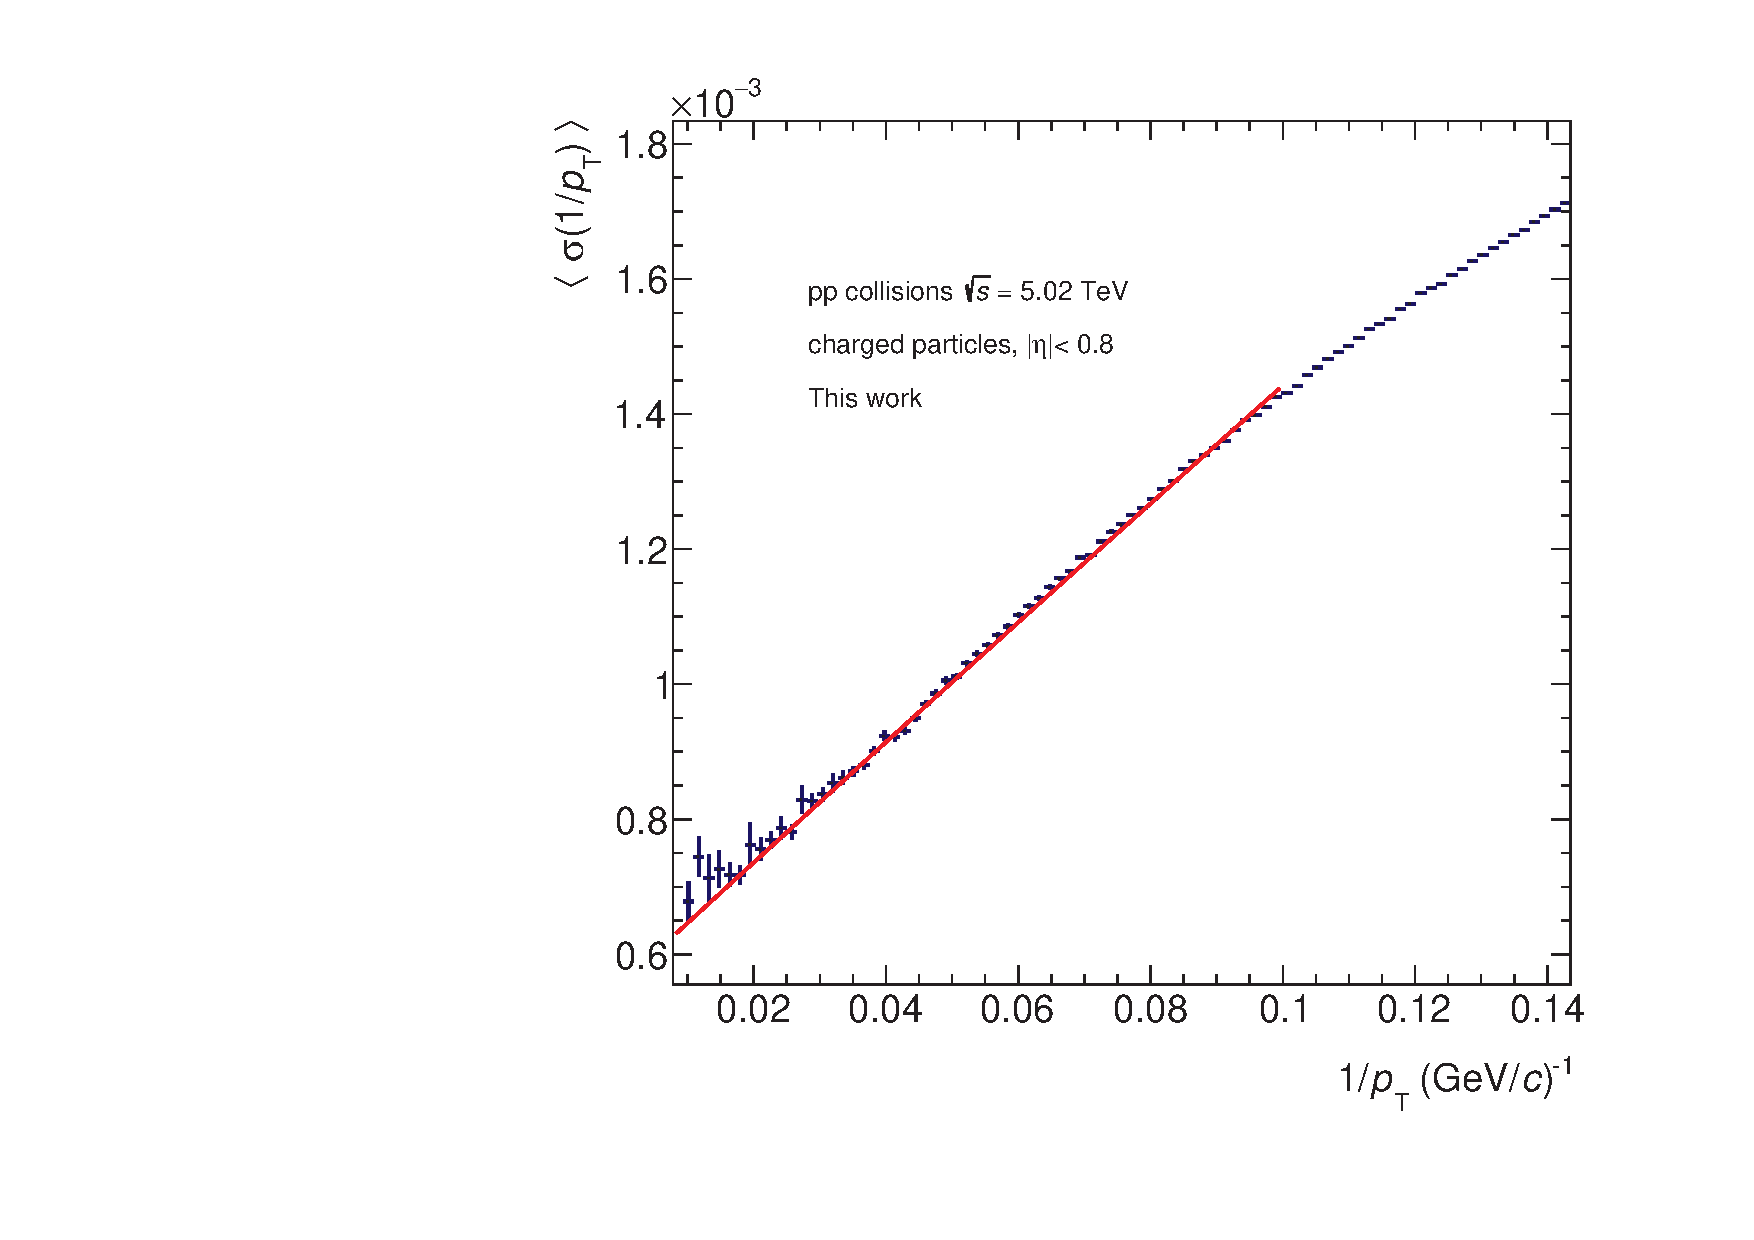
\includegraphics[width=0.495\textwidth]{Plots/fitfunc.pdf}  
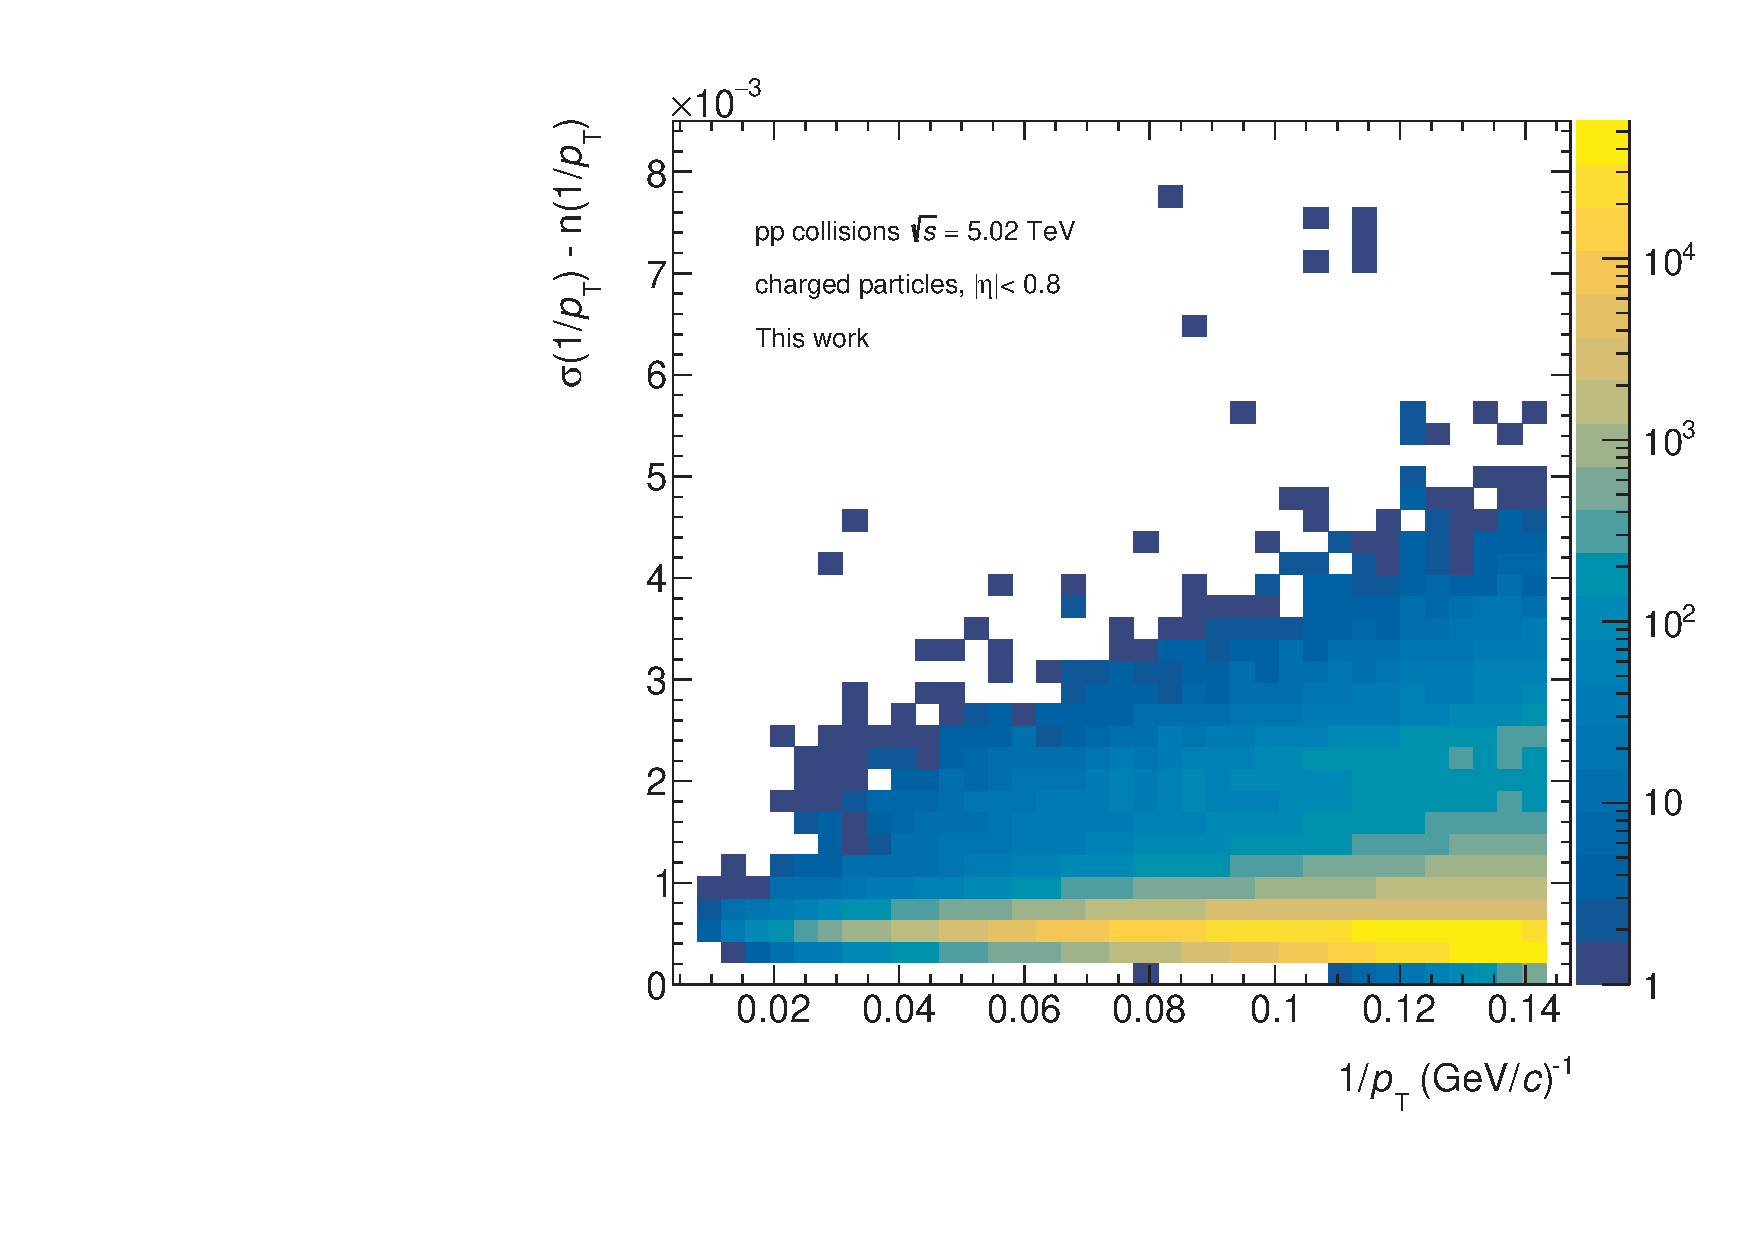
\includegraphics[width=0.495\textwidth]{Plots/scaledcov.pdf}  
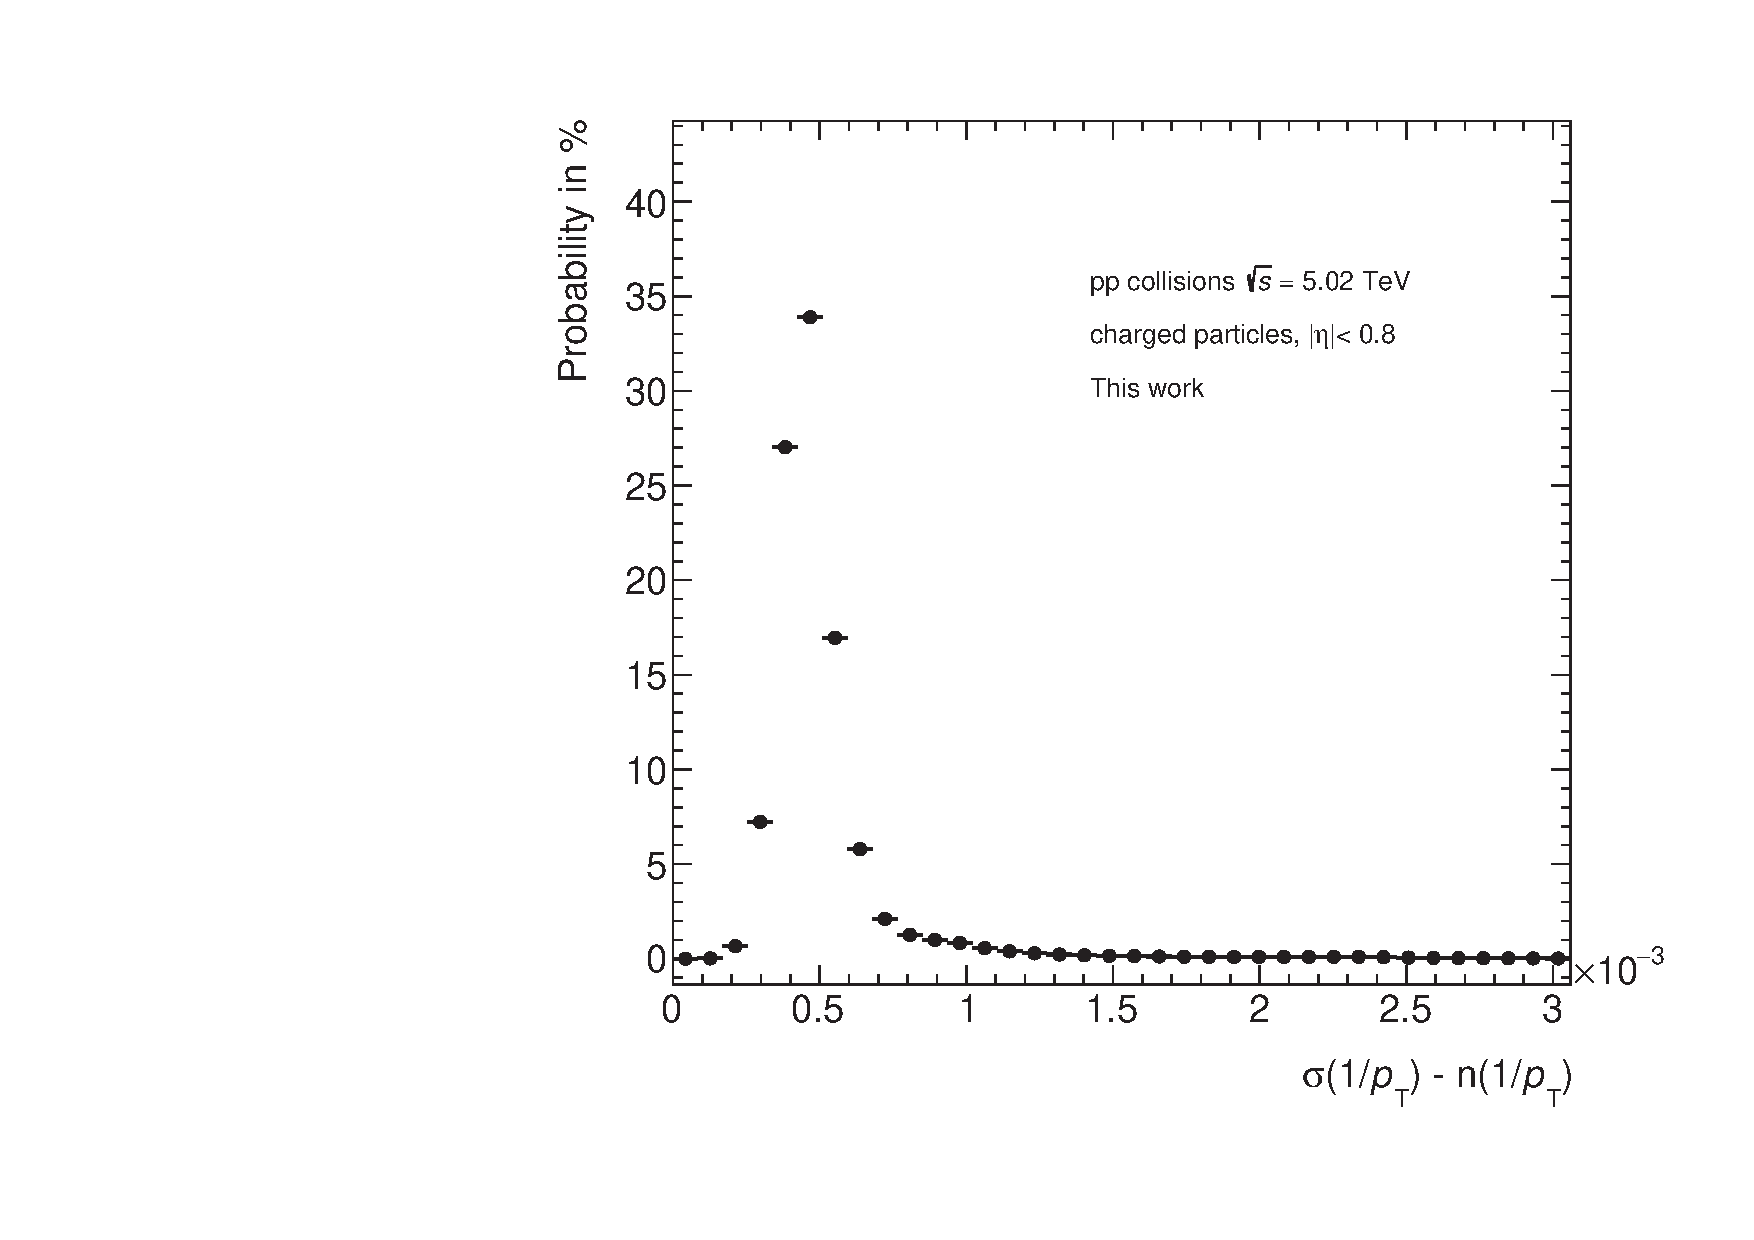
\includegraphics[width=0.495\textwidth]{Plots/probabilitydist.pdf}  
\caption{\textbf{Top.} Left: Two-dimensional distribution of the uncertainty on the inverse of the transverse momentum $\sigma(1/p_{\mathrm{T}})$ as function of $1/p_{\mathrm{T}}$. Right: 2nd order polynomial parametrization $n(1/p_{\mathrm{T}})$ of the mean uncertainty $\langle\sigma(1/p_\text{T})\rangle$ as function of $1/p_{\mathrm{T}}$. \textbf{Bottom.} Left: Two-dimensional distribution of the scaled uncertainty $\sigma(1/p_{\mathrm{T}})$ as function of $1/p_{\mathrm{T}}$. Right: Probability function of $\sigma(1/p_\text{T})$ obtained after projecting the scaled uncertainty into the $y$-axis.}
\label{4plots}
\end{figure}
\begin{figure}[htb!]
\centering
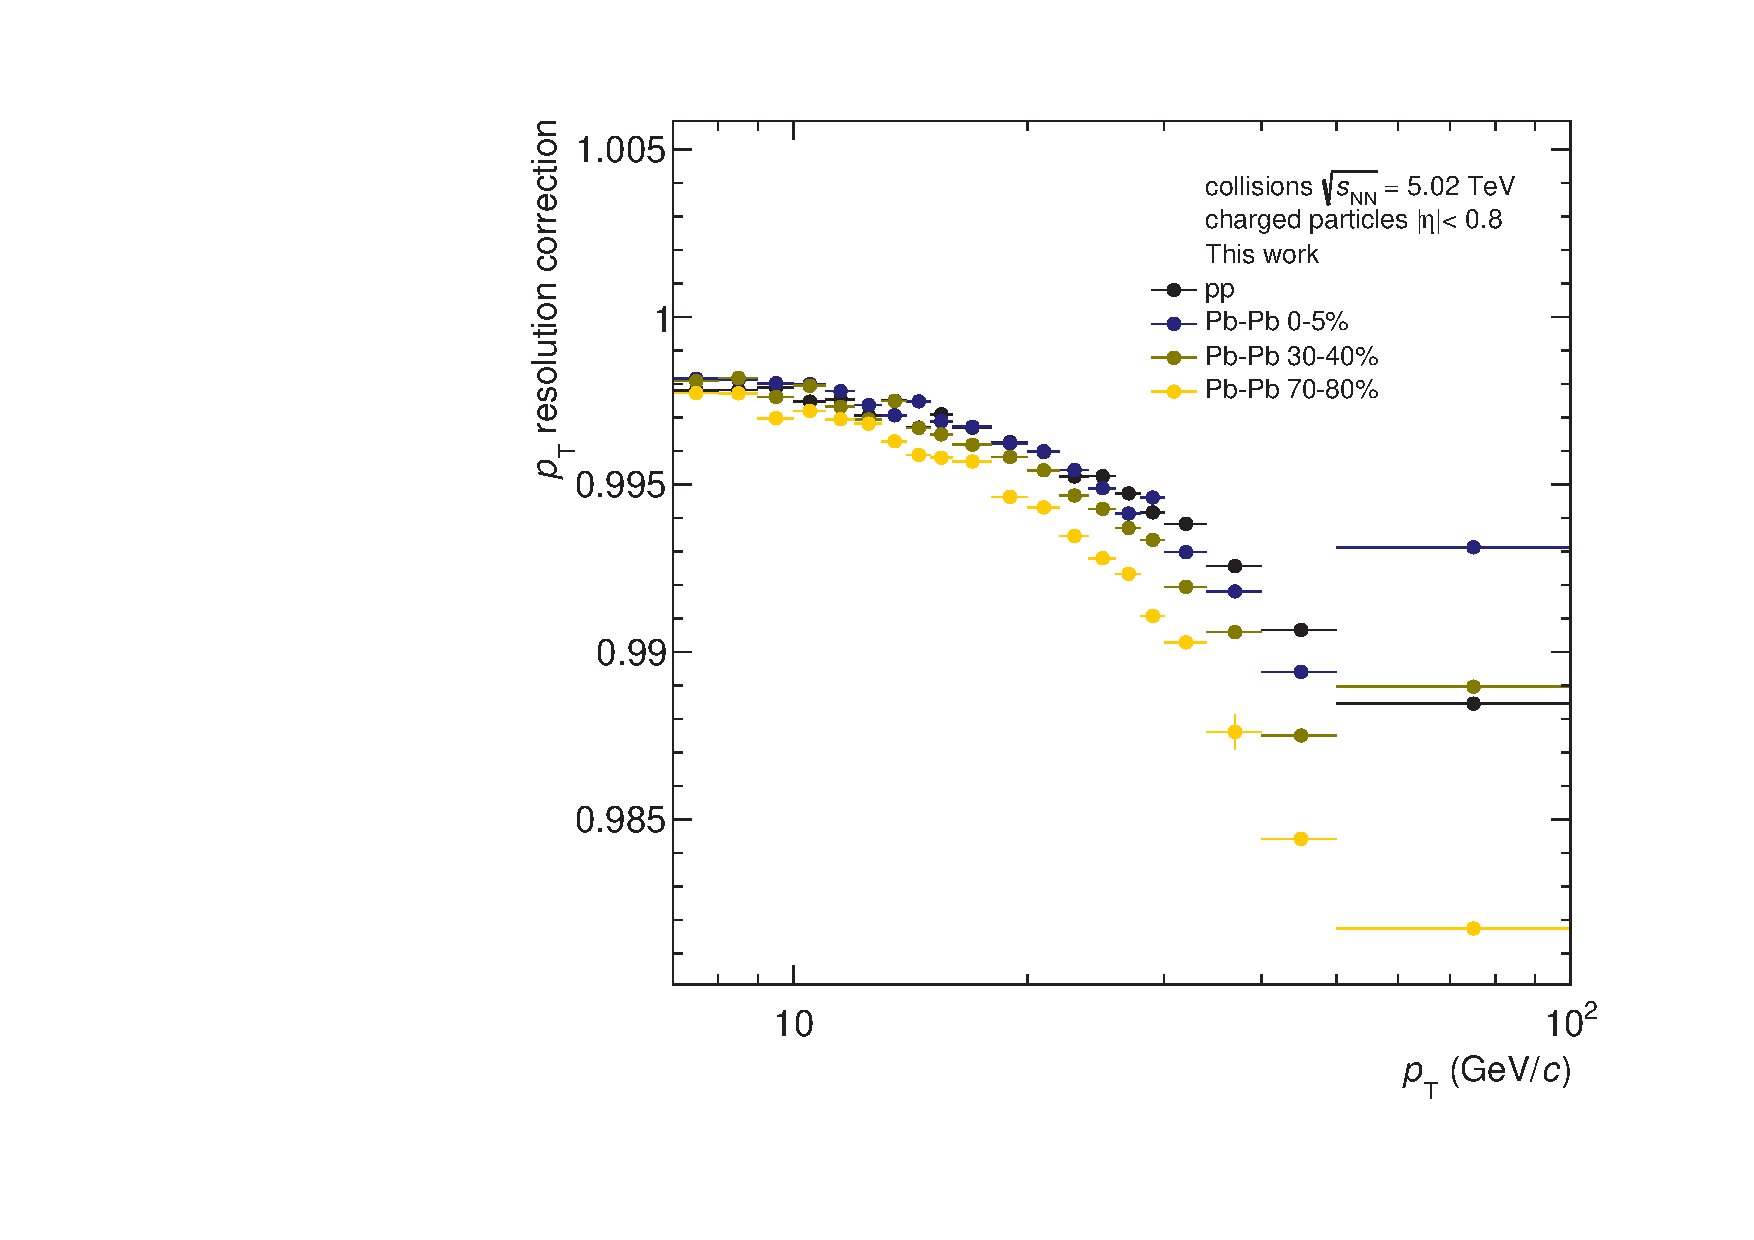
\includegraphics[width=12cm]{Plots/ptrescorrppPbPb.pdf}  
\caption{\pt resolution correction factor as function of $p_{\mathrm{T}}$ in pp and in three centrality classes of Pb-Pb collisions at $\sqrt{s_\text{NN}} = 5.02$ TeV recorded in ALICE.}
\label{ptrescorrppPbPb}
\end{figure}
The smearing is carried out through a simulation that uses as input a sample of filtered high \pt tracks that underwent the same track requirements as summarized in Table \ref{tab:Cuts}. The parameter $\sigma(1/p_\text{T})$ of these tracks is obtained as function of $1/p_\text{T}$ as shown in the top-left panel of Figure \ref{4plots} for the case of pp collisions. This two-dimensional representation is converted to a distribution of the mean uncertainty $\langle\sigma(1/p_\text{T})\rangle$ as function of $1/p_\text{T}$. Next, this distribution is parametrized with a 2nd order polynomial $n(1/p_\text{T})$ which is subtracted from the original uncertainty $\sigma(1/p_\text{T})$ to exclude the \pt dependence and, by that, reduce statistical fluctuations as seen in the top-right panel of Figure \ref{4plots}. The scaled $\sigma(1/p_\text{T})$ distribution (see bottom left panel of Figure \ref{4plots}) is subsequently projected into the $y$-axis obtaining thereby a distribution that reveals the probability function of $\sigma(1/p_\text{T})$ as shown in the bottom-right panel of Figure \ref{4plots}.\\
After determining the shape of $\sigma(1/p_\text{T})$ without the \pt dependence, the smearing is performed. In this process, simulated tracks are distributed according to a power-law fit of the true \pt distributions in the range $7 \leq p_\text{T} \leq 100$ GeV/$c$. These are then transformed in $1/p_\text{T}$ distributions. Each $1/p_\text{T}$ value is smeared according to a Gaussian with a standard deviation generated randomly based on the probability function of $\sigma(1/p_\text{T})$. This standard deviation is then adjusted adding a factor extracted from an evaluation of the polynomial $n(1/p_\text{T})$ as recorrection for the above mentioned suppression of statistical fluctuations (see bottom-left panel of Figure \ref{4plots} ). Finally, the smeared $1/p_\text{T}$ distribution is reconverted in a \pt spectrum.\\
In Figure \ref{ptrescorrppPbPb}, the resulting correction factors as defined in Equation \ref{ptresfactor} for pp and for central, semi-central and peripheral Pb-Pb collisions are illustrated. The correction factor falls monotonically and the effect finds its maximum at the largest \pt interval with a percentage value of around 1.2\% (1\%) for pp (Pb-Pb) collisions. The Pb-Pb results show a similar trend as in the pp data collection. Nevertheless, a centrality dependence of the correction factors is observed which originates from the different steepness of the true \pt spectra.
\section{Implementation of the corrections}
\label{secCorr}
As already mentioned, the track-level corrections affect the shape of the primary track distribution $N(p_\text{T})$. The corrected primary track distribution $N_\text{corr}(p_\text{T})$ can be defined as follows:
\begin{equation}
\begin{split}
N_\text{corr}(p_\text{T}) = &  N_\text{raw}(p_\text{T}) \times \dfrac{1}{\epsilon(p_\text{T}) \cdot c_\text{par comp}(p_\text{T})} \\
& \times (1 - c_\text{cont}(p_\text{T}) \cdot c_\text{sec. sca.}(p_\text{T})) \\
&\times \dfrac{1}{c_\text{reso}(p_\text{T})} \times \dfrac{1}{\chi_\text{sig loss}(p_\text{T})} 
\end{split}
\end{equation}
where $\epsilon(p_\text{T})$ is the tracking efficiency, $c_\text{par comp}(p_\text{T})$ the particle composition correction, $c_\text{cont}(p_\text{T})$ the secondary contamination correction, $c_\text{sec sca}(p_\text{T})$ the secondary scaling, $c_\text{reso}(p_\text{T})$ the \pt resolution correction and $\chi_\text{sig loss}(p_\text{T})$ the signal loss, which is only applied in pp collisions. The implementation of this equations leads to the full corrected \pt distributions in pp and Pb-Pb collisions. According to the definition of the nuclear modification factor, the results in pp collisions are expressed in form of a differential cross section: 
\begin{equation}
\label{EqdiffCross}
\dfrac{\text{d}^2 \sigma^\text{pp}_\text{ch} }{\text{d}\eta \text{d}p_\text{T}} = \sigma_\text{vis} \cdot \dfrac{1}{N_\text{INEL}} \cdot \dfrac{\text{d}^2 N^\text{pp}	_\text{corr}}{\text{d}\eta \text{d}p_\text{T}}
\end{equation}
where $N_\text{INEL}$ corresponds to the total number of inelastic events and $\sigma_\text{vis}$ the visible inelastic cross section discussed in Section \ref{Norm}. In the case of Pb-Pb collisions, the physical quantity used for the determination of nuclear modification factors is the invariant yield which is calculated as follows
\begin{equation}
\label{Eqinyield}
\dfrac{\text{d}^2 N^\text{Pb-Pb}_\text{ch}}{\text{d}\eta \text{d}p_\text{T}} = \dfrac{1}{N_\text{INEL}} \cdot \dfrac{\text{d}^2 N^\text{Pb-Pb}_\text{corr}}{\text{d}\eta \text{d}p_\text{T}}
\end{equation}
The differentials $\text{d}\eta$ and $\text{d}p_\text{T}$ in Equations \ref{EqdiffCross} and \ref{Eqinyield} are approximated with the full $\eta$-range $\Delta \eta = 1.6$ and the width of the \pt interval $\Delta p_\text{T}$, respectively.
\section{Systematic uncertainties}
MC simulations aim to reproduce accurately the detector performance so that their information can be used to correct the data. However, the simulations are subject to uncertainties which affect the MC based corrections and therefore the \pt distributions as well as the nuclear modification factors. These are the so-called systematic uncertainties. In this thesis, the source of systematic uncertainties considered arises from the track selection criteria. However, other sources of systematic uncertainties have been identified in previous measurements of nuclear modification factors (cite paper). In this chapter, these other sources will be described and their impact on the \pt distributions presented, but they will not be applied to the final results shown in this thesis.
\subsection{Track selection} 
\label{systracksel}
\begin{figure}[!htb]
\centering
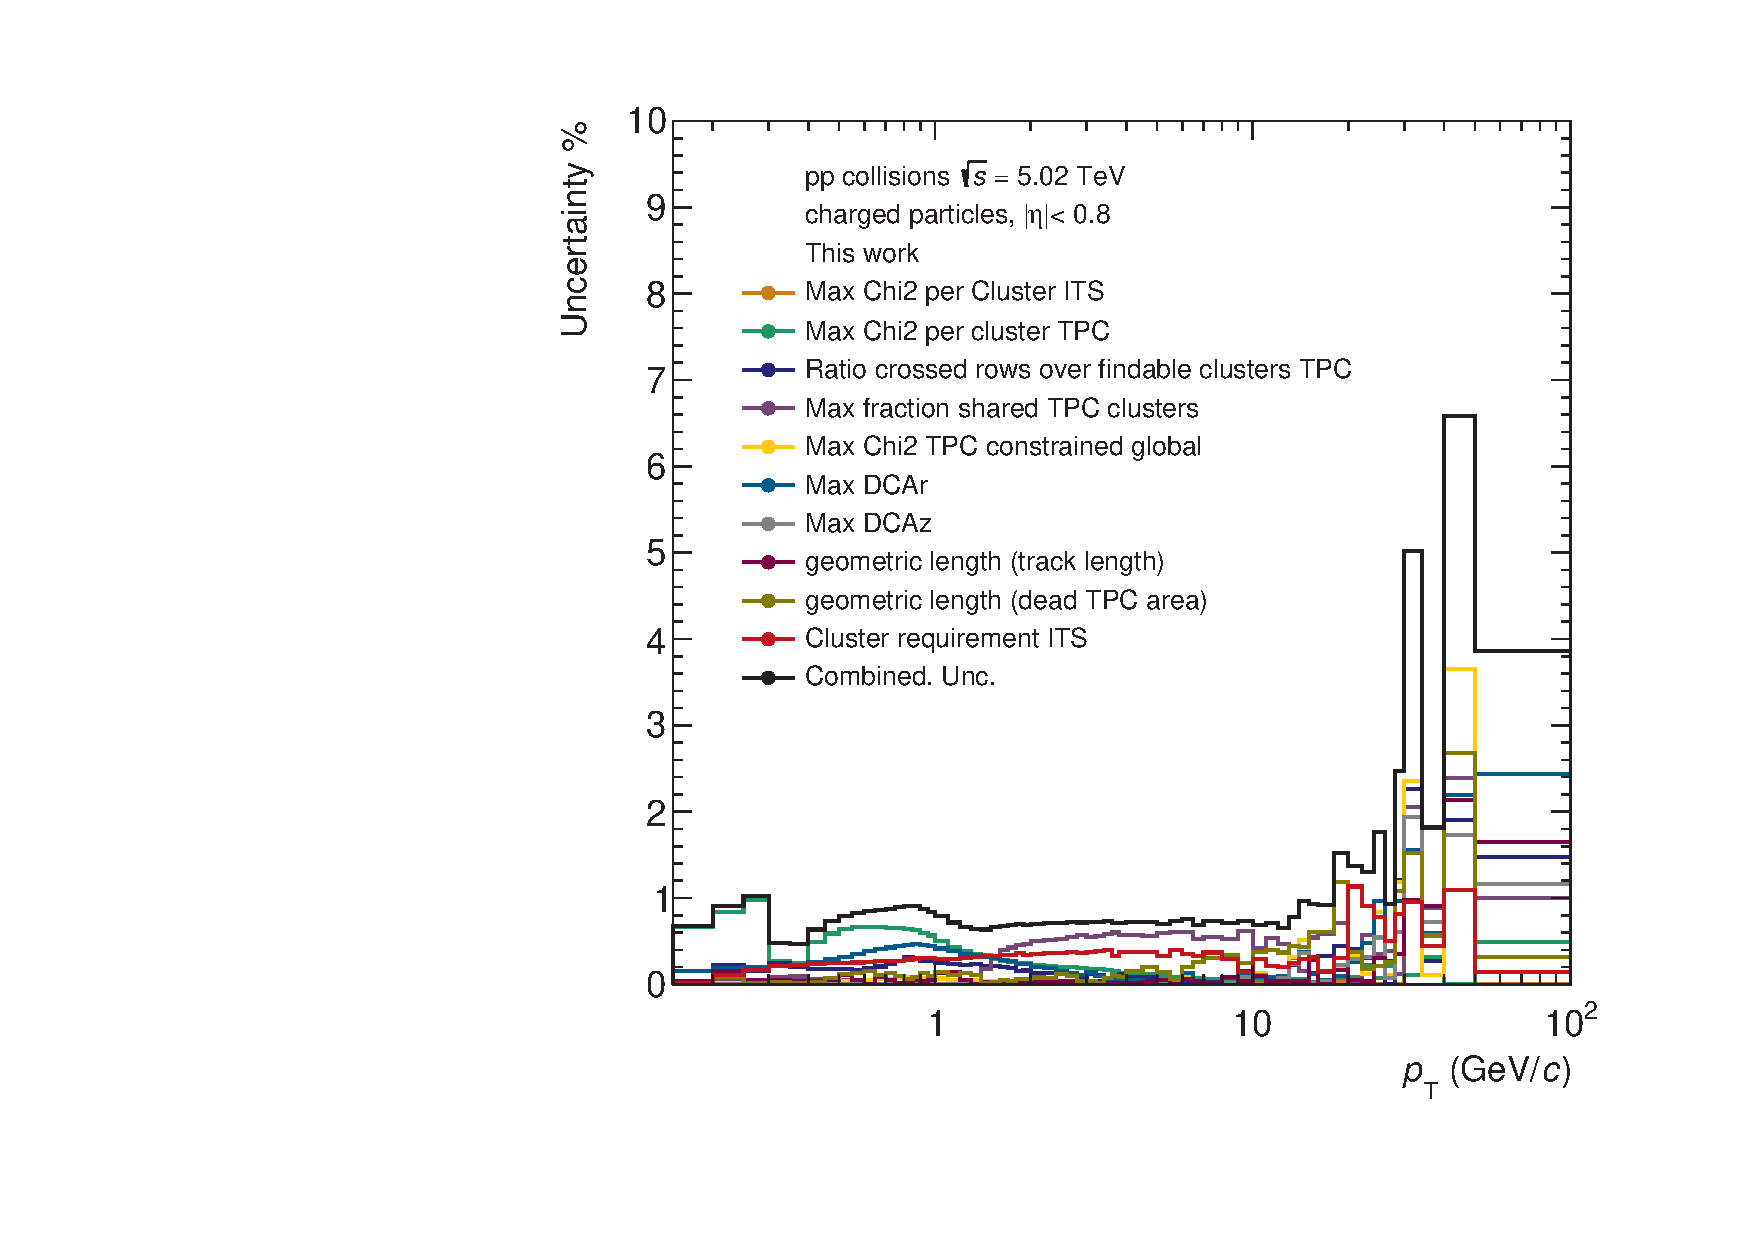
\includegraphics[width=0.495\textwidth]{Plots/SysUncpp.pdf}  
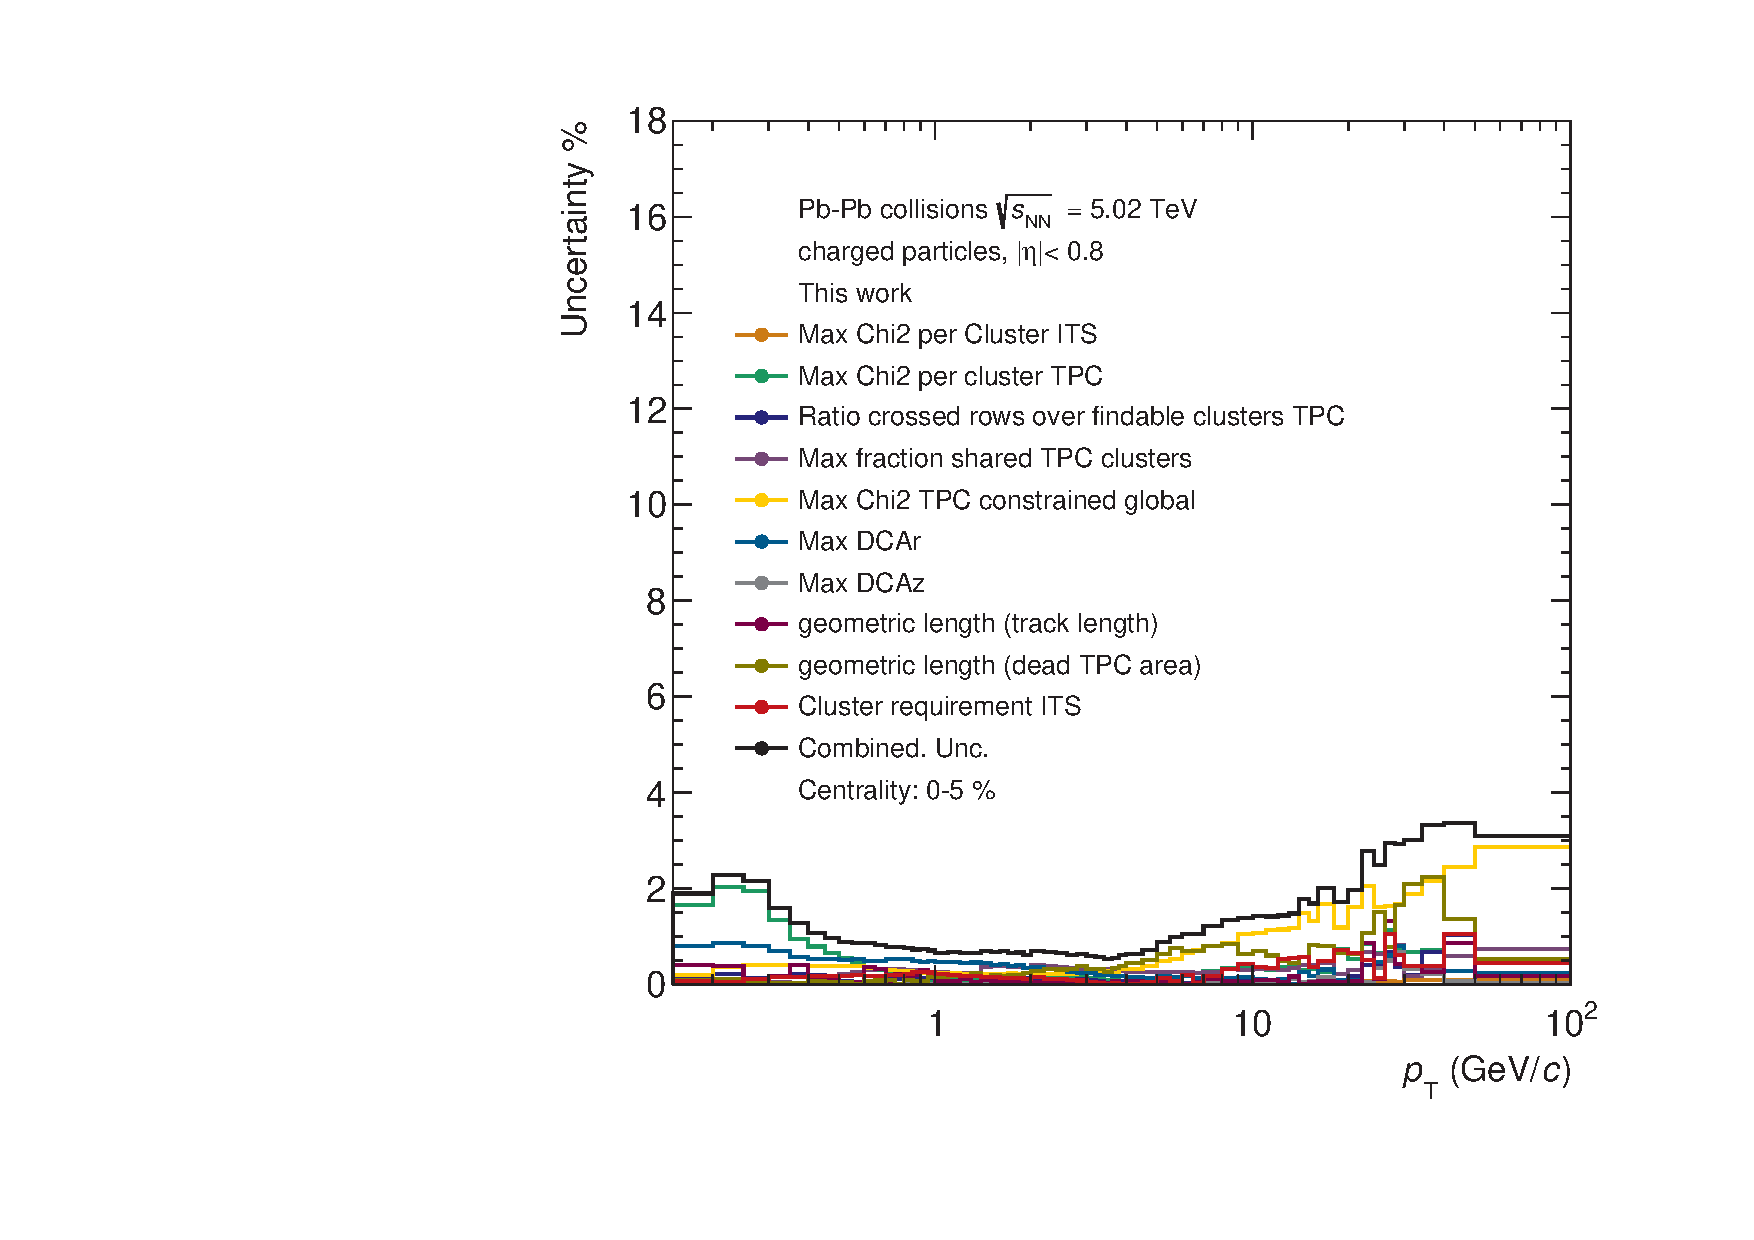
\includegraphics[width=0.495\textwidth]{Plots/SysUncPbPbcent.pdf}  
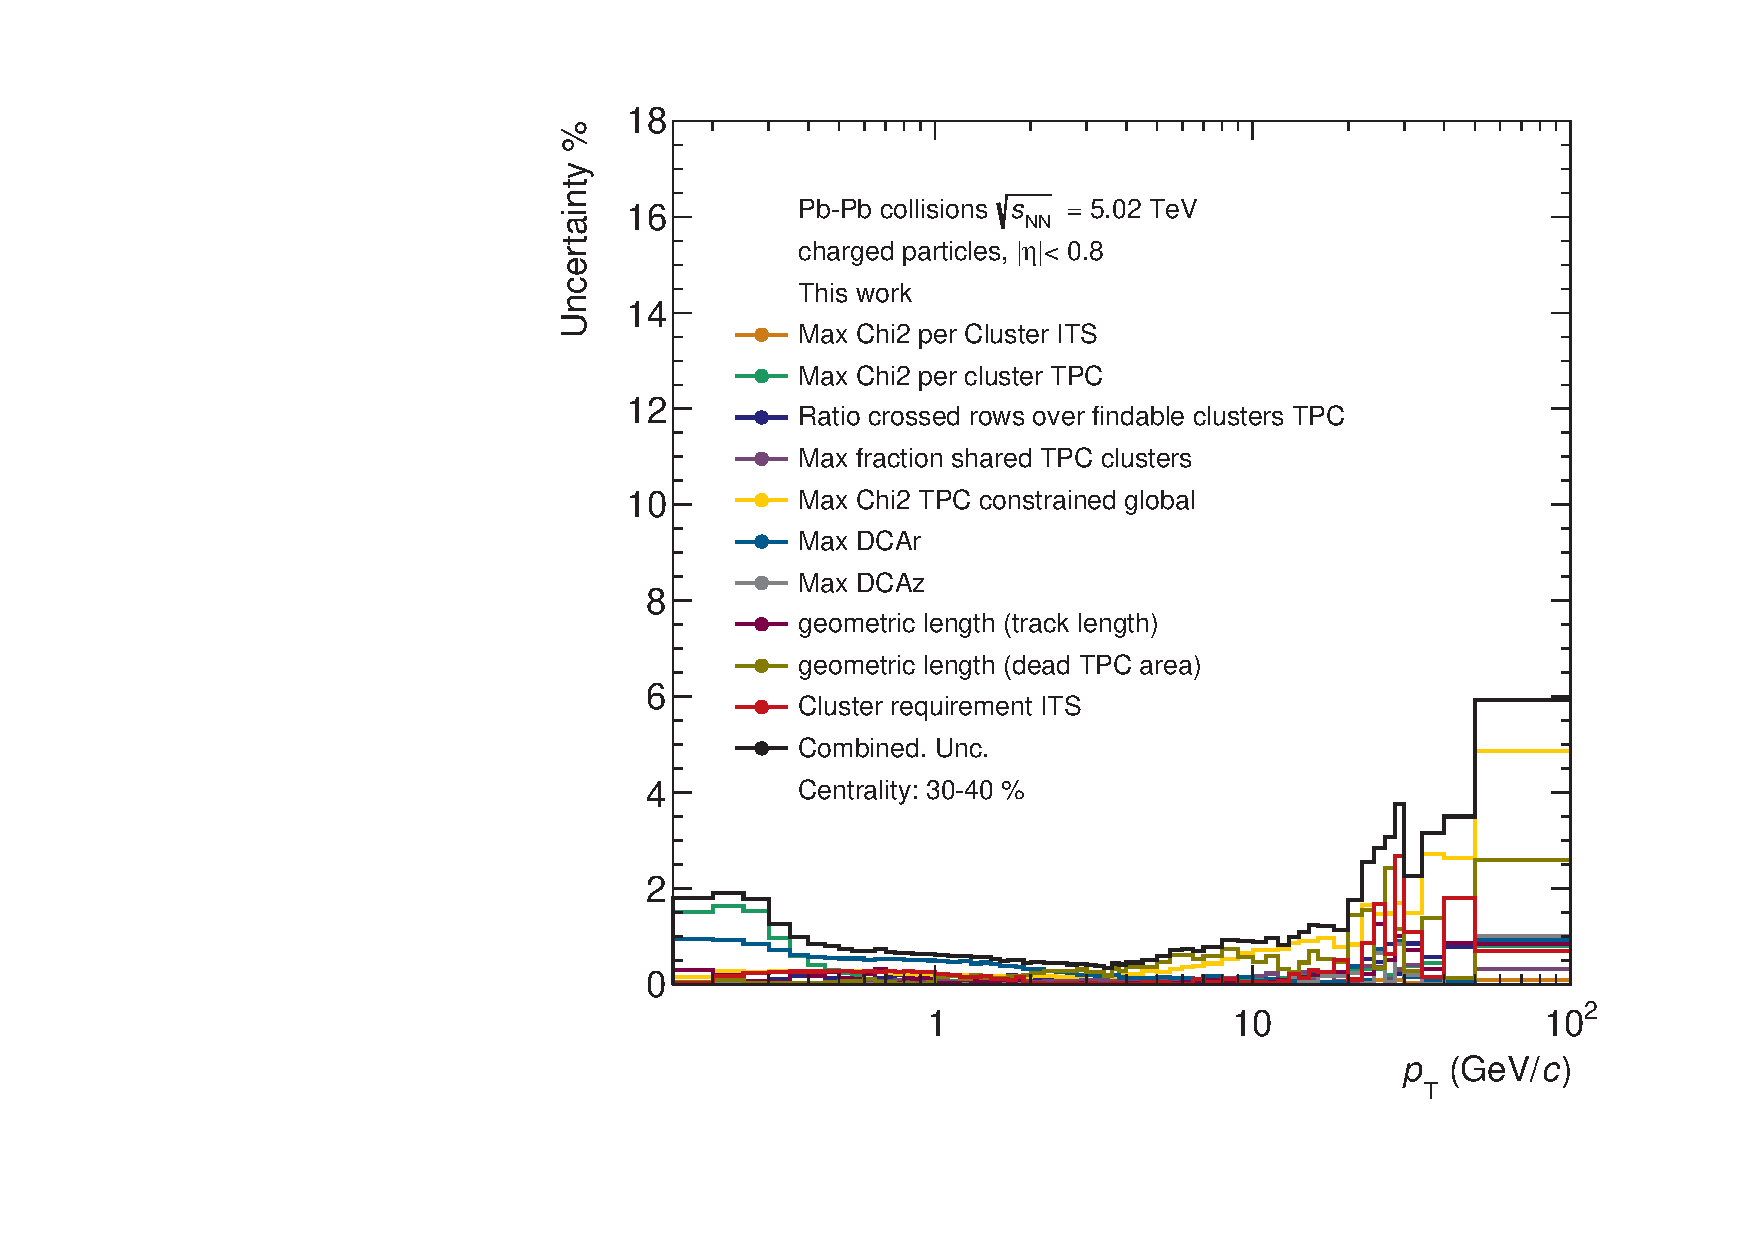
\includegraphics[width=0.495\textwidth]{Plots/SysUncPbPbsemi.pdf}  
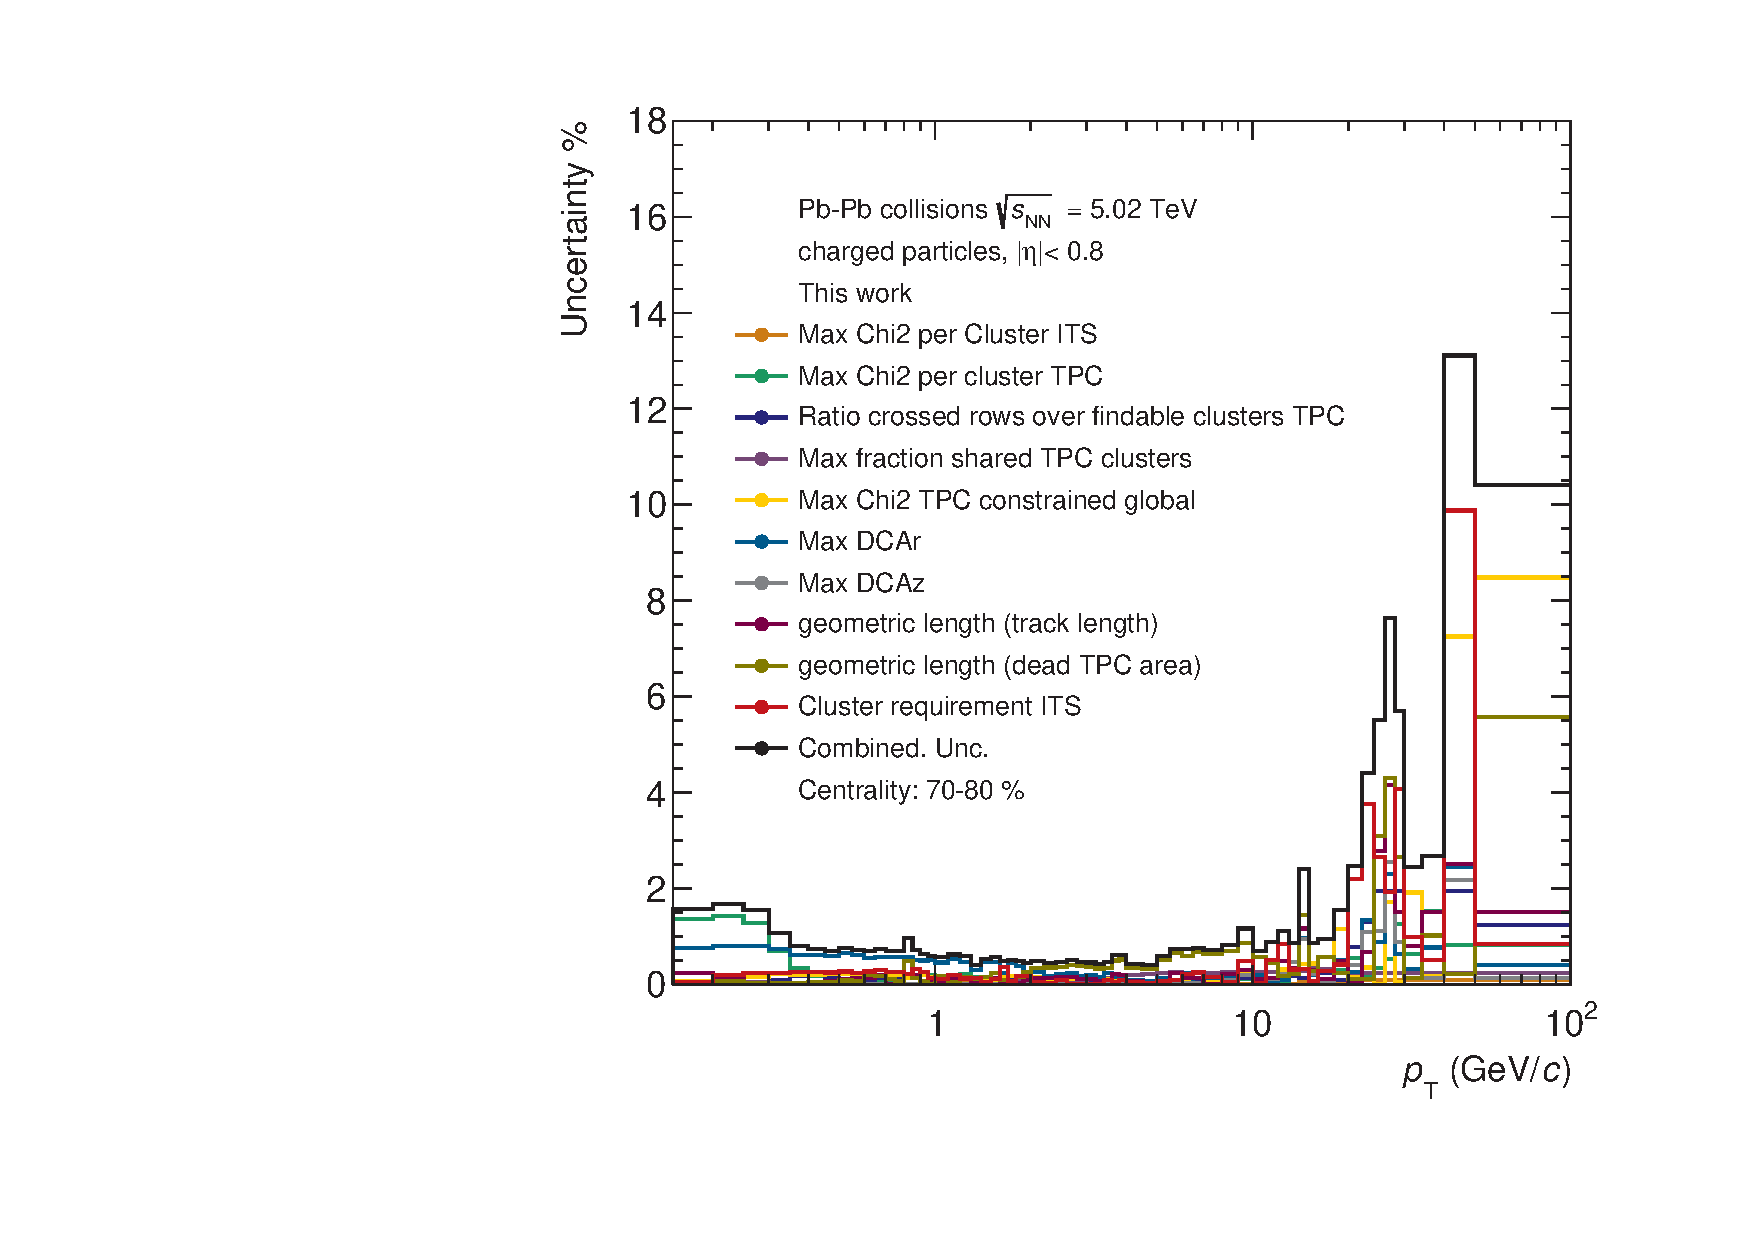
\includegraphics[width=0.495\textwidth]{Plots/SysUncPbPbperi.pdf}  
\caption{Relative systematic uncertainties of the \pt spectra from the track selection for pp as well as central, semi-central and peripheral Pb-Pb collisions.}
\label{SysUncSpec}
\end{figure}
\begin{figure}[!htb]
\centering
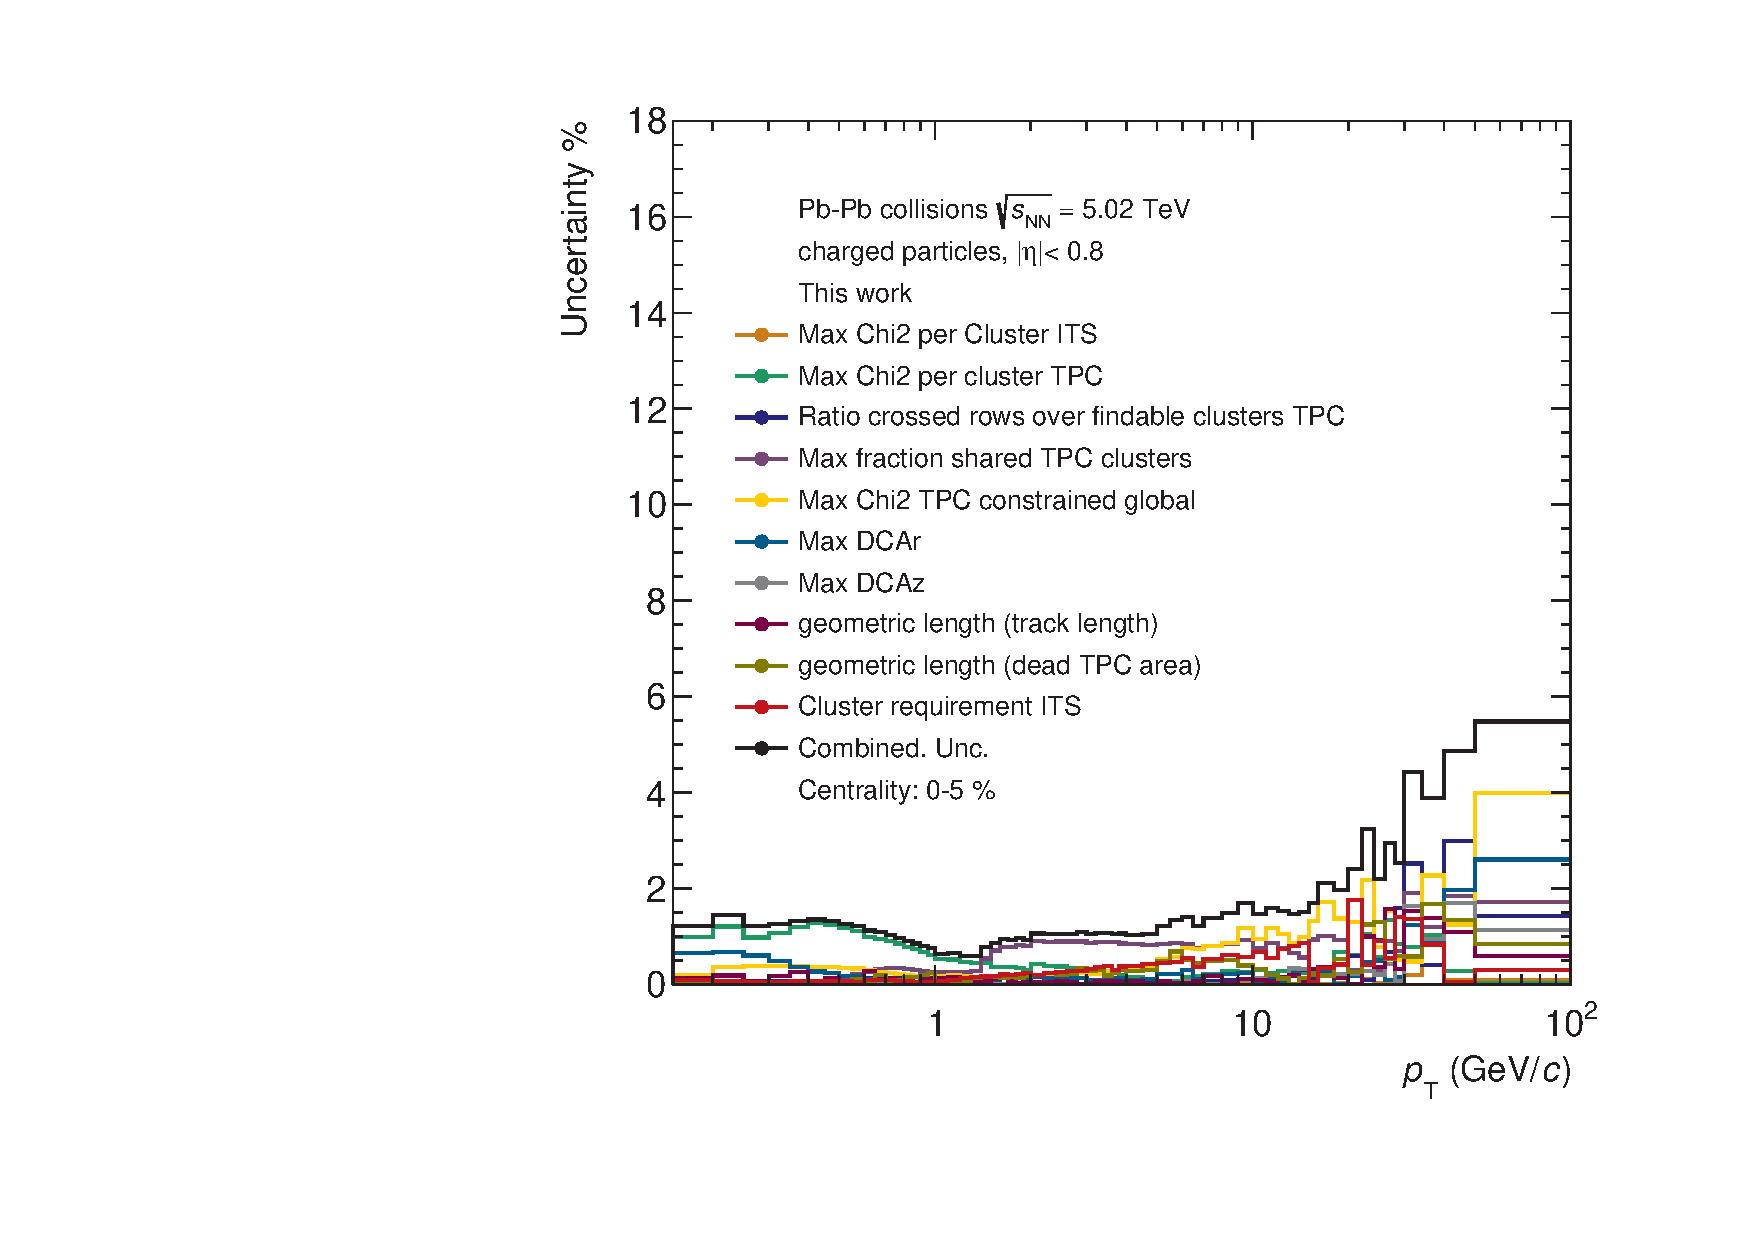
\includegraphics[width=0.495\textwidth]{Plots/SysUncRaacent.pdf}  
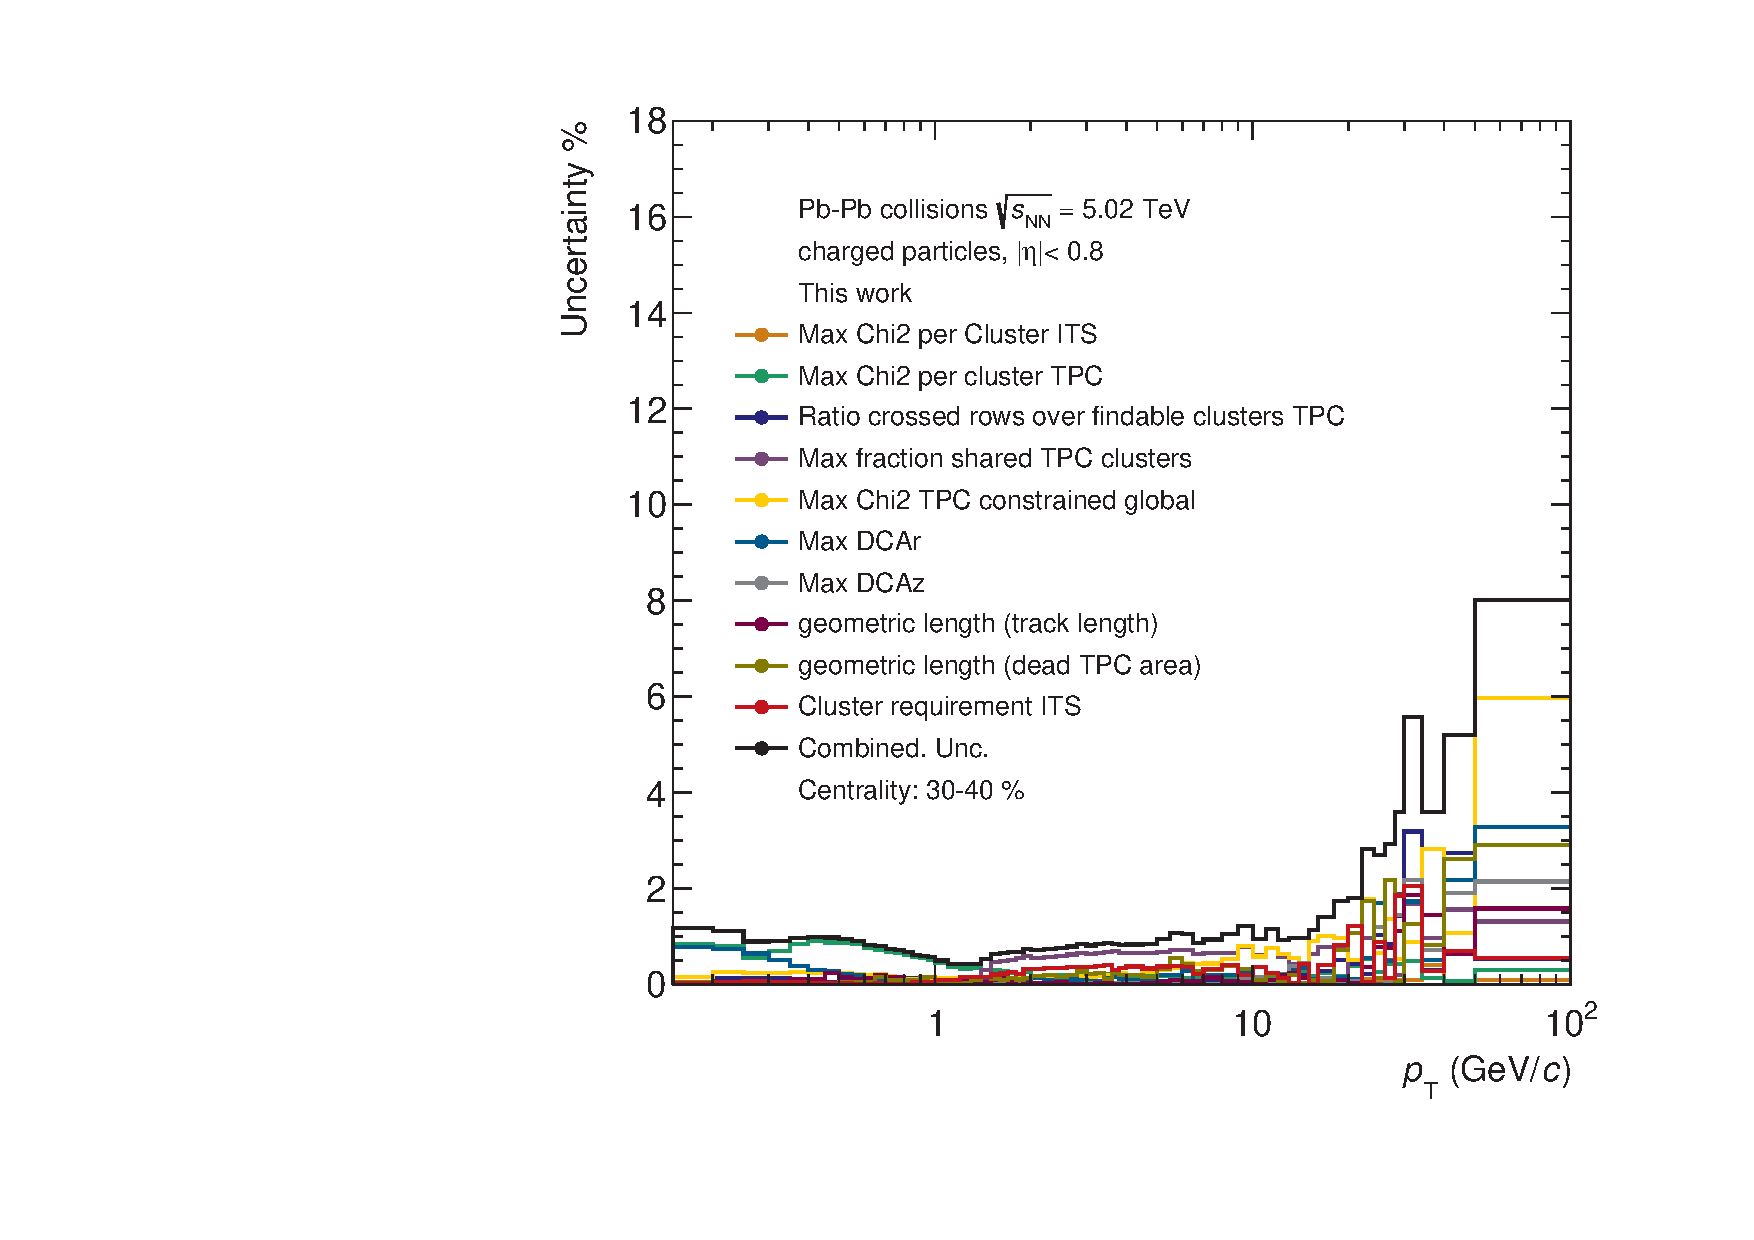
\includegraphics[width=0.495\textwidth]{Plots/SysUncRaasemi.pdf}  
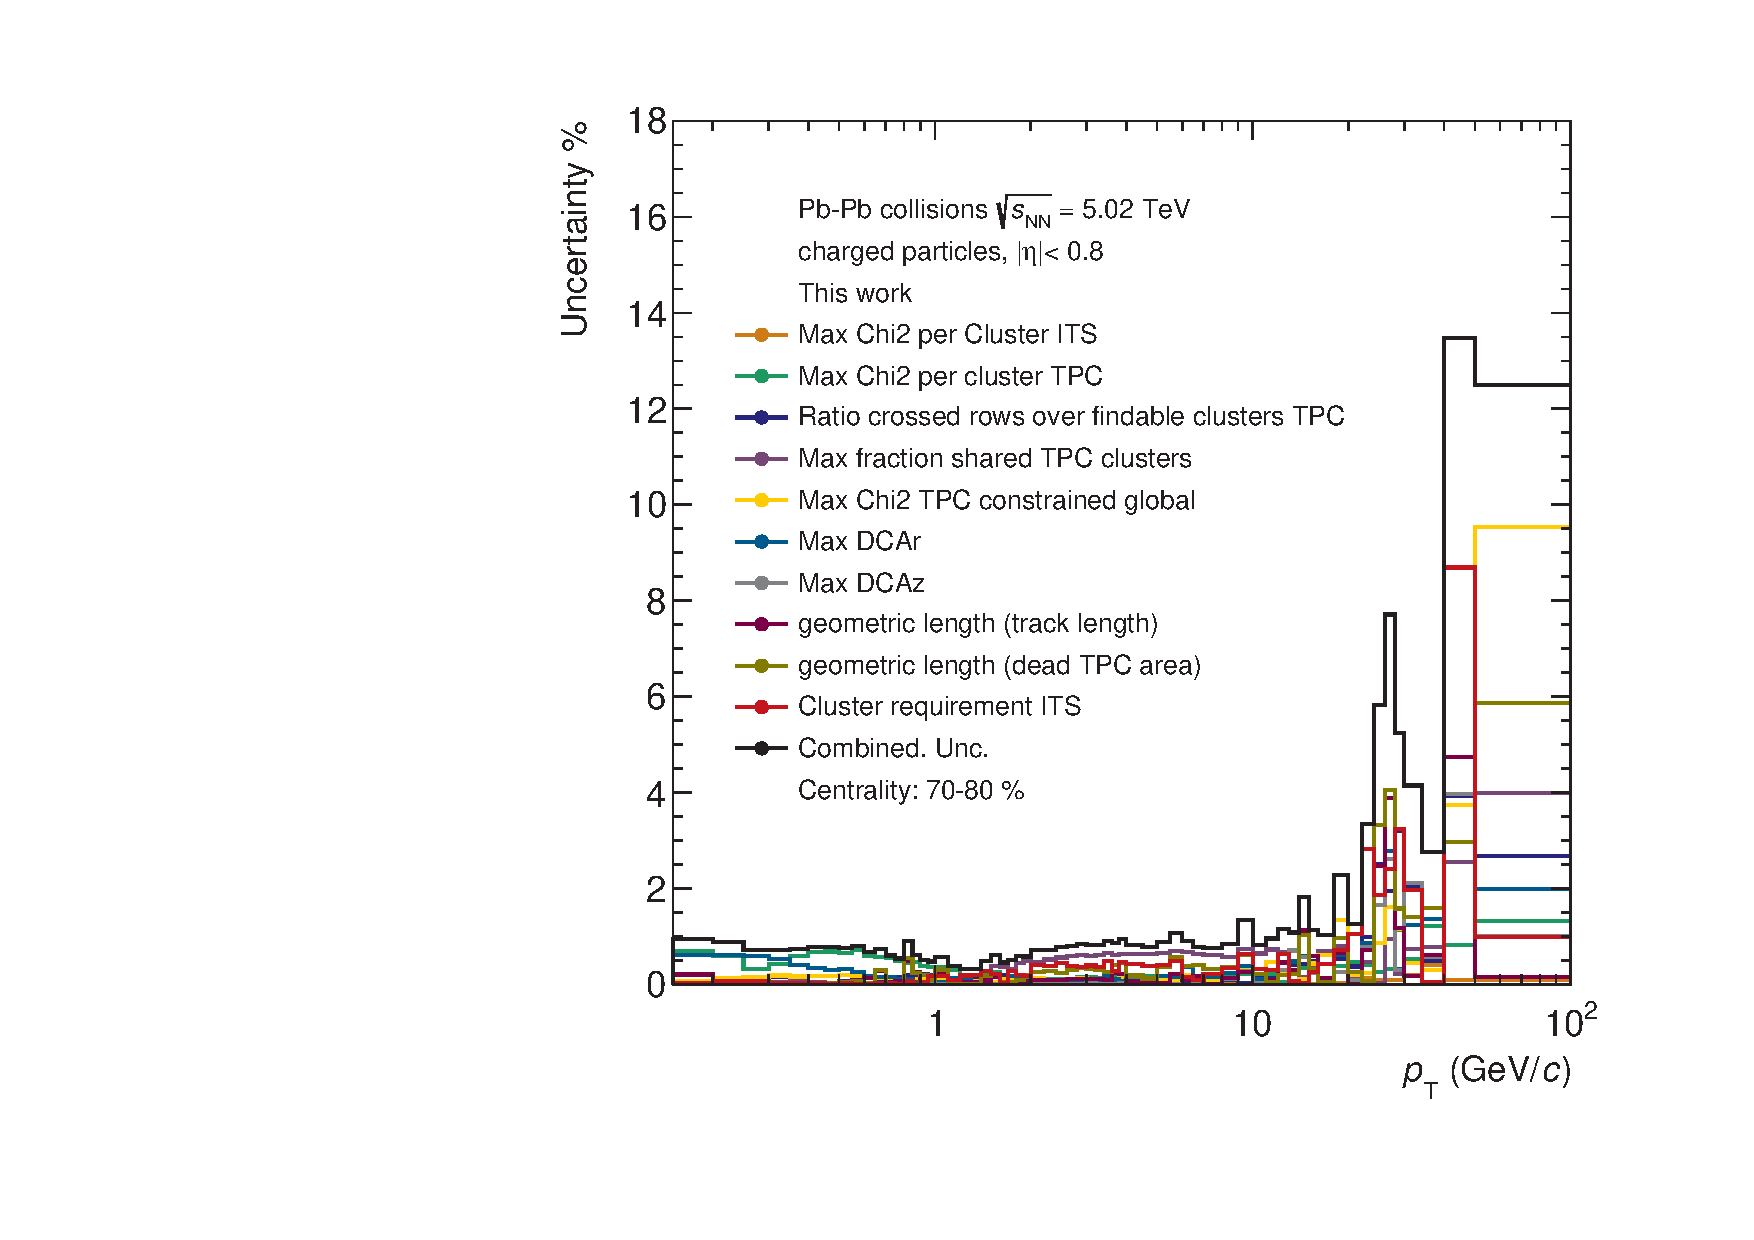
\includegraphics[width=0.495\textwidth]{Plots/SysUncRaaperi.pdf}  
\caption{Relative systematic uncertainties of $R_\text{PbPb}$ from the track selection for central, semi-central  and peripheral Pb-Pb collisions.}
\label{SysUncRaa}
\end{figure}
As explained in Section \ref{TrackSelection}, the track selection criteria have been developed and validated in the course of the last years. Nevertheless, the choice of the selection criteria, yet justified via cross-checks, is subjected to a systematic uncertainty. The total value of $\sigma^\text{sys}_\text{tot}$ is calculated via the root sum squared method over the individual contributions to the systematic uncertainties, which are assumed to contribute independently of the rest. For this reason, :
\begin{equation}
\sigma^\text{sys}_\text{sel,tot} = \sqrt{\sum_{\text{i}}\left(\sigma^\text{sys}_\text{sel,i} \right)^2}
\end{equation} 
To determine the individual contributions, each nominal track requirement listed in Table \ref{tab:Cuts} is varied twice within a range in which it is believed to be physically meaningful. The variations, listed in Table \ref{tab:curVar}, correspond to the maximum and the minimum of this range. Next, the fully corrected \pt distributions are recalculated with each variation. The ratio of these \pt spectra to the nominal one is determined, obtaining as result two ratios for each track cut, with the exception of the required hit in the SPD. The two ratios are evaluated in each \pt interval and the largest deviation from the nominal \pt spectrum between the both of them is assumed as systematic uncertainty in the corresponding \pt interval. The resulting systematic uncertainties corresponding to each track cut can then be presented as function of the transverse momentum. In Figure \ref{SysUncSpec}, the individual contributions and the combined systematic uncertainty are given for pp as well as for central, semi-central and peripheral Pb-Pb collisions. \\
In the previous ALICE measurement of nuclear modification factors, the corresponding systematic uncertainties were calculated by propagating the systematic uncertainties on the \pt distributions in pp and Pb-Pb collisions. With the aim of obtaining a more accurate estimation of the systematic uncertainties on $R_\text{Pb-Pb}$, the same approach explained above is used. In Figure \ref{SysUncRaa}, the resulting contributions are shown for pp as well as for central, semi-central and peripheral Pb-Pb collisions.
\begin{table}[H]
\renewcommand{\arraystretch}{1.5}
%\rowcolor{bodyBlue}
\centering
\begin{tabular}{l c c c}
\toprule
\rowcolor{headerBlue}  \textbf{Track parameter} &  \textbf{Condition}  &  \multicolumn{2}{c}{\textbf{Variations}} \\
\midrule
\multicolumn{4}{c}{\textbf{Selection of primaries}} \\
\midrule
$\text{DCA}_{z}$ & $\leq 2 $ cm & $1$ cm & $5$ cm\\
$\text{DCA}_{xy}$ & $\leq 7\sigma$ & $4\sigma$ & $10\sigma$ \\
\midrule
\multicolumn{4}{c}{\textbf{ITS selection}} \\
\midrule
at least one hit in the SPD & required  & \multicolumn{2}{c}{not required}\\
$\chi^2$ per ITS cluster  & $< 36$ & $\leq 25$ & $\leq 49$ \\
\midrule
\multicolumn{4}{c}{\textbf{TPC selection}} \\
\midrule
$\chi^2$ per TPC cluster (pp collisions) & $< 4.0$  & $\leq 3.0$ & $\leq 5.0$\\
$\chi^2$ per TPC cluster (Pb-Pb collisions) & $< 2.5$ & $\leq 1.7$ & $\leq 3.4$\\
fraction of shared  TPC clusters&  $<0.4$  & $\leq 0.2$ & $\leq 1.0$ \\
ratio of crossed rows over findable clusters  & $> 0.8$ & $\geq 0.7$ & $\geq 0.9$\\
geometric length (dead TPC area) & $3$ cm & $2$ cm & $4$ cm \\
geometric length (track length) & $130$ cm & $120$ cm & $140$ cm\\

\midrule
\multicolumn{4}{c}{\textbf{TPC-ITS selection}} \\
\midrule
$\chi^2$ TPC constrained track vs. global track  & $\leq 36$ & $\leq 25$ & $\leq 49$ \\
\bottomrule
\end{tabular}
\caption{Variations for the standard track selection criteria used for the calculation of the systematic uncertainties.}
\label{tab:curVar}
\end{table}
\subsection{Other sources of uncertainties} 
In previous measurements of inclusive charged particles (cite paper), other sources of systematic uncertainties on the \pt distributions besides the track selection have been identified. In this section, an overview about the corresponding sources as well as an approximation of their contributions to the total systematic uncertainties acquired from the cited publication will be given. In Table \ref{tab:othersources}, the relative systematic uncertainties for \pt spectra in pp and Pb-Pb collisions are shown. 
\begin{itemize}
\item The tracking efficiency is approximated using the MC information. Nevertheless, the simulations are not able  to reproduce fully the detector performance. The related systematic uncertainty is calculated by means of a quantity that compares ITS-TPC tracks with tracks reconstructed only with the TPC: the matching efficiency. The maximum deviation from unity of the ratio of the matching efficiency in MC to the one in data is used as uncertainty.
\begin{table}[tb!]
\renewcommand{\arraystretch}{1.5}
%\rowcolor{bodyBlue}
\centering
\begin{tabular}{l c c}
\toprule
\rowcolor{headerBlue}  \textbf{Source of uncertainty} &  \textbf{pp}  &   \textbf{Pb-Pb}  \\
\midrule
\midrule
Matching efficiency & $0.0$-$1.1\%$  & $0.2$-$1.2\%$\\
Particle composition & $0.2$-$2.4\%$ & $0.2$-$2.0\%$\\
Secondary scaling & $0.0$-$2.8\%$ & $0.0$-$4.5\%$ \\
Vertex and trigger efficiency & $0.0$-$1.2\%$ & - \\
Material budget & $0.1$-$0.9\%$ & $0.1$-$0.9\%$ \\
Anchor point & - & $0.06$-$3.5\%$ \\
\bottomrule
\end{tabular}
\caption{Contributions to the total systematic uncertainty on \pt distributions in pp and Pb-Pb collisions determined in the previous ALICE measurements (cite paper).}
\label{tab:othersources}
\end{table}
\item There are three distinct contributions to the systematic uncertainty of the particle composition correction related to assumptions during the development of the analysis (cite Patrick). For their calculation, variations in specific parameters of the procedure are performed and the maximal deviation between the nominal correction and the one resulting from each variation is assigned as systematic uncertainty. The total systematic uncertainty is determined by summing in quadrature the individual contributions:
\iffalse
\begin{itemize}
\item The first contribution is related to measured production rates of identified charged particles. The measured particle spectrum of each particle type are varied between the extreme values of the range of its systematic uncertainty.
\item Another contribution arises from the extrapolation of the \pt spectra at low \pt used in the correction. The contribution is estimated by recalculating the correction using alternative parametrizations as well as different fit ranges.
\item The last contribution originates from the fact that the relative particle abundances are assumed to be flat for $p_\text{T} > 10$ GeV/$c$. For the calculation of the systematic uncertainty, this range is varied and the resulting corrections are compared to the nominal one.  
\end{itemize} 
\fi
\item The contribution to the systematic uncertainties of the data-driven scaling of the secondary contamination is determined by comparing the correction factors that result from a two and a three template fit. The deviation between both results is assigned as uncertainty.
\item In the published results, the vertex and trigger efficiency is combined and the half of this value was assigned as systematic uncertainty.
\item The MC simulation of the detector response by the GEANT3 framework bears an uncertainty, which is determined by varying the material budget by $\pm 4.5\%$.
\item For the centrality determination in Pb-Pb collisions, an anchor point is defined as the reference limit of the centrality below which the measurement is biased (see Section \ref{centEstim}). Its determination is subject to an uncertainty of $0.5\%$. After adjusting the centrality boundaries with this uncertainty, \pt spectra are recalculated and the maximum deviation from the nominal one is assigned as the corresponding contribution.
\end{itemize} 
\section{Results}
\subsection{Differential cross section in pp collisions}
After implementing the corrections as described in Section \ref{secCorr}, the differential cross section (see Equation \ref{EqdiffCross}) for inclusive charged particles in inelastic pp collisions at $\sqrt{s}=5.02$ TeV measured by ALICE is presented in Figure \ref{diffCross}. The statistical uncertainties are shown in error bars, while the boxes represent the systematic uncertainties determined as described in Section \ref{systracksel}. In the figure, also the previous ALICE measurement (cite note) is also shown. It can be observed that the presented work reaches a transverse momentum of $p_\text{T} = 100$ GeV/$c$ which extends the \pt reach of the previous measurement of $p_\text{T} = 50$ GeV/$c$. This development is explained by the higher statistics that the used data sets offer in comparison to the ones of 2015. Another feature of this result is the improved granularity of the \pt intervals which are finer in the mid and high \pt region than in the previous measurements. These two aspects facilitate a better precision of the nuclear modification factors as it will be seen in the following sections. 
(da fehlt wahrscheinlich noch einen Absatz)
\begin{figure}[tb!]
\centering
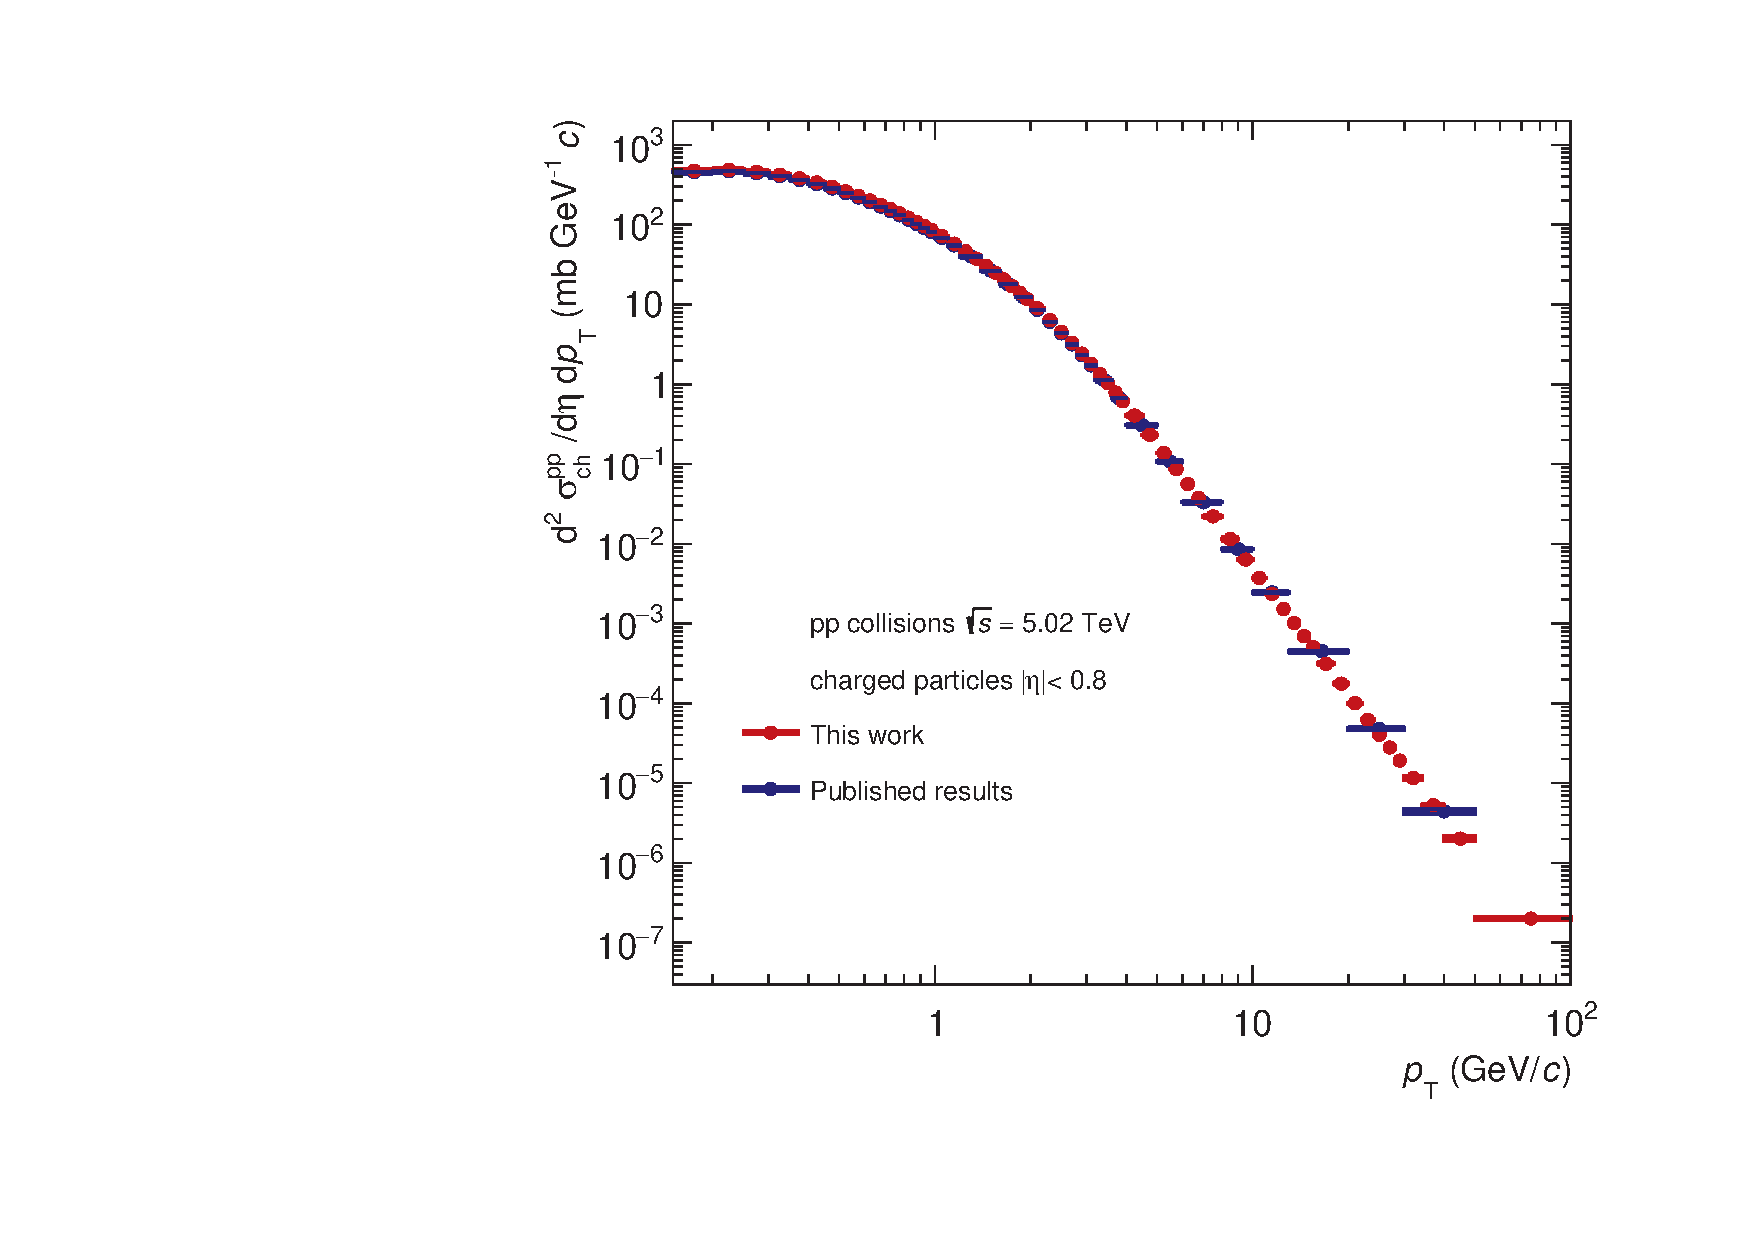
\includegraphics[width=12cm]{Plots/diffCrosspp.pdf}  
\caption{Differential cross section for inclusive charged-particle production in pp collisions at $\sqrt{s}=5.02$ TeV measured by ALICE.}
\label{diffCross}
\end{figure}
\subsection{Invariant yield in Pb-Pb collisions}
The invariant yields (see Equation \ref{Eqinyield}) for inclusive charged particles in nine centrality classes in inelastic Pb-Pb collisions measured by ALICE at $\sqrt{s}_\text{NN}=5.02$ TeV are given in Figure \ref{invYield}. Statistical and systematic uncertainties are represented with error bars and boxes, respectively. In the same figure, the results of the previous ALICE measurement are also shown. The shape of the \pt distributions show a centrality dependence. In central collisions, the invariant yields present a more pronounced slope for \pt > 3 GeV/$c$ than the one in peripheral collisions. With decreasing centrality the shape becomes more similar to the one in pp. Once the fully \pt distributions in pp and in Pb-Pb collisions are determined, the nuclear modification factors are calculated.
\begin{figure}[tb!]
\centering
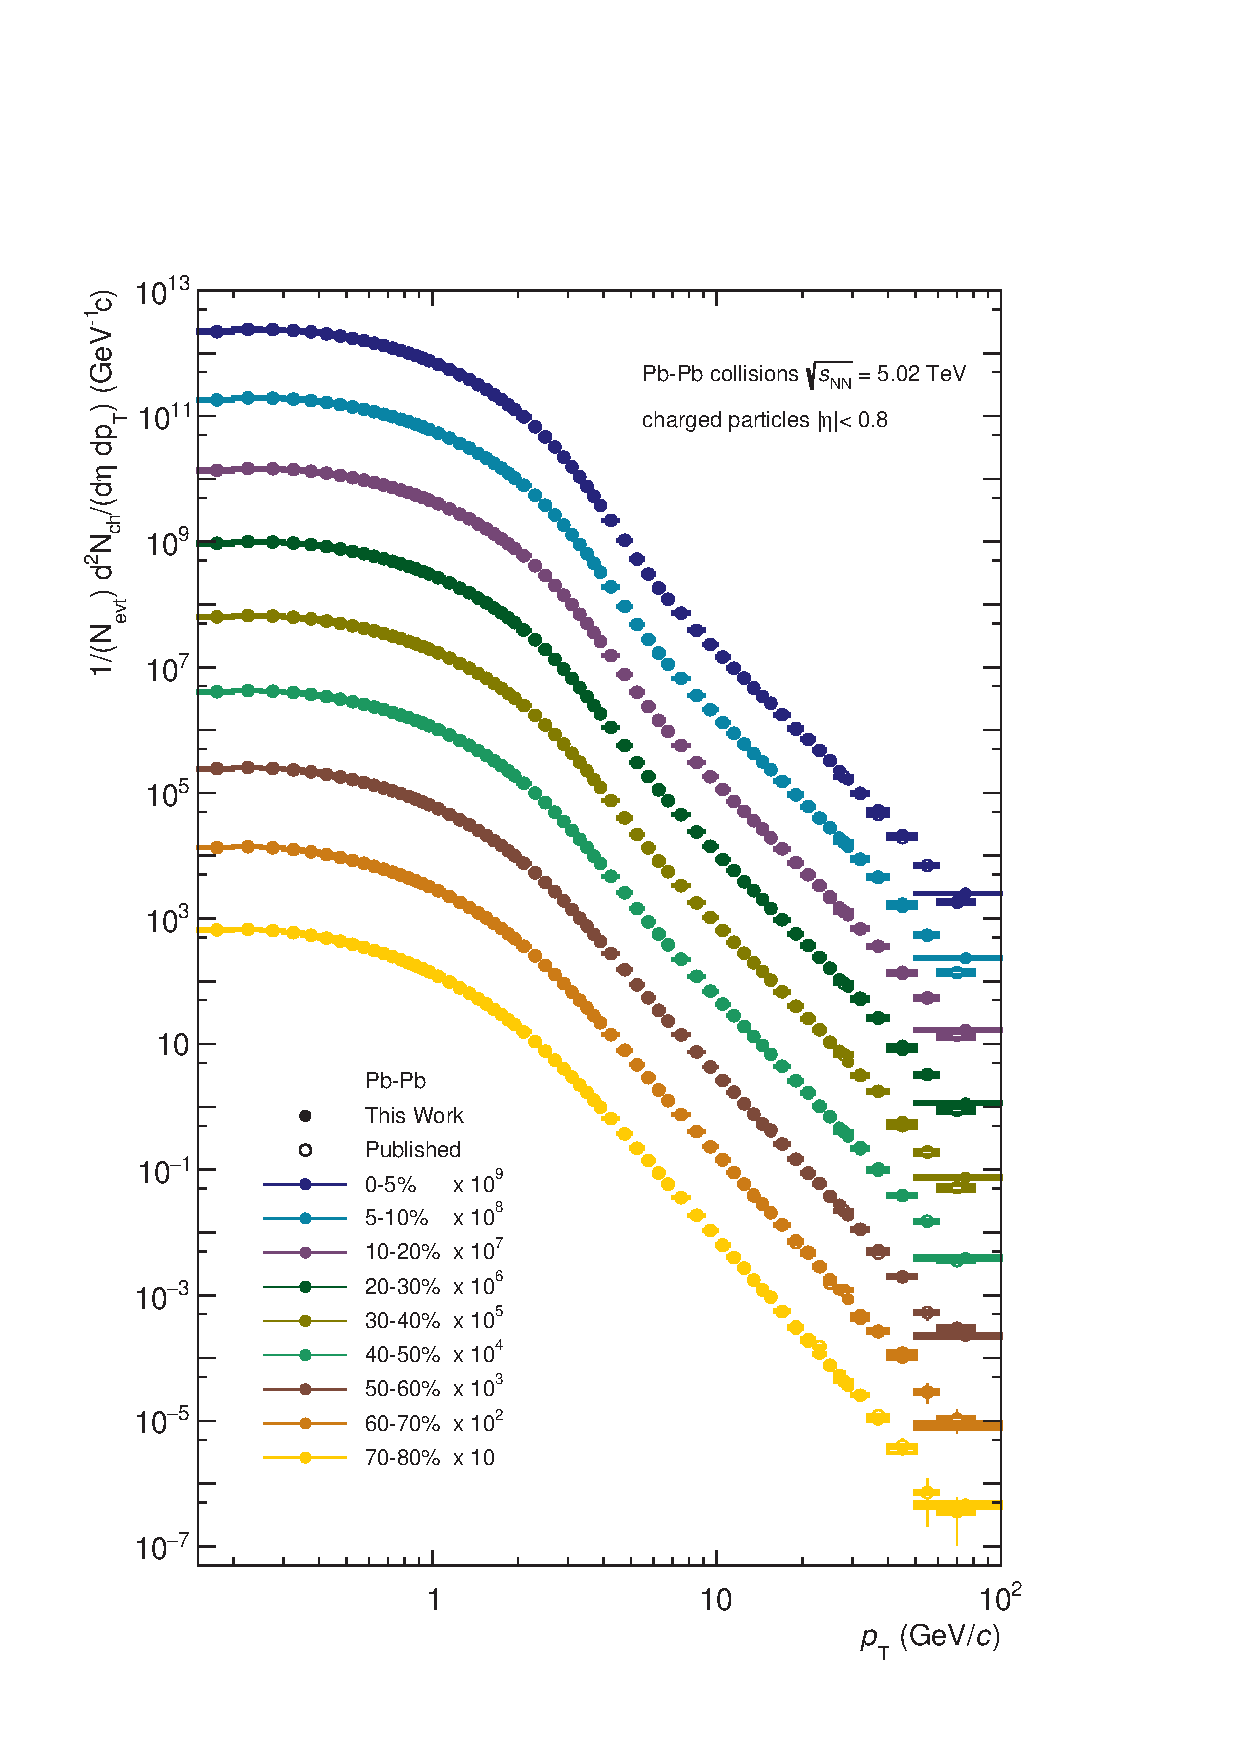
\includegraphics[width=12cm]{Plots/invYieldPbPb.pdf}  
\caption{Differential cross section for inclusive charged-particle production in pp collisions at $\sqrt{s}=5.02$ TeV measured by ALICE.}
\label{invYield}
\end{figure}
\subsection{Nuclear modification factors}
As introduced in Section (cite section), the energy density produced in ultra-relativistic heavy-ion collisions  allows the creation of a QGP, a deconfined state of strongly interacting matter. In this medium, high \pt partons experience an energy loss which leads to a suppression of the particle production as it was suggested by J.D. Bjorken (cite here). The study of this suppression can therefore provide insight on the properties of the QGP. In the presented work, the suppression is analyzed by comparing the charged-particle production in heavy-ion collisions with a reference measurement in pp collisions, where no QGP is expected to be created. The nuclear modification factor $R_\text{PbPb} $ offers the possibility to quantify the suppression via:
\begin{equation}
R_\text{PbPb} = \dfrac{1}{\langle T_\text{AA}\rangle} \dfrac{\text{d}^2 N^\text{Pb-Pb}_\text{ch} / \text{d}\eta \text{d}p_\text{T}}{\text{d}^2 \sigma^\text{pp}_\text{ch} / \text{d}\eta \text{d}p_\text{T}}
\end{equation}
where the numerator represents the invariant yield in Pb-Pb collisions and the denominator the differential cross section in pp collisions. Note that the differential cross section is scaled with the nuclear overlap function $\langle T_\text{PbPb} \rangle$. This quantity is calculated through a Glauber Monte Carlo simulation (cite ana note) and the values used in this work can be found in Table \ref{tab:taa}.\\
\begin{table}[tb!]
\renewcommand{\arraystretch}{1.5}
%\rowcolor{bodyBlue}
\centering
\begin{tabular}{l c c}
\toprule
\rowcolor{headerBlue}  \textbf{Centrality} &  \textbf{$\mathbf{\langle T_\text{PbPb} \rangle}$ ($\text{mb}^{-1}$)}  &   \textbf{sys. Unc. } ($\text{mb}^{-1}$) \\
\midrule
\midrule
0-5\% & $26.08$  & $0.176$\\
5-10\% & $20.44$ & $0.166$\\
10-20\% & $14.4$ & $0.126$ \\
20-30\% & $8.767$ & $0.101$ \\
30-40\% & $5.086$ & $0.0814$ \\
40-50\% & $2.747$ & $0.0486$\\
50-60\% & $1.352$ & $0.0309$\\
60-70\% & $0.5992$ & $0.0158$\\
70-80\% & $0.2385$ & $0.00552$ \\
\bottomrule
\end{tabular}
\caption{Nuclear overlap function with the corresponding systematic uncertainties for Pb-Pb collisions at $\sqrt{s}_\text{NN}=5.02$ TeV in the studied centrality classes obtained with a Glauber Monte Carlo simulation (cite ana note).}
\label{tab:taa}
\end{table}
In Figure \ref{Raa}, the nuclear modification factors for inclusive charged particles in inelastic Pb-Pb collisions measured by ALICE at $\sqrt{s}_\text{NN}=5.02$ TeV are presented in nine centrality classes. The statistical uncertainties are denoted as error bars and the systematic uncertainties as boxes. As expected, the nuclear modification factors are characterized by a strong dependency on the centrality. In the same figure, the previous measurements of nuclear modification factors in ALICE are also shown with open markers. The results of this work are in good agreement with the ones of the previous measurement. There is an improvement of the \pt reach as well as of the granularity of the intervals for \pt > 3.2 GeV/$c$. This is a result of the increased statistics in pp collisions which allows a better precision in the corresponding \pt distribution as described before.\\
A significant suppression of the charged-particle production is observed in most \pt intervals of the nine centrality classes. In the low \pt region, the suppression decreases slightly until the $R_\text{PbPb}$ reach values of around 0.45 in the most central collisions and around 0.8 in peripheral collisions. Following this peak, the maximal suppression occurs at around \pt = 6.5 GeV/$c$ for the first four centrality classes, before the nuclear modification factors rise gradually and reach values between around 0.5 and 0.6. Towards peripheral collisions, the fall after the peak is less pronounced, the factors grow more steeply and the values of $R_\text{PbPb}$ approach unity at high transverse momenta. 
\begin{figure}[tb!]
\centering
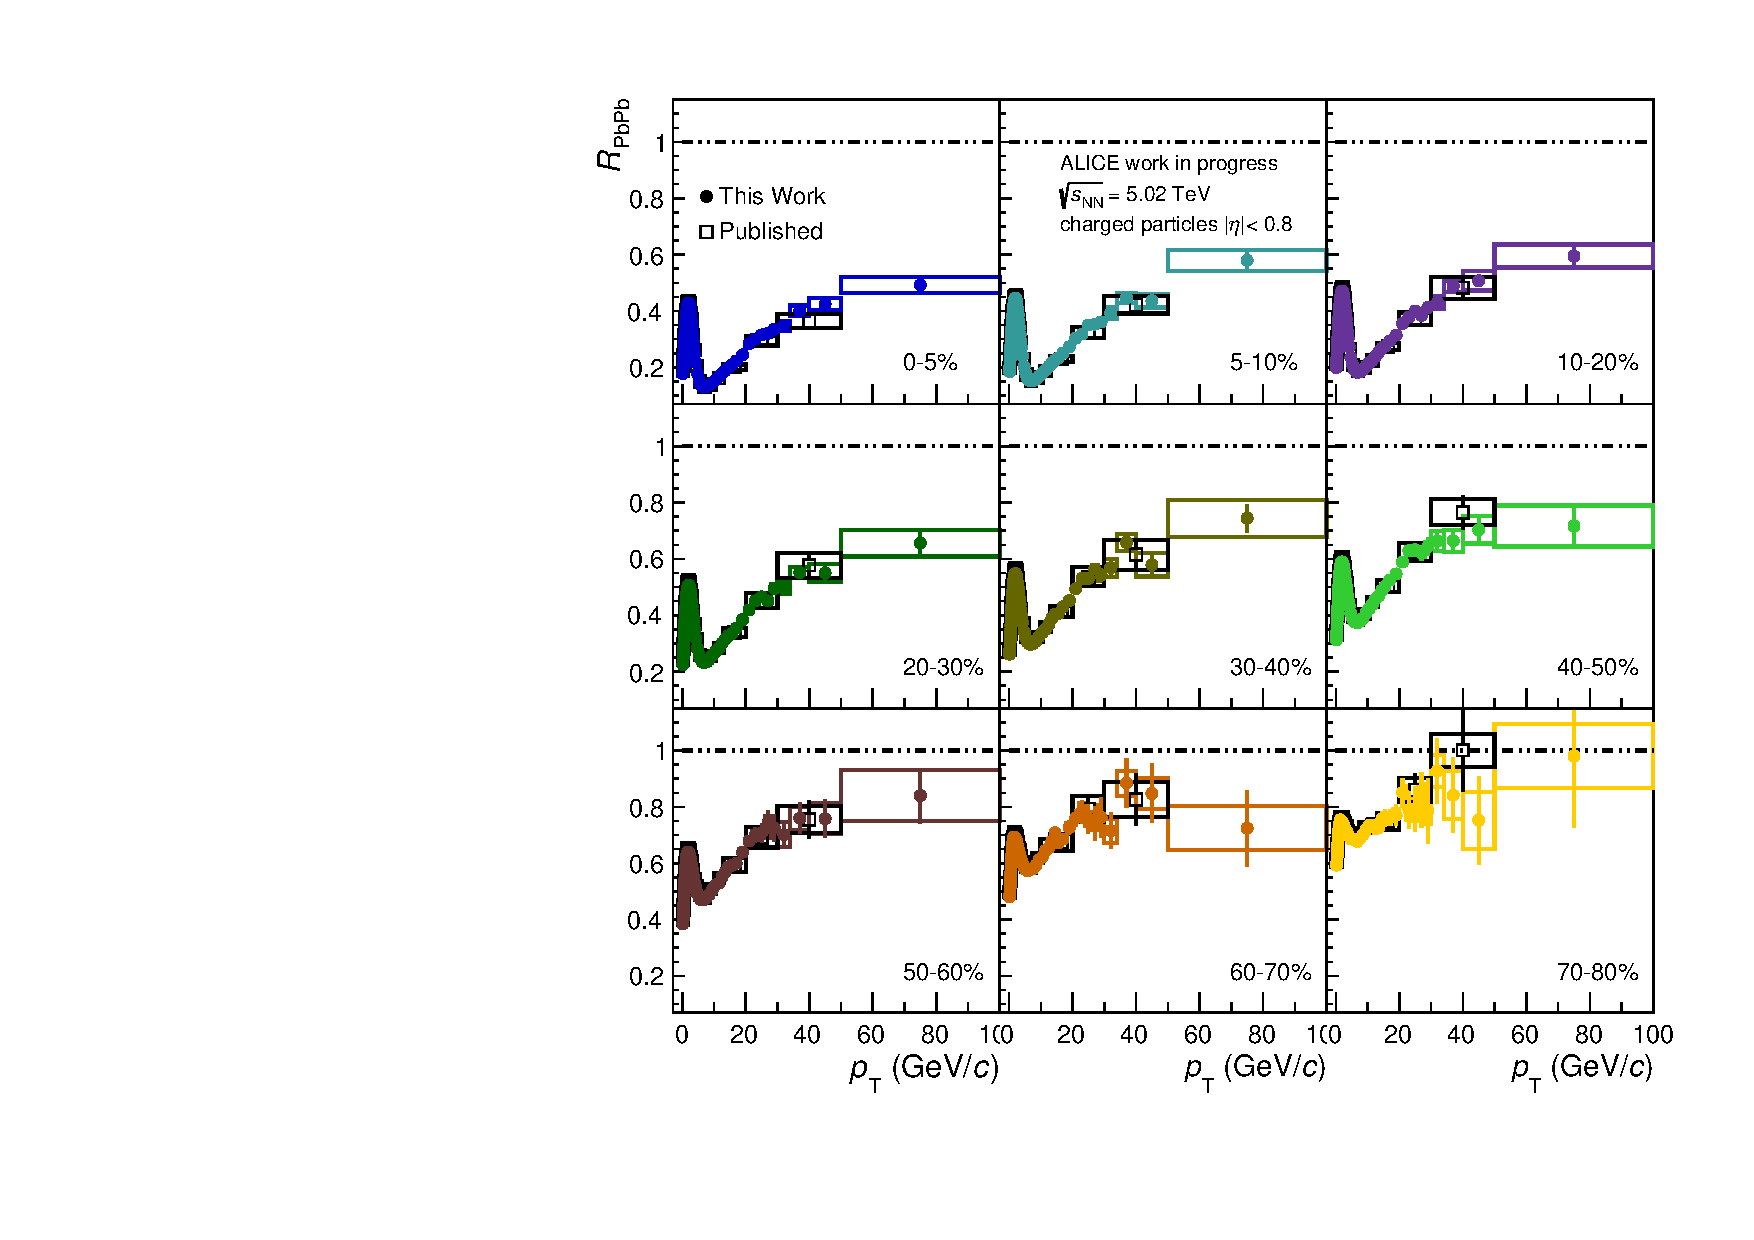
\includegraphics[width=15.5cm]{Plots/Raa.pdf}  
\caption{Nuclear modification factors for nine centrality classes in Pb-Pb collisions at $\sqrt{s}=5.02$ TeV measured by ALICE.}
\label{Raa}
\end{figure}
For a better understanding of the suppression in heavy-ion collisions, several theoretical models make predictions about the influence of the strong interacting medium produced at LHC energies on the charged-particle production. For the validation of the measured nuclear modification factors, is worth comparing them with the theoretical models. The model calculations make use of a pQCD factorization of the cross section for hadron production. All of the following models implement different approaches which lead to parton energy loss. Therefore, a comparison of these measurements with the models will help to improve the fundamental understanding of parton energy loss mechanisms. The formalisms of each of the approaches are presented briefly in the following (cite paper):
\begin{figure}[tb!]
\centering
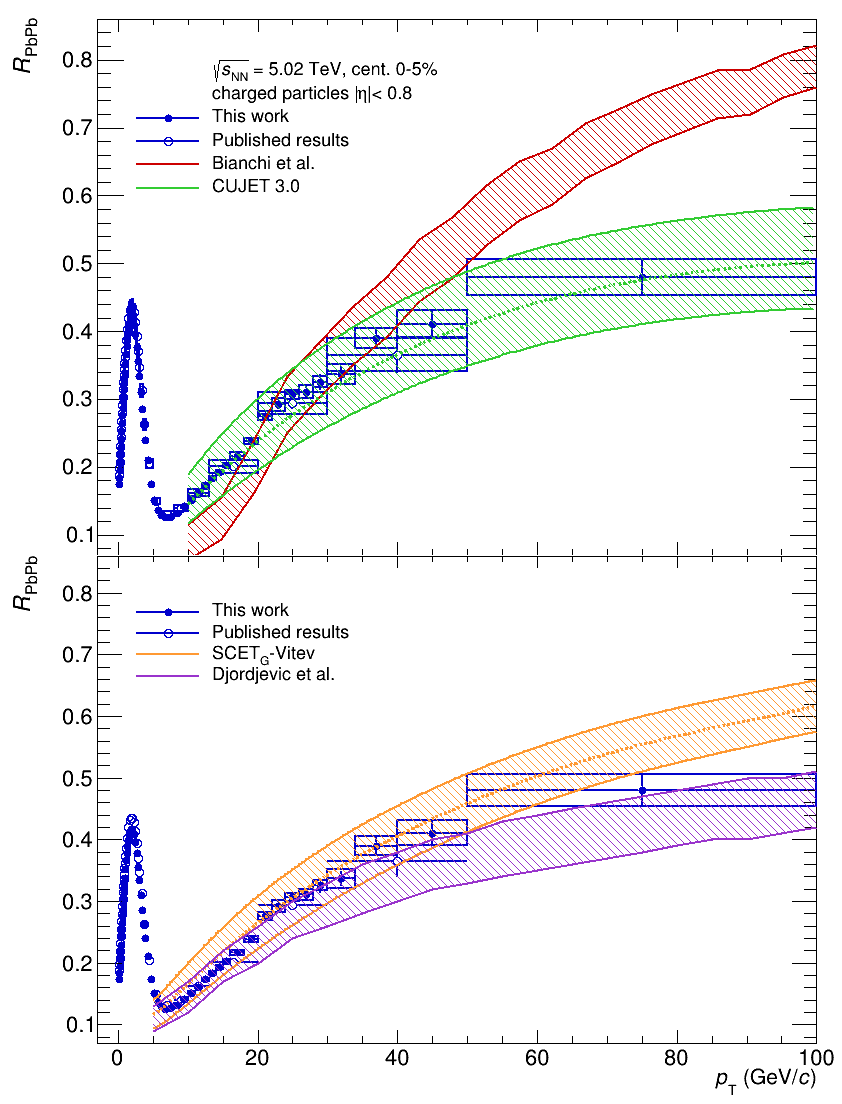
\includegraphics[width=10cm]{Plots/Raatheo.png}  
\caption{Nuclear modification factors for the most central collisions in Pb-Pb collisions at $\sqrt{s}=5.02$ TeV compared to four theoretical prediction as well as to the previous ALICE publication.}
\label{raatheo}
\end{figure}

\begin{itemize}
\item \textbf{Bianchi's model (cite here):} this model describes the production of high \pt hadrons with the fragmentation of hard partons. In a framework based on the hydrodynamics, the energy loss of the parton is characterized by the medium transport coefficient $\hat q$ scaled with the temperature dependent entropy density and the energy scale of jets within the medium.
\item \textbf{CUJET 3.0:} the pQCD formalism provided by its predecessor CUJET 2.0 is upgraded with a description of soft processes by means of a suppression of quark and gluon degrees of freedom and the emergence of chromomagnetic monopoles. The model prediction is calculated by varying the QCD running coupling and the ratio of electric to magnetic screening scales. 
\item $\mathbf{SCET}_\mathbf{G}$-\textbf{Vitev's model (cite here):} this description of inclusive particle production and the suppression consists in the soft-collinear effective theory (SCET) extended with the coupling of Glauber gluons exchanges to the medium. In the calculations, cold nuclear matter effects and parton-to-hadron fragmentation functions are taken into account.
\item \textbf{Djordjevic's model (cite here):} the energy loss is predicted with pQCD calculations in a dynamical QCD medium of finite spatial extent. In the framework of the $\text{SCET}_\text{G}$ model, the prediction discusses the radiative and the collisional energy loss of the partons integrating cold nuclear effects.
\end{itemize}
In Figure \ref{raatheo}, the measured nuclear modification factor for a centrality of 0-5\% is compared to the four theoretical models as well as to the previous ALICE measurement. The upper and lower boundaries of the models represent the uncertainty which is calculated through variation of different parameters of the corresponding approaches. The measured nuclear modification factors are overall consistent with CUJET 3.0 and the models of Vitev and Djordjevic. It is worth pointing out, the similar agreement of the Vitev and Djordjevic calculations with the results although only the later includes predictions of the collisional energy loss. On the other hand, the Bianchi model overestimates the suppression in the \pt range 10 < \pt < 18 GeV/$c$, a trend already observed in the previous measurements. Nevertheless, the improvements in the nuclear modification factors allow to make better distinction at very high $p_\text{T}$. By that, it can be now stated that this model clearly deviates from the measured results since for \pt > 50 GeV/$c$ it also underestimates the data. As proposed at the beginning of this work, the increase of the data sample statistics leads hence to a better understanding of the nuclear modification factors.

\chapter{Summary}

\begin{appendices}
\chapter{Appendix}
\section{Tracking efficiency}
\label{TrkEffApp}
\end{appendices}

%, by virtue of its technical characteristics
%underlying
%drawbacks
%coined
%establishes
%is resolved
%streamlined
%resemble
%yields
%pronounced
%stand-alone
%exploting
%exhibit
%these outliers
%exemplify
%arises (from the fact)
%build upon
%notions
%conceive
%gathered data
%data collections
%procedure
%overall
%accounts for
% The way in which this is done
%  It is worth pointingout


%Quellen: https://home.cern/science/physics/standard-model
%An Introduction to Particle Physics and the Standard Model by Robert Mann
%An Introduction to Particle Physics and the Standard Model of Particle Physics by Cottingham and Greenwood
%Physics Of The Standard Model And Beyond, The Chong-sa Lim, Toshiyuki Morii,
%Data sample: https://twiki.cern.ch/twiki/bin/view/ALICE/AliDPGReconstructedDataTakingPeriodsSummarypp5

\end{document}
